\chapter{Results and Discussion: Zonal Based Adaptation/Refinement}

In chapter \ref{adapt_strat}, we established that the zonal based refinement/adaptation is the best strategy for computing accurate numerical solution using VMS-based error estimator driven mesh adaptation. In this chapter, we focus on applying the zonal based adaptation/refinement strategy to the low Reynolds number case of $Re=40,000$ at angle of attack $\alpha=6^\circ$ and advance ratio of $\mu_{sect}=1.2$ till we obtain mesh convergence. Here, we also perform an in-depth study of how spanwise resolution of the mesh affects the solution.

The nomenclature used for the different meshes, and mesh details are as follows:

[insert table with mesh names and mesh details here]


\section{Force Response}

A comparison of force response in the form of normalized lift and drag forces is shown in Figures \ref{fig:lift_zonal_adapt} and \ref{fig:drag_zonal_adapt} respectively. The normalized lift compares well for all the meshes considered. Normalized drag shows differences for Mza2 meshes and Mza3 meshes from M0 and Mza1 meshes. Maximum drag in the advancing phases is observed around $\psi=270^\circ$, with Mza3 meshes predicting slightly higher drag than Mza2 meshes, followed by Mza1 and M0 meshes. Major differences in drag between different meshes are observed specifically between phases $\psi=160^\circ$ and $\psi=240^\circ$. Between these phases, Mza2 and Mza3 meshes compare well with each other, whereas M0 and Mza1 meshes predict lower drag than Mza2 and Mza3 meshes. Note that lift and drag response remains unaffected with changes in spanwise resolution for the same in-plane mesh.

\begin{figure}[H]
\centering

\begin{subfigure}[b]{0.7\textwidth}
\centering
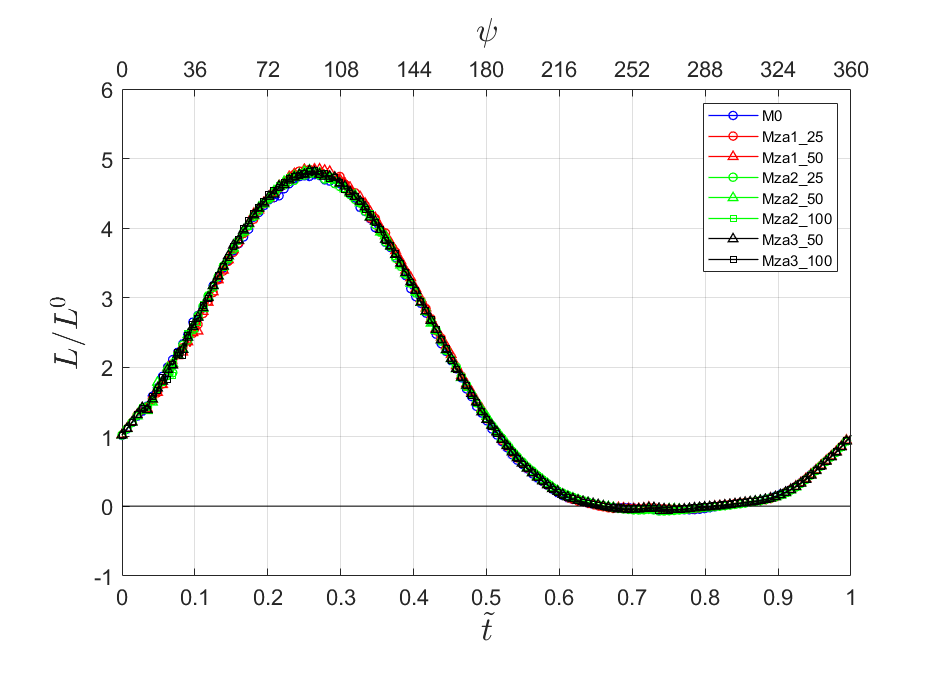
\includegraphics[width=1\textwidth]{figures/zonal_adapt_results/force_response/Lift.png}
\caption{Normalized lift}
\label{fig:lift_zonal_adapt}
\end{subfigure}
\begin{subfigure}[b]{0.7\textwidth}
\centering
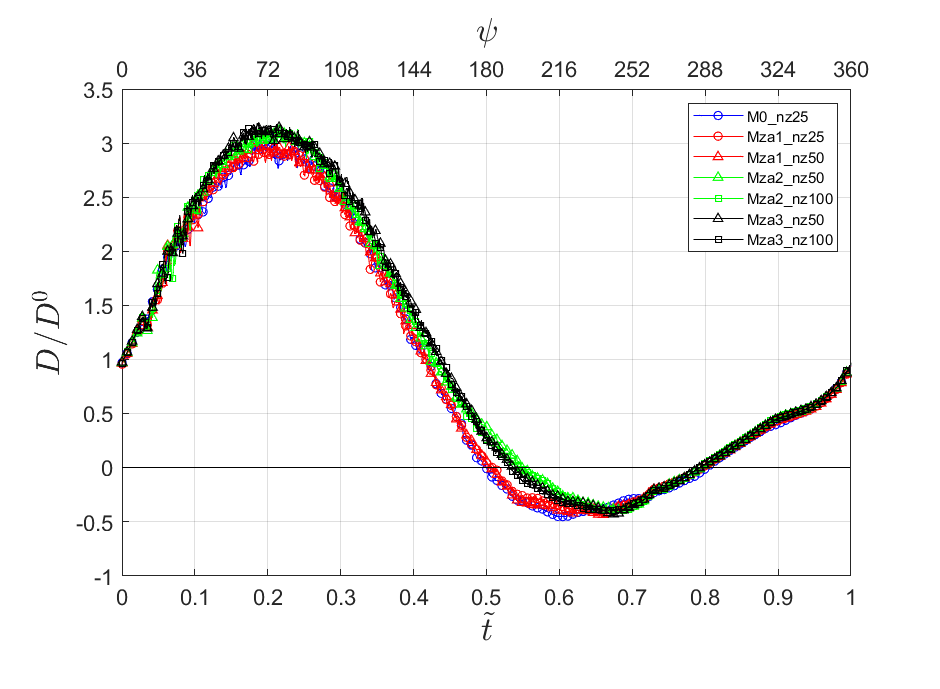
\includegraphics[width=1\textwidth]{figures/zonal_adapt_results/force_response/Drag.png}
\caption{Normalized drag}
\label{fig:drag_zonal_adapt}
\end{subfigure}

\label{fig:force_response_zonal_adapt}
\caption{Normalized forces for different meshes}
\end{figure}
\label{sec:zonal_force_response}

\section{Flowfield: Spanwise Vorticity}
<<<<<<< HEAD



In this section, we focus on instantaneous spanwise vorticity for the different meshes considered due to zonal-based refinement/adaptation. Here, instantaneous data is considered since we are interested in observing the flow structures and turbulence captured by different meshes, and obtaining phase-averaged data over multiple cycles can be computationally expensive, especially for the finer meshes, and can also filter out the turbulence in the flow-field.

A comparison of instantaneous spanwise vorticity for the different meshes is shown in Figures \ref{fig:vorticity_zonal_150}, \ref{fig:vorticity_zonal_180}, \ref{fig:vorticity_zonal_210}, \ref{fig:vorticity_zonal_240}, and \ref{fig:vorticity_zonal_270} for phases $\psi=150^\circ$, $\psi=180^\circ$, $\psi=210^\circ$, $\psi=240^\circ$, and $\psi=270^\circ$ respectively. 

For $\psi=150^\circ$, as the airfoil decelerates, the boundary layer over the airfoil starts to roll-up towards the geometric leading edge. The finer meshes, Mza2 and Mza3 show a thicker boundary layer along with more resolution of turbulence/fine-scale structures, than
the coarser meshes, M0 and Mza1.

For $\psi=180^\circ$, Mza2 and Mza3 meshes show a thicker boundary layer roll-up towards the geometric leading edge over the airfoil surface, as compared to $\psi=150^\circ$, along with significant flow separation. M0 and Mza1 meshes fail to capture a significant boundary layer roll-up at this phase. Moreover, Mza2 and Mza3 meshes capture more turbulence than M0 and Mza1 meshes, with the flow-structures captured by Mza2 meshes being slightly more diffused than Mza3 meshes. Note that changes in spanwise resolution for the same in-plane mesh do not show any significant variations in the flow-field.

For $\psi=210^\circ$, formation of LEV begins to take place for all meshes apart from M0, as we see a distinct vortex build up near the geometric leading edge, which M0 mesh fails to capture. There is a clear difference between both the location of the roll-up over the airfoil surface, and the size and extent of the roll-up between Mza1 meshes and Mza2 and Mza3 meshes. The flow-field for Mza2 and Mza3 meshes compare well with each other, with some minor differences due to the flow-field being instantaneous. More fine-scale flow structures are resolved by the finer meshes Mza2 and Mza3, while M0 and Mza1 show poor resolution of these structures.

At $\psi=240^\circ$, the LEV has ejected from the airfoil surface into a distinct vortex. Once again, a clear difference can be observed between the coarser meshes (M0 and Mza1 meshes) and the finer meshes Mza2 and Mza3, both in position, size, and extent of the LEV core, and also the turbulence captured around the LEV core. The coarsest mesh, M0, shows poor resolution of the shear layer, LEV, and the fine scale structures around it. Mza1\_25 and Mza1\_50 meshes show a similar location, size, and extent of the LEV, while resolving some diffused flow structures around it. Mza2 and Mza3 meshes compare well with each other in terms of the shear layer, LEV location, size, and extent, as well as the fine scale structures resolved. Once again, note that changes in spanwise resolution for the same in-plane mesh do not show any significant variations in the flow-field. 

At $\psi=270^\circ$, M0 mesh shows poor resolution with a diffused LEV core as compared to the other meshes, along with poor resolution of the shear layer. Mza1 meshes show a less diffused LEV core as compared to M0 mesh, however, the shear layer has comparatively poor resolution when compared to the finer meshes Mza2 and Mza3. Mza1 meshes also show minimal fine scale structures around the LEV core, as compared to Mza2 and Mza3 meshes. The LEV and the shear layer are best resolved in Mza3 meshes, with Mza3 showing more fine scale structures around the LEV core than Mza2 meshes.

A more quantitive comparison of the LEV including tangential velocity profiles and LEV location for different phases in the surging cycle is mentioned in the following sections.

%%=====================================
%% Phase = 150
%%=====================================


\begin{figure}[H]
	\centering
	\begin{center}
		\begin{subfigure}[b]{0.475\textwidth}
			\centering
			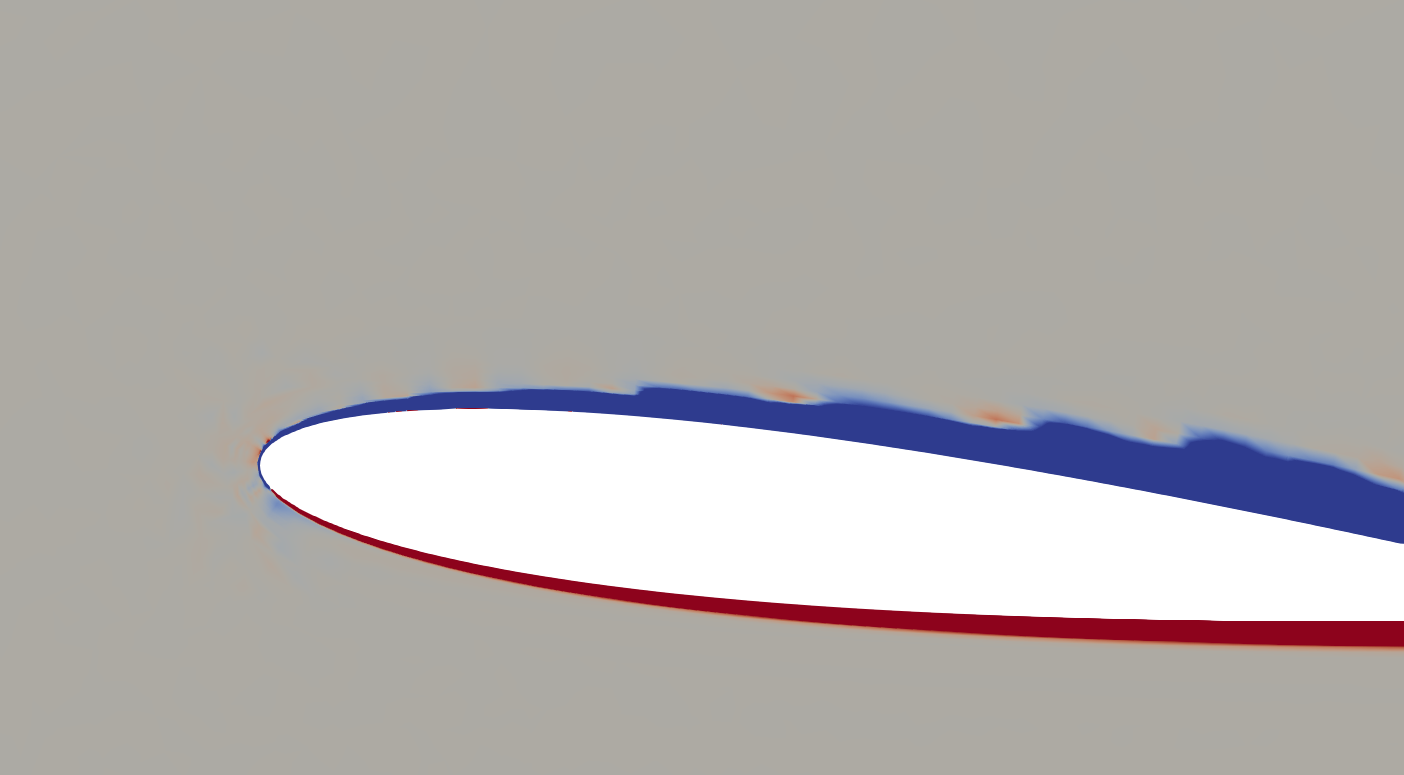
\includegraphics[width=1\textwidth]{figures/zonal_adapt_results/vorticity_plots/v2/M0/spavg/phase_150.png}
			\caption{M0 mesh, $\psi$ = $150^\circ$}
			\label{fig:M0_sp_psi150}
		\end{subfigure}
	\end{center}
	\begin{subfigure}[b]{0.475\textwidth}
		\centering
		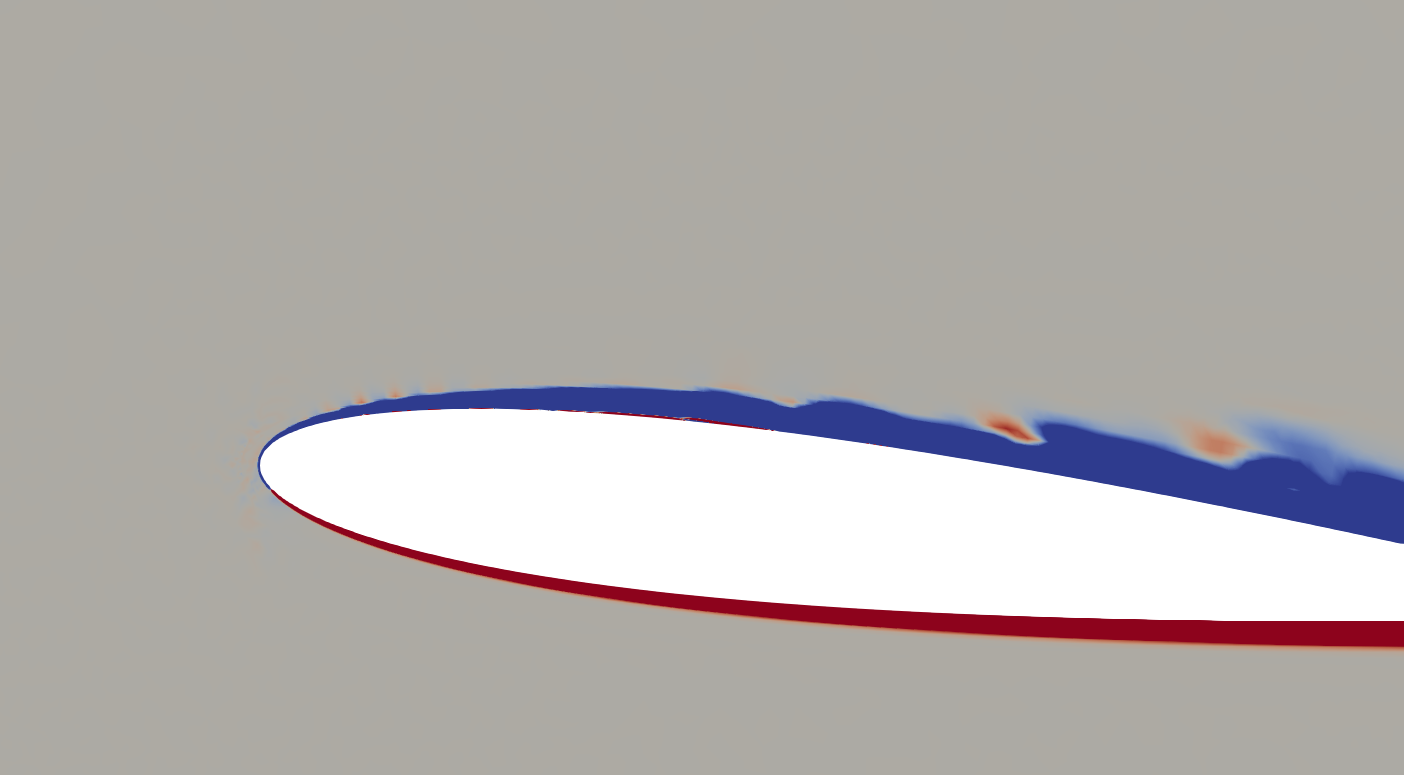
\includegraphics[width=1\textwidth]{figures/zonal_adapt_results/vorticity_plots/v2/Mza1_25/spavg/phase_150.png}
		\caption{Mza1\_25 mesh, $\psi$ = $150^\circ$}
		\label{fig:Mza1_25_sp_psi150}
	\end{subfigure}
	\begin{subfigure}[b]{0.475\textwidth}
		\centering
		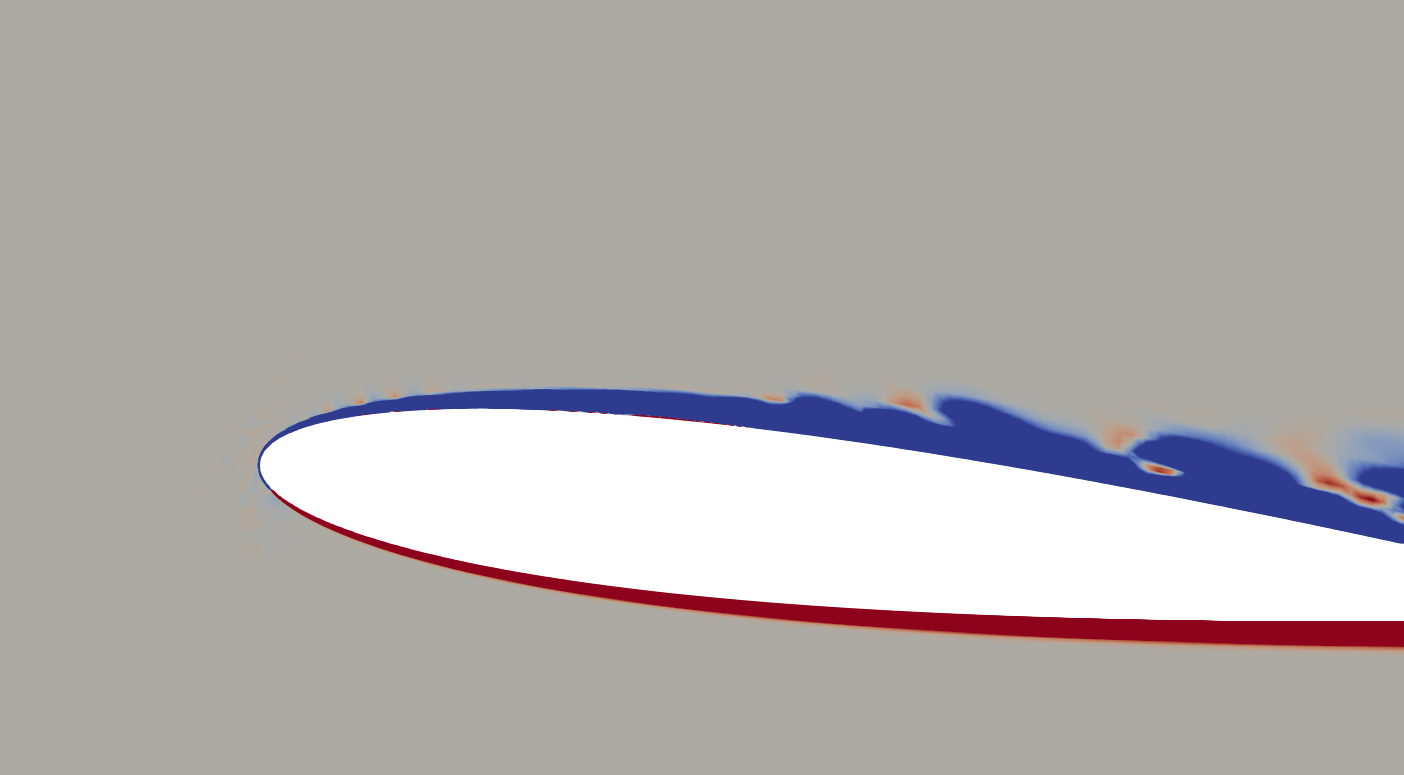
\includegraphics[width=1\textwidth]{figures/zonal_adapt_results/vorticity_plots/v2/Mza1_50/spavg/phase_150.png}
		\caption{Mza1\_50 mesh, $\psi$ = $150^\circ$}
		\label{fig:Mza1_50_sp_psi150}
	\end{subfigure}
	%	\begin{subfigure}[b]{0.475\textwidth}
	%		\centering
	%		\includegraphics[width=1\textwidth]{figures/zonal_adapt_results/vorticity_plots/v2/Mza1_100/spavg/phase_150.png}
	%		\caption{Mza1\_100 mesh, $\psi$ = $150^\circ$}
	%		\label{fig:Mza1_100_sp_psi150}
	%	\end{subfigure}
	%	\begin{subfigure}[b]{0.475\textwidth}
	%	\centering
	%	\includegraphics[width=1\textwidth]{figures/zonal_adapt_results/vorticity_plots/v2/Mza2_25/spavg/phase_150.png}
	%	\caption{Mza2\_25 mesh, $\psi$ = $150^\circ$}
	%	\label{fig:Mza2_25_sp_psi150}
	%	\end{subfigure}
	\begin{subfigure}[b]{0.475\textwidth}
		\centering
		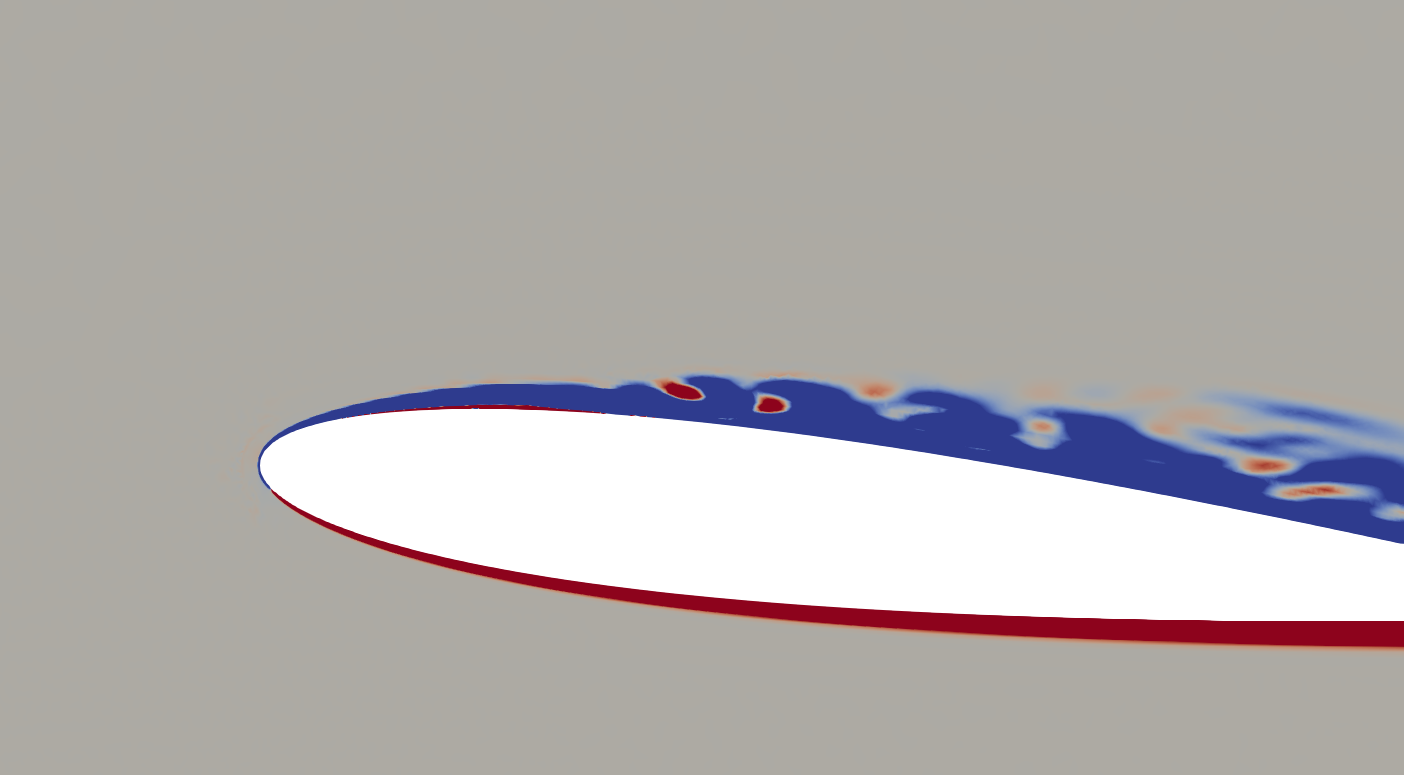
\includegraphics[width=1\textwidth]{figures/zonal_adapt_results/vorticity_plots/v2/Mza2_50/spavg/phase_150.png}
		\caption{Mza2\_50 mesh, $\psi$ = $150^\circ$}
		\label{fig:Mza2_50_sp_psi150}
	\end{subfigure}	
	\begin{subfigure}[b]{0.475\textwidth}
		\centering
		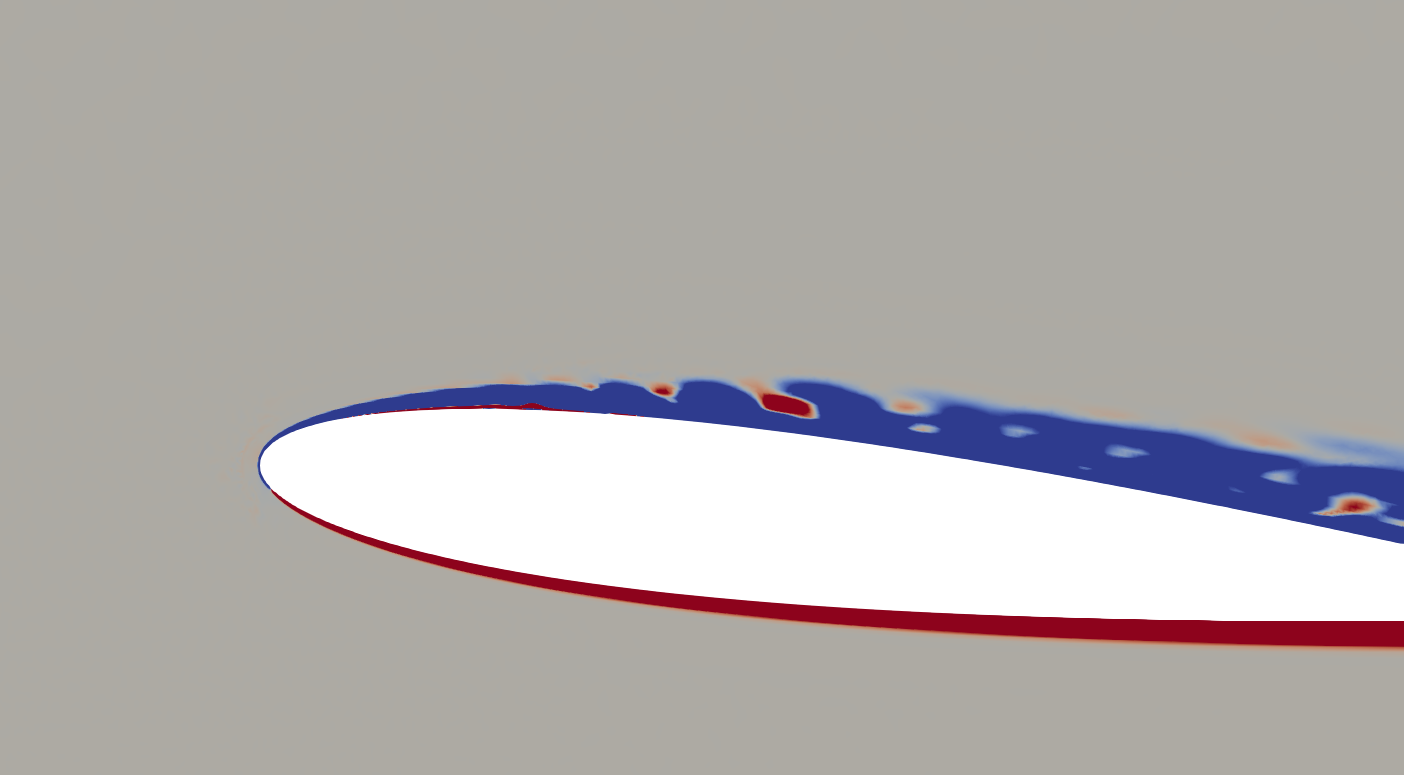
\includegraphics[width=1\textwidth]{figures/zonal_adapt_results/vorticity_plots/v2/Mza2_100/spavg/phase_150.png}
		\caption{Mza2\_100 mesh, $\psi$ = $150^\circ$}
		\label{fig:Mza2_100_sp_psi150}
	\end{subfigure}
	\begin{subfigure}[b]{0.475\textwidth}
		\centering
		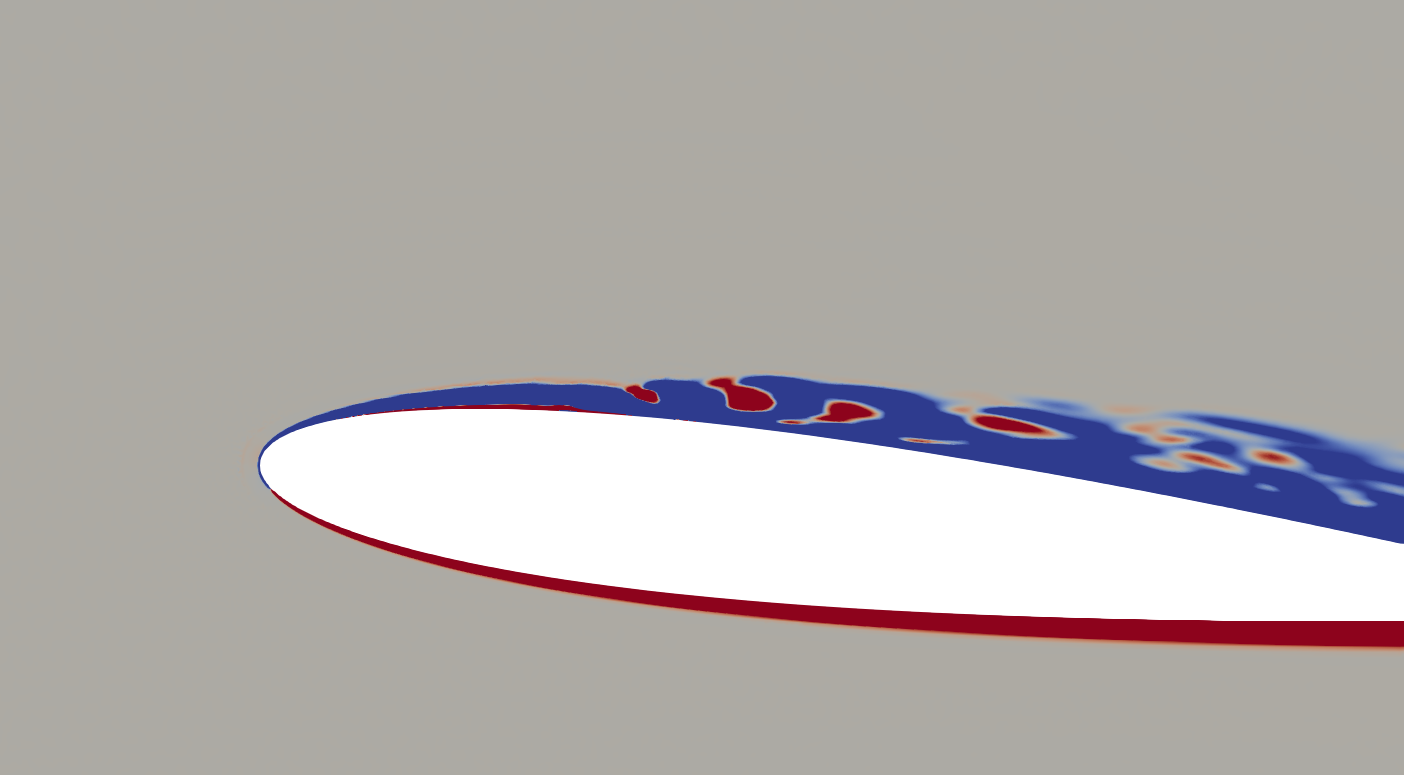
\includegraphics[width=1\textwidth]{figures/zonal_adapt_results/vorticity_plots/v2/Mza3_50/spavg/phase_150.png}
		\caption{Mza3\_50 mesh, $\psi$ = $150^\circ$}
		\label{fig:Mza3_100_sp_psi150}
	\end{subfigure}
	\begin{subfigure}[b]{0.475\textwidth}
		\centering
		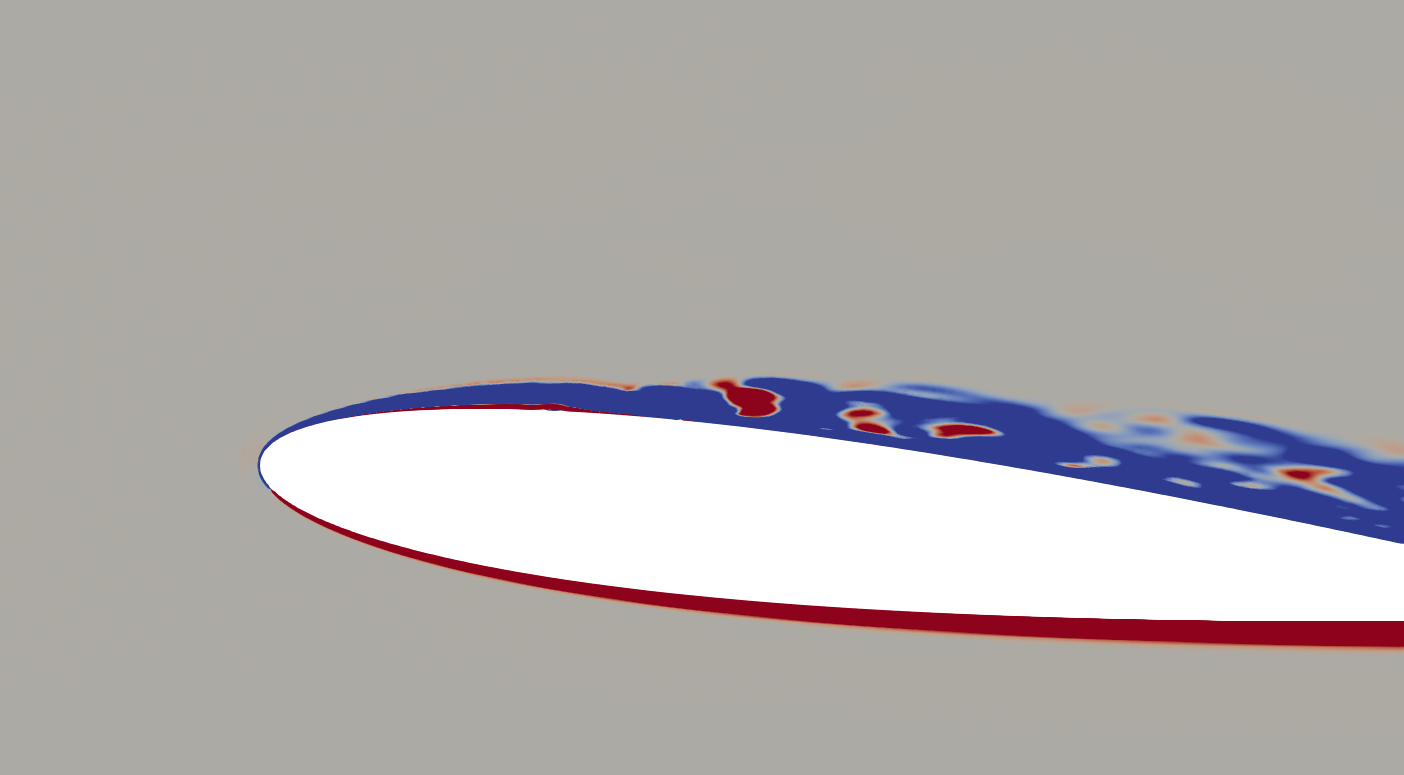
\includegraphics[width=1\textwidth]{figures/zonal_adapt_results/vorticity_plots/v2/Mza3_100/spavg/phase_150.png}
		\caption{Mza3\_100 mesh, $\psi$ = $150^\circ$}
		\label{fig:Mza3_100_sp_psi150}
	\end{subfigure}
	\caption{Spanwise vorticity comparison at $\psi$ = $150^\circ$ for different meshes}
	\label{fig:vorticity_zonal_150}
\end{figure}




%%=====================================
%% Phase = 180
%%=====================================


\begin{figure}[H]
	\centering
	\begin{center}
	\begin{subfigure}[b]{0.475\textwidth}
		\centering
		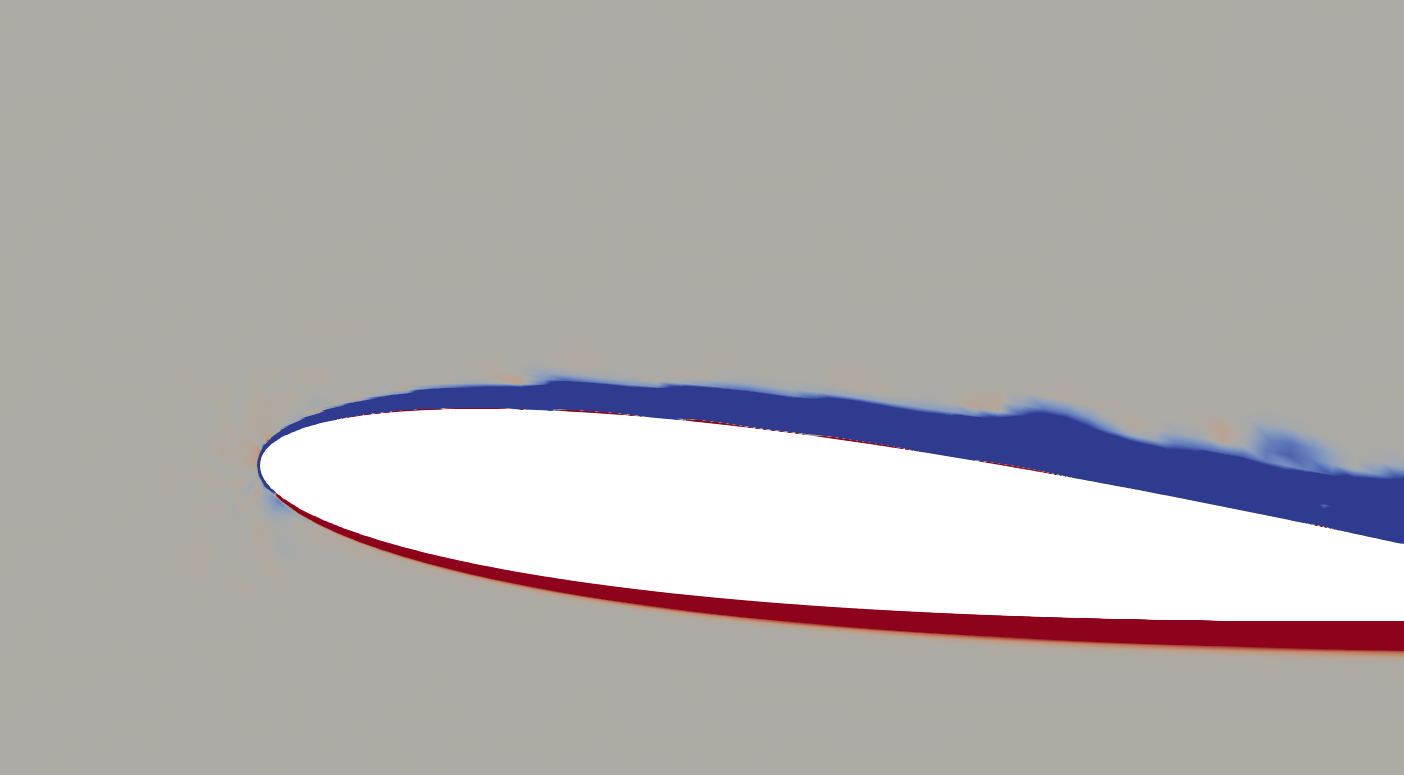
\includegraphics[width=1\textwidth]{figures/zonal_adapt_results/vorticity_plots/v2/M0/spavg/phase_180.png}
		\caption{M0 mesh, $\psi$ = $180^\circ$}
		\label{fig:M0_sp_psi180}
	\end{subfigure}
	\end{center}
	\begin{subfigure}[b]{0.475\textwidth}
	\centering
	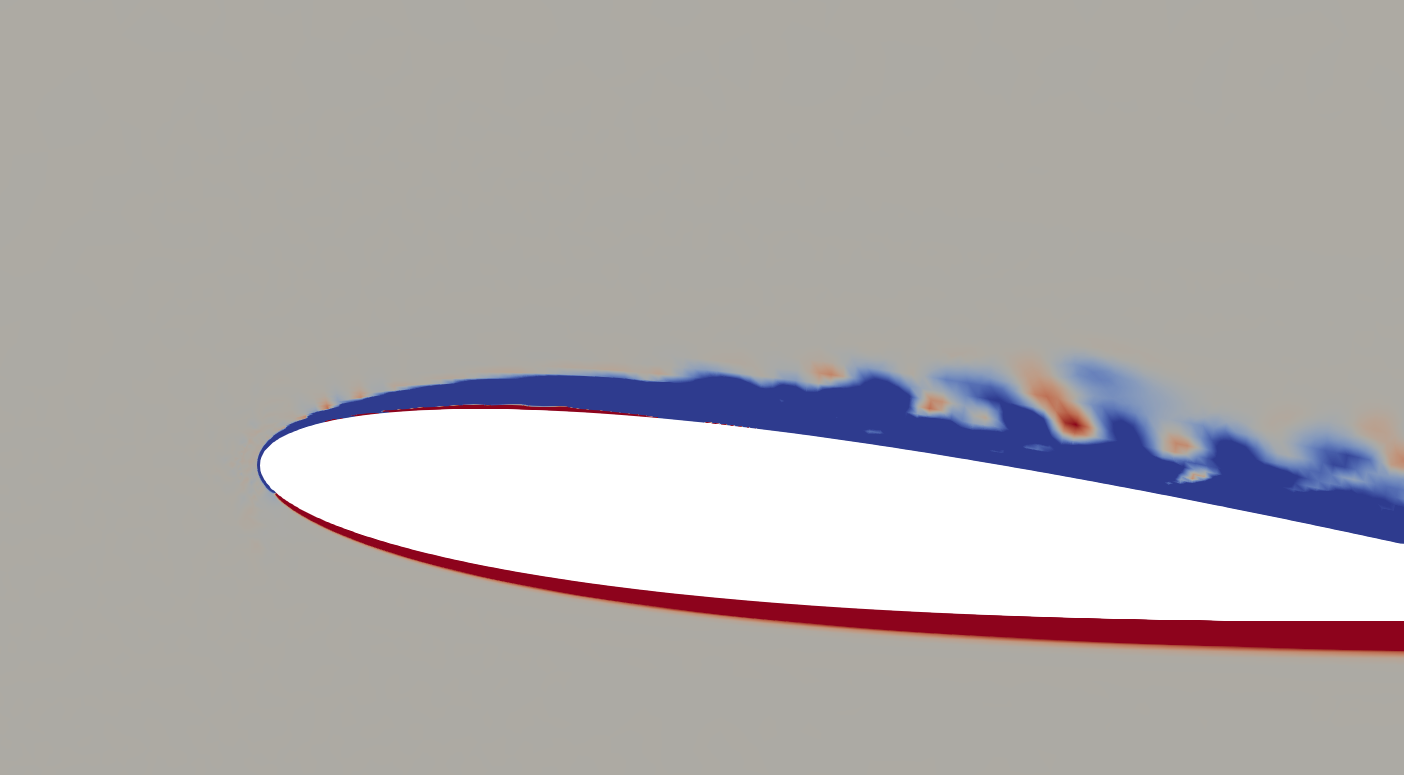
\includegraphics[width=1\textwidth]{figures/zonal_adapt_results/vorticity_plots/v2/Mza1_25/spavg/phase_180.png}
	\caption{Mza1\_25 mesh, $\psi$ = $180^\circ$}
	\label{fig:Mza1_25_sp_psi180}
\end{subfigure}
	\begin{subfigure}[b]{0.475\textwidth}
		\centering
		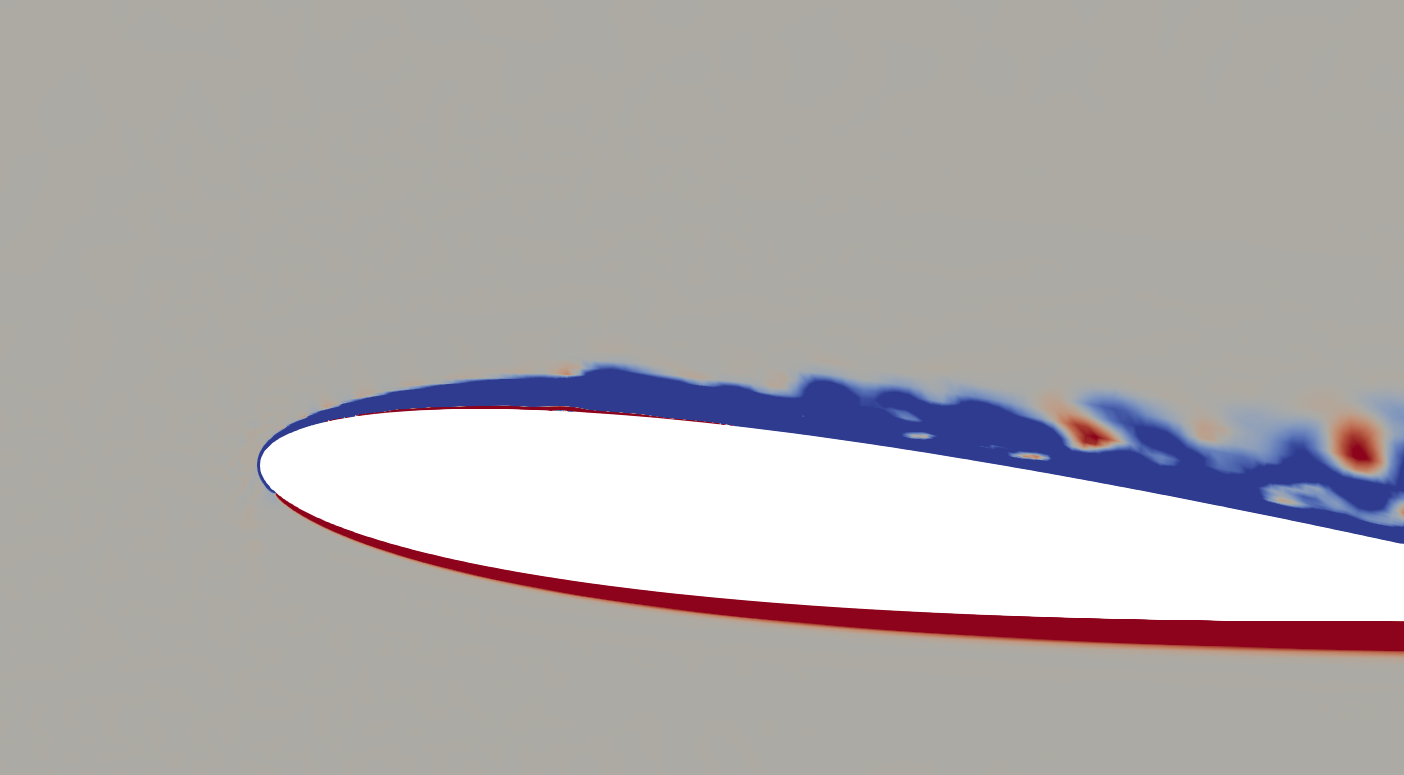
\includegraphics[width=1\textwidth]{figures/zonal_adapt_results/vorticity_plots/v2/Mza1_50/spavg/phase_180.png}
		\caption{Mza1\_50 mesh, $\psi$ = $180^\circ$}
		\label{fig:Mza1_50_sp_psi180}
	\end{subfigure}
%	\begin{subfigure}[b]{0.475\textwidth}
%		\centering
%		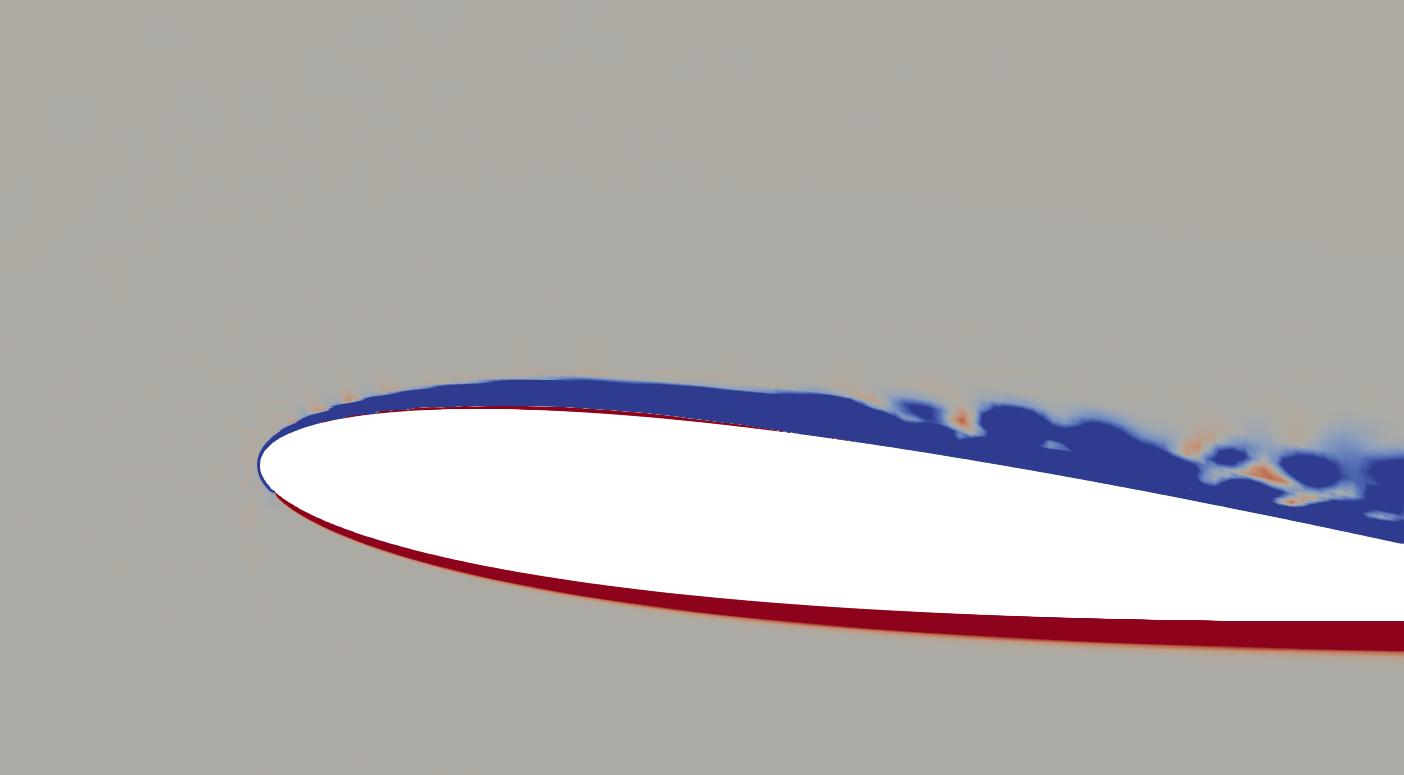
\includegraphics[width=1\textwidth]{figures/zonal_adapt_results/vorticity_plots/v2/Mza1_100/spavg/phase_180.png}
%		\caption{Mza1\_100 mesh, $\psi$ = $180^\circ$}
%		\label{fig:Mza1_100_sp_psi180}
%	\end{subfigure}
%	\begin{subfigure}[b]{0.475\textwidth}
%	\centering
%	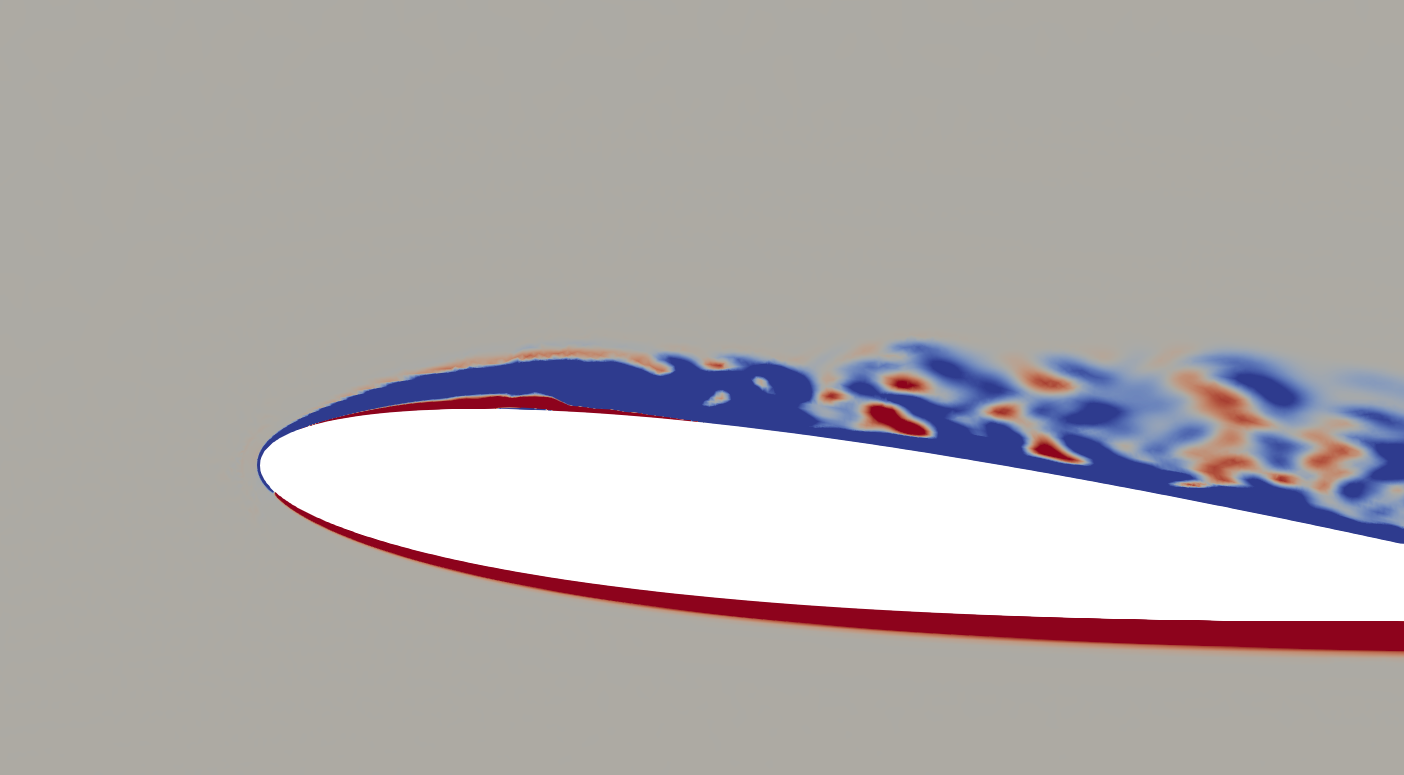
\includegraphics[width=1\textwidth]{figures/zonal_adapt_results/vorticity_plots/v2/Mza2_25/spavg/phase_180.png}
%	\caption{Mza2\_25 mesh, $\psi$ = $180^\circ$}
%	\label{fig:Mza2_25_sp_psi180}
%	\end{subfigure}
	\begin{subfigure}[b]{0.475\textwidth}
		\centering
		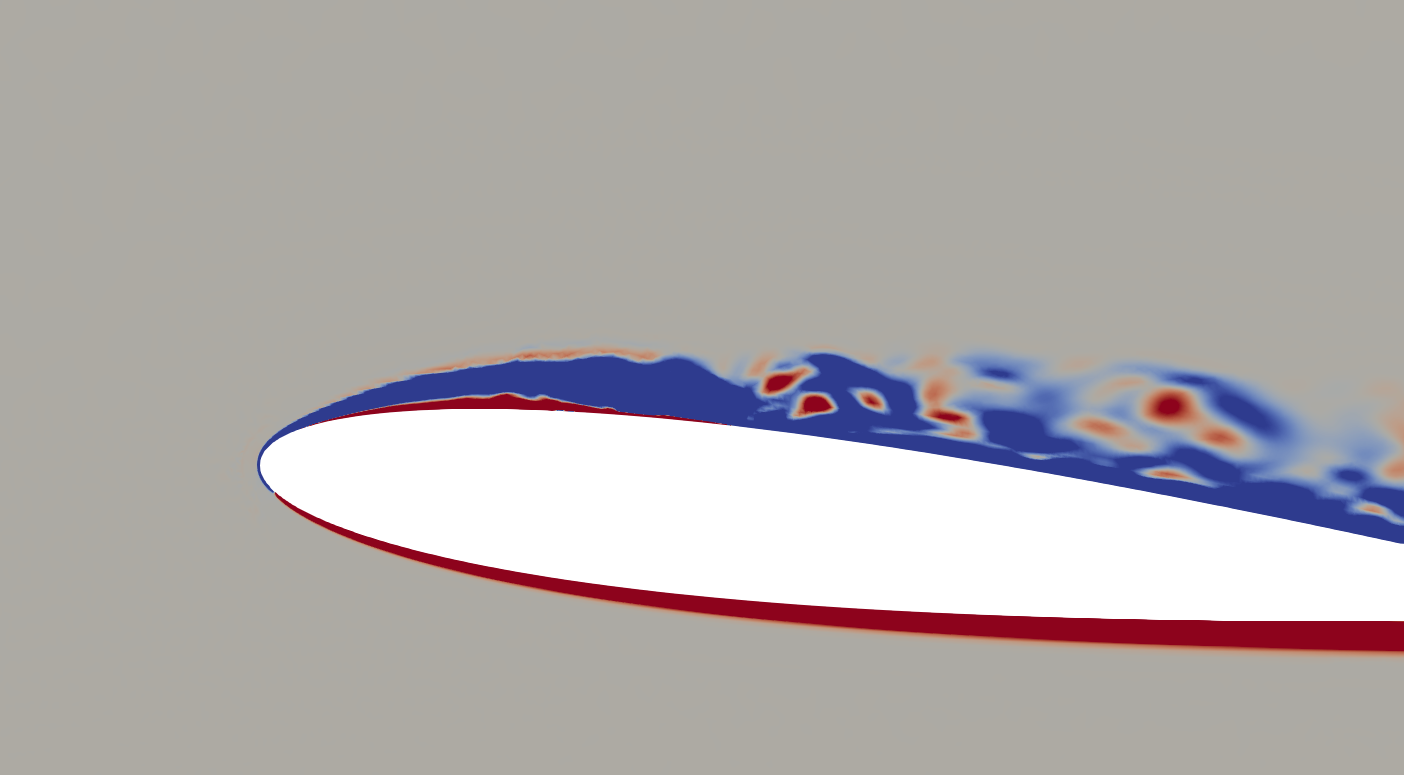
\includegraphics[width=1\textwidth]{figures/zonal_adapt_results/vorticity_plots/v2/Mza2_50/spavg/phase_180.png}
		\caption{Mza2\_50 mesh, $\psi$ = $180^\circ$}
		\label{fig:Mza2_50_sp_psi180}
	\end{subfigure}	
	\begin{subfigure}[b]{0.475\textwidth}
		\centering
		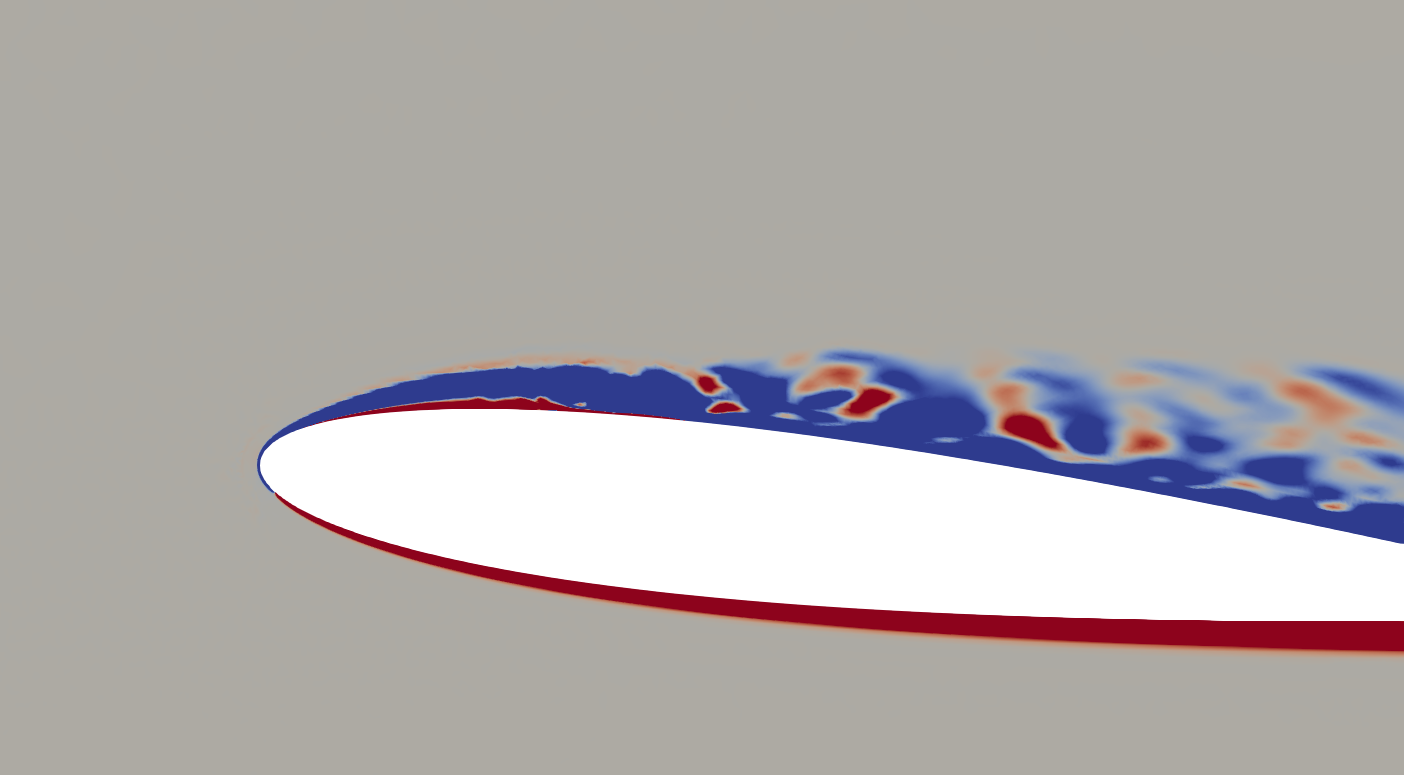
\includegraphics[width=1\textwidth]{figures/zonal_adapt_results/vorticity_plots/v2/Mza2_100/spavg/phase_180.png}
		\caption{Mza2\_100 mesh, $\psi$ = $180^\circ$}
		\label{fig:Mza2_100_sp_psi180}
	\end{subfigure}
	\begin{subfigure}[b]{0.475\textwidth}
	\centering
	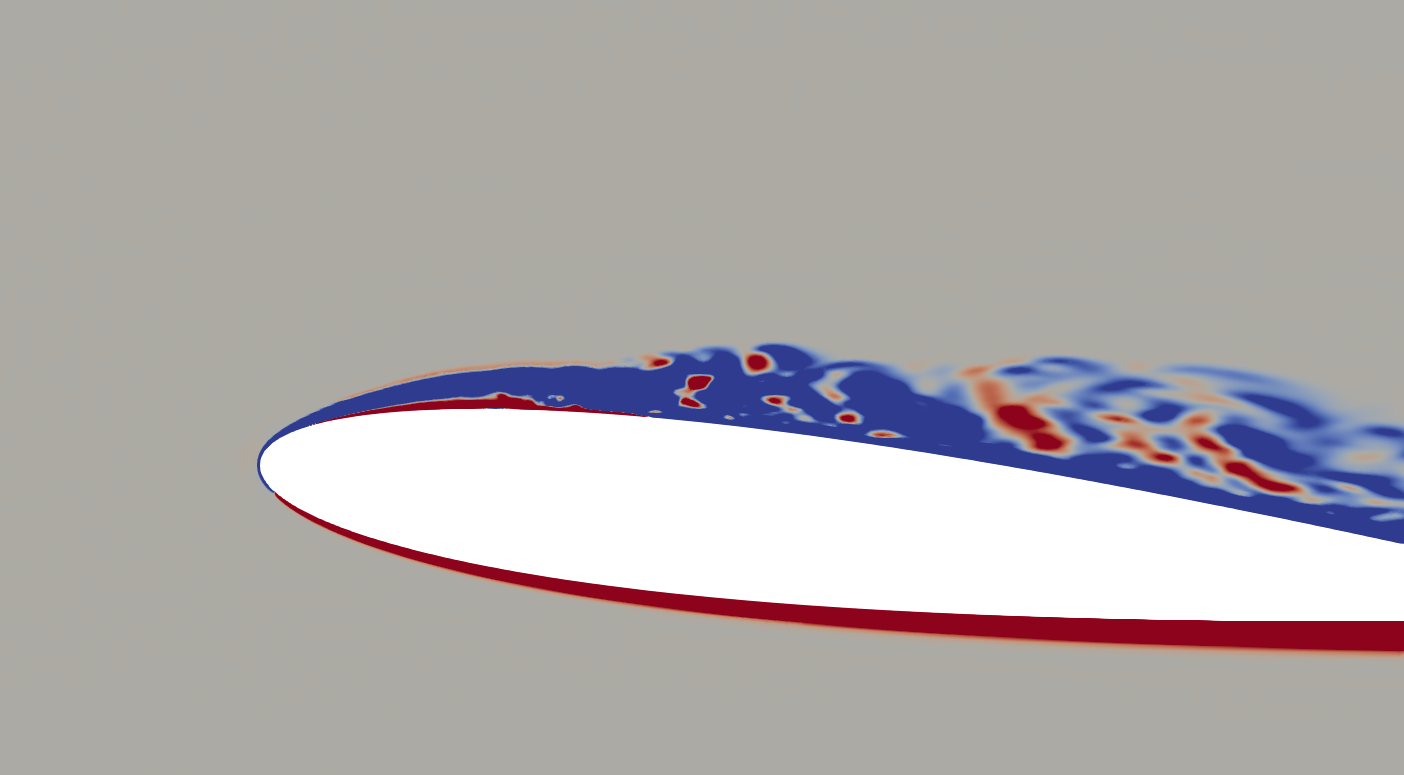
\includegraphics[width=1\textwidth]{figures/zonal_adapt_results/vorticity_plots/v2/Mza3_50/spavg/phase_180.png}
	\caption{Mza3\_50 mesh, $\psi$ = $180^\circ$}
	\label{fig:Mza3_100_sp_psi180}
	\end{subfigure}
	\begin{subfigure}[b]{0.475\textwidth}
		\centering
		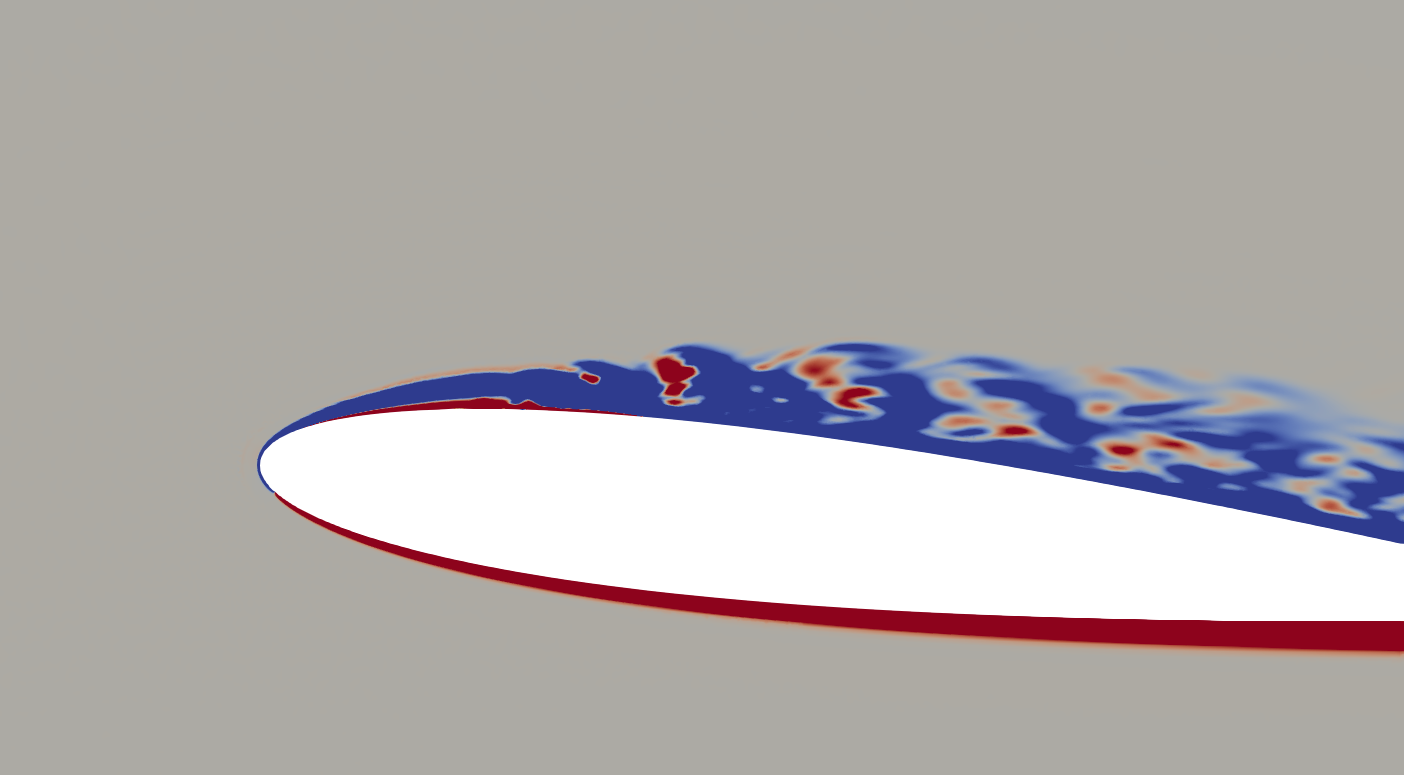
\includegraphics[width=1\textwidth]{figures/zonal_adapt_results/vorticity_plots/v2/Mza3_100/spavg/phase_180.png}
		\caption{Mza3\_100 mesh, $\psi$ = $180^\circ$}
		\label{fig:Mza3_100_sp_psi180}
	\end{subfigure}
	\caption{Spanwise vorticity comparison at $\psi$ = $180^\circ$ for different meshes}
	\label{fig:vorticity_zonal_180}
\end{figure}

%%=====================================
%% Phase = 210
%%=====================================


\begin{figure}[H]
	\centering
	\begin{center}
		\begin{subfigure}[b]{0.475\textwidth}
		\centering
		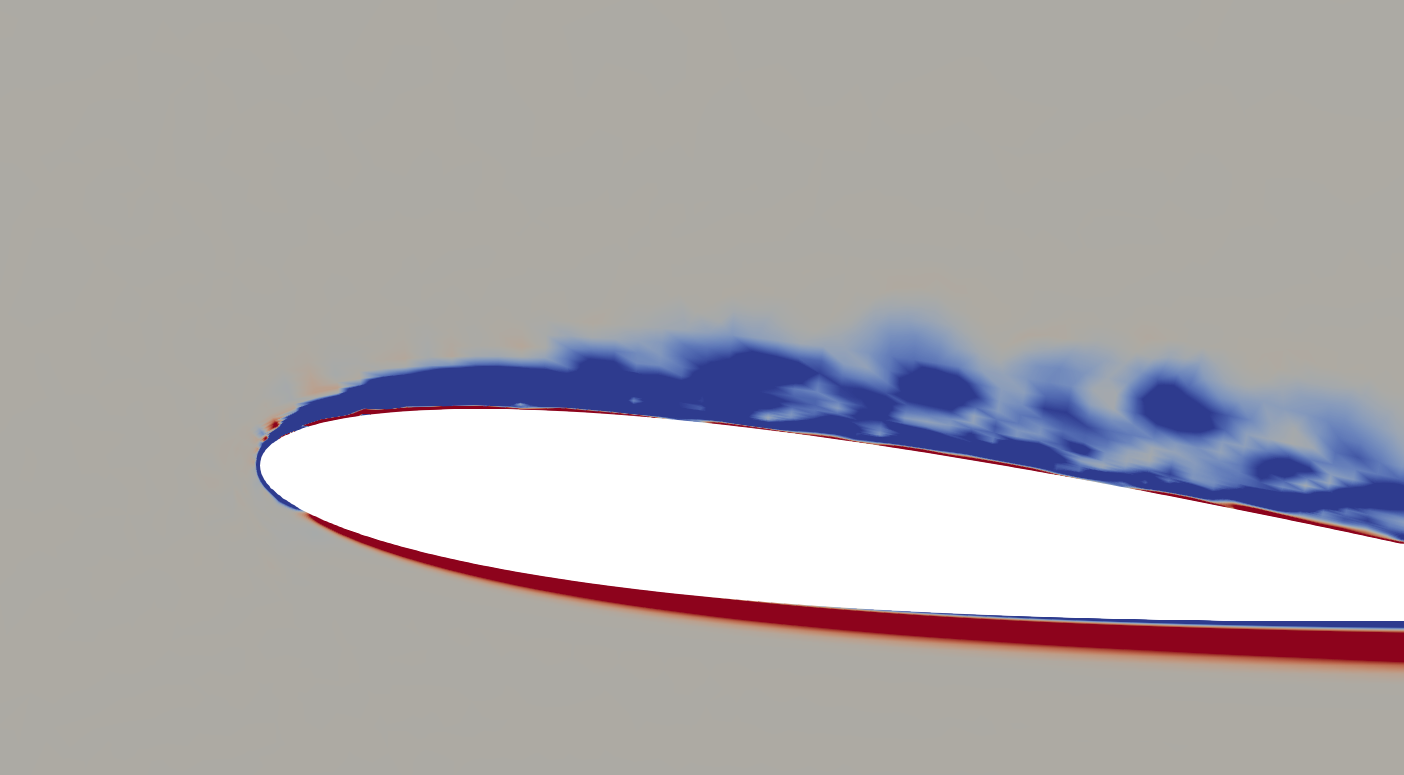
\includegraphics[width=1\textwidth]{figures/zonal_adapt_results/vorticity_plots/v2/M0/spavg/phase_210.png}
		\caption{M0 mesh, $\psi$ = $210^\circ$}
		\label{fig:M0_sp_psi210}
		\end{subfigure}
	\end{center}
	\begin{subfigure}[b]{0.475\textwidth}
	\centering
	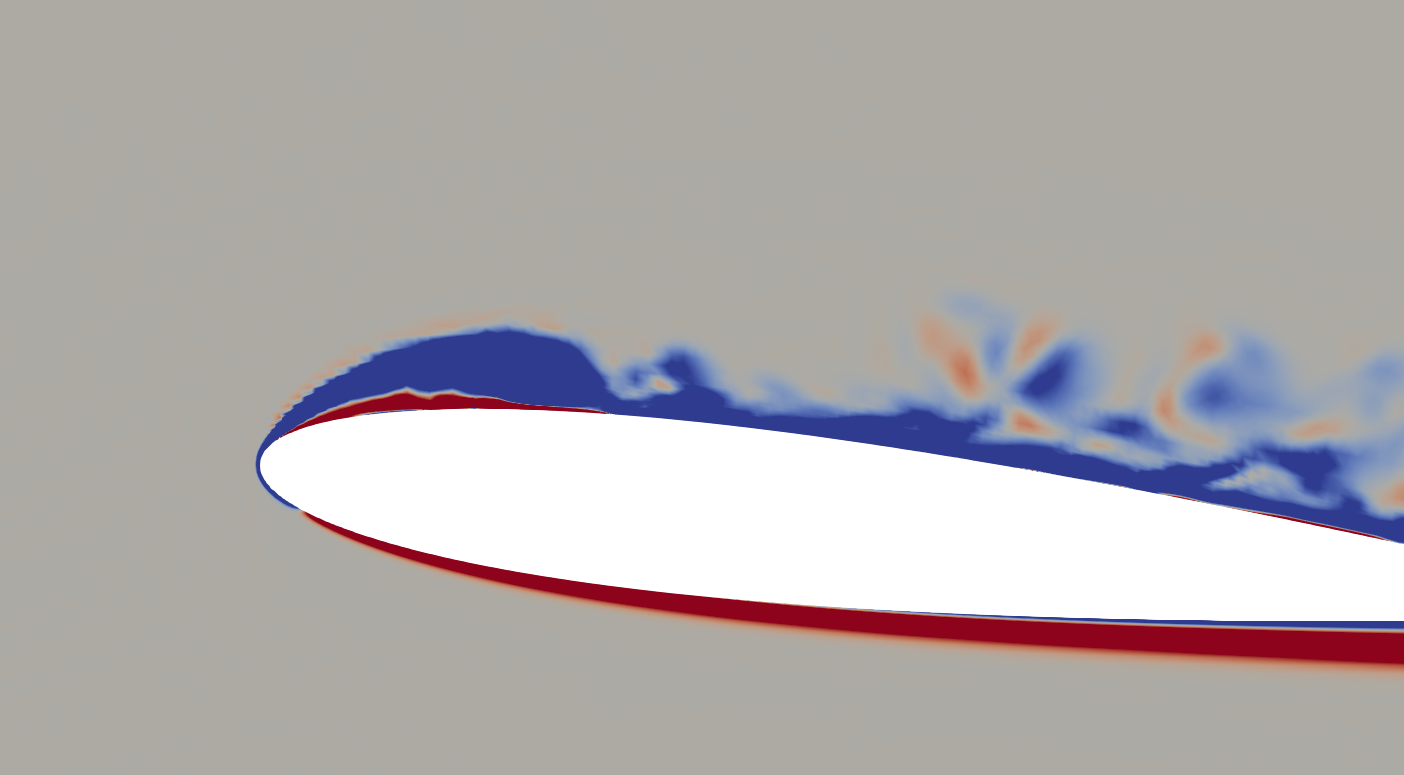
\includegraphics[width=1\textwidth]{figures/zonal_adapt_results/vorticity_plots/v2/Mza1_25/spavg/phase_210.png}
	\caption{Mza1\_25 mesh, $\psi$ = $210^\circ$}
	\label{fig:Mza1_25_sp_psi210}
	\end{subfigure}
	\begin{subfigure}[b]{0.475\textwidth}
		\centering
		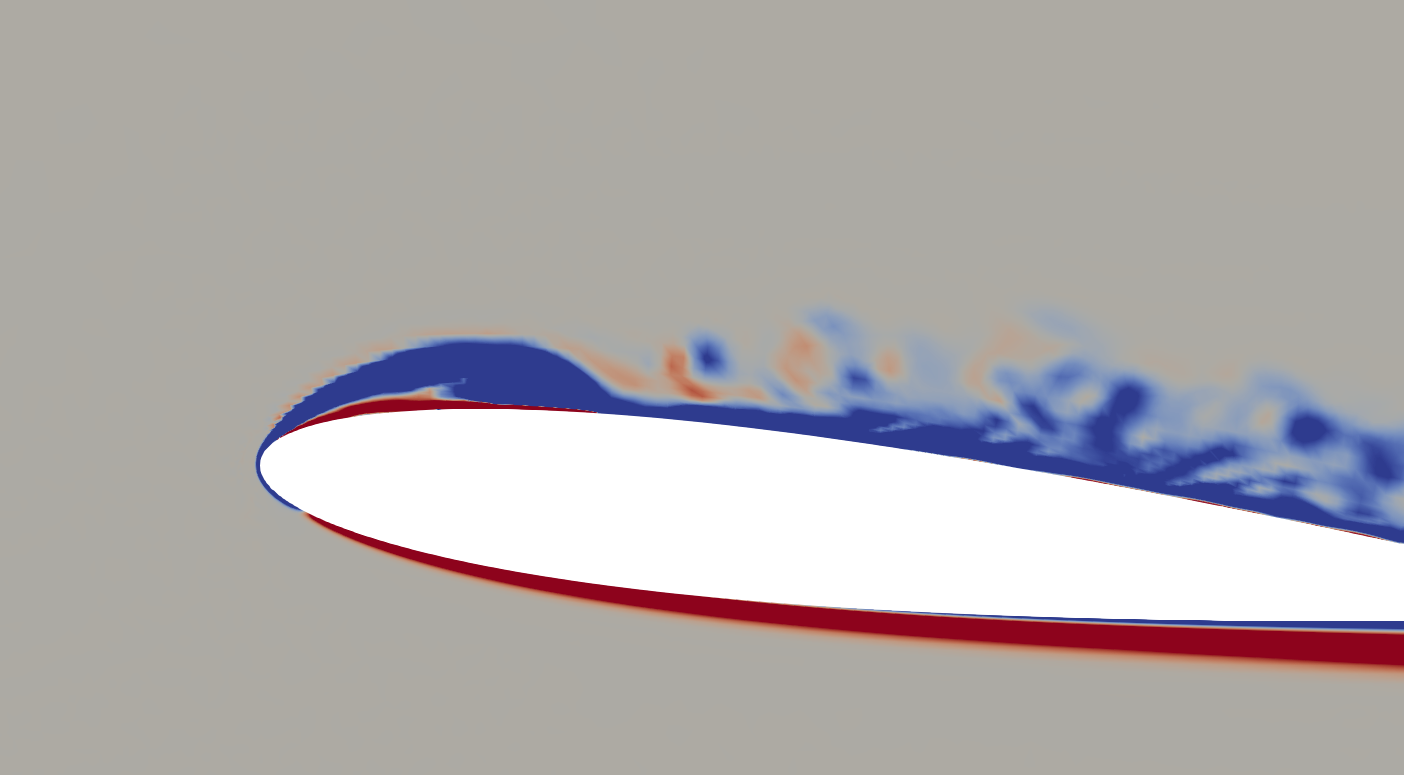
\includegraphics[width=1\textwidth]{figures/zonal_adapt_results/vorticity_plots/v2/Mza1_50/spavg/phase_210.png}
		\caption{Mza1\_50 mesh, $\psi$ = $210^\circ$}
		\label{fig:Mza1_50_sp_psi210}
	\end{subfigure}
%	\begin{subfigure}[b]{0.475\textwidth}
%		\centering
%		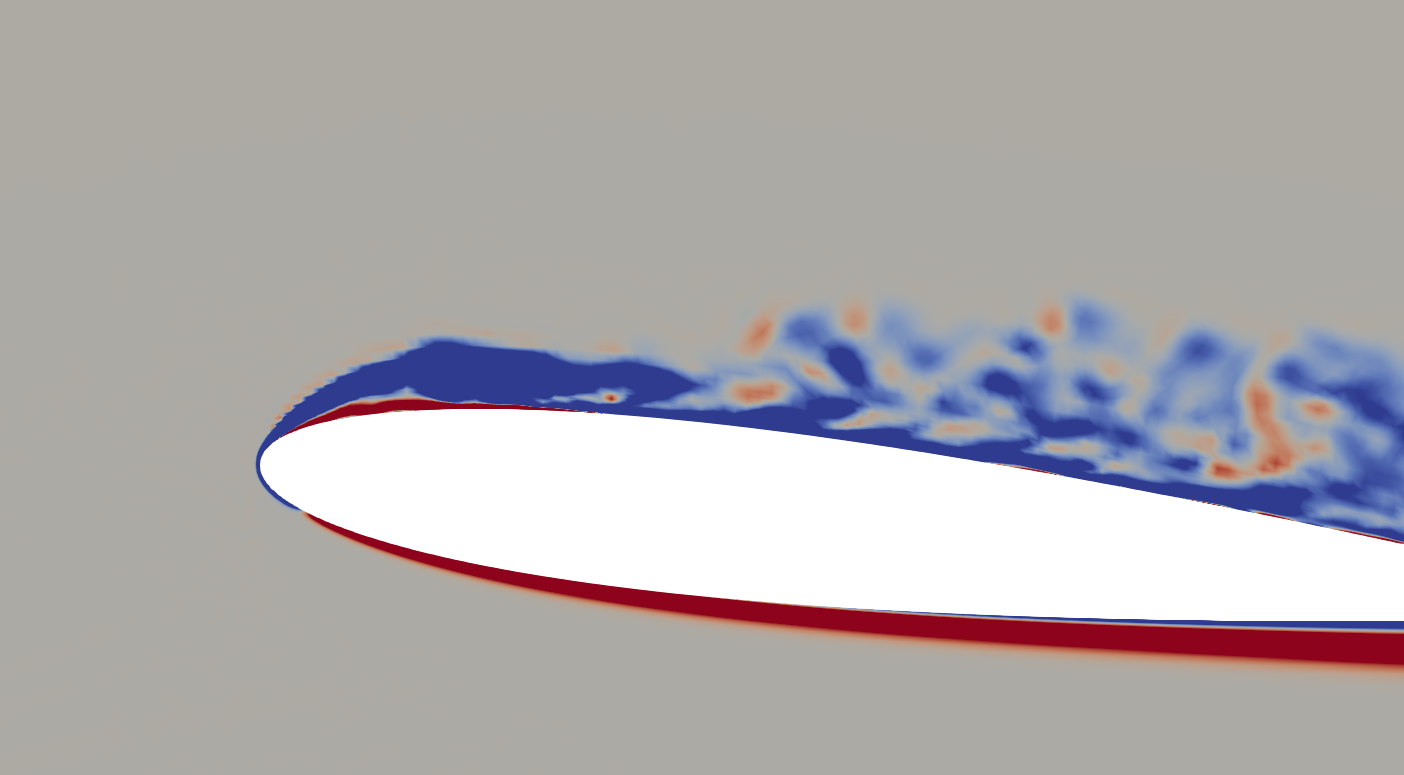
\includegraphics[width=1\textwidth]{figures/zonal_adapt_results/vorticity_plots/v2/Mza1_100/spavg/phase_210.png}
%		\caption{Mza1\_100 mesh, $\psi$ = $210^\circ$}
%		\label{fig:Mza1_100_sp_psi210}
%	\end{subfigure}
%	\begin{subfigure}[b]{0.475\textwidth}
%	\centering
%	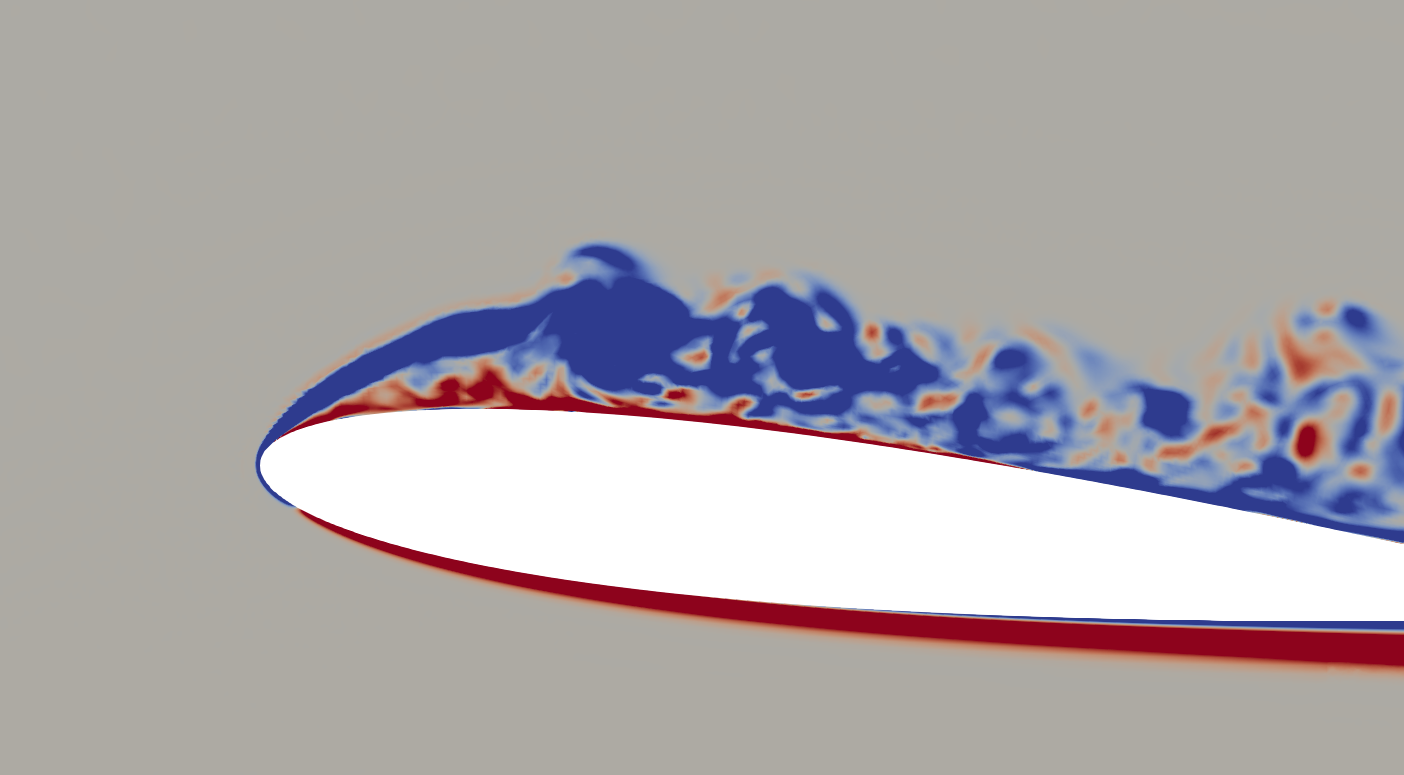
\includegraphics[width=1\textwidth]{figures/zonal_adapt_results/vorticity_plots/v2/Mza2_25/spavg/phase_210.png}
%	\caption{Mza2\_25 mesh, $\psi$ = $210^\circ$}
%	\label{fig:Mza2_25_sp_psi210}
%	\end{subfigure}	
	\begin{subfigure}[b]{0.475\textwidth}
		\centering
		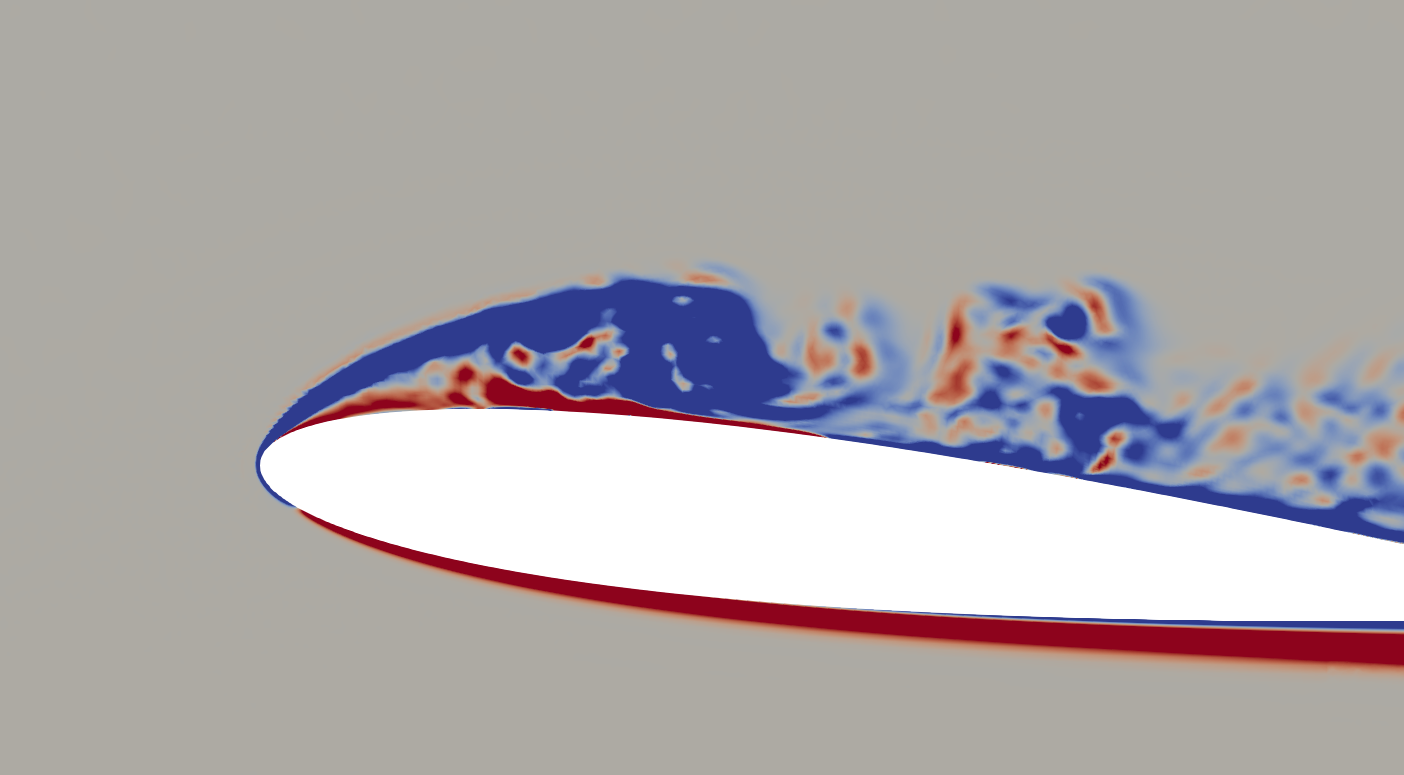
\includegraphics[width=1\textwidth]{figures/zonal_adapt_results/vorticity_plots/v2/Mza2_50/spavg/phase_210.png}
		\caption{Mza2\_50 mesh, $\psi$ = $210^\circ$}
		\label{fig:Mza2_50_sp_psi210}
	\end{subfigure}	
	\begin{subfigure}[b]{0.475\textwidth}
		\centering
		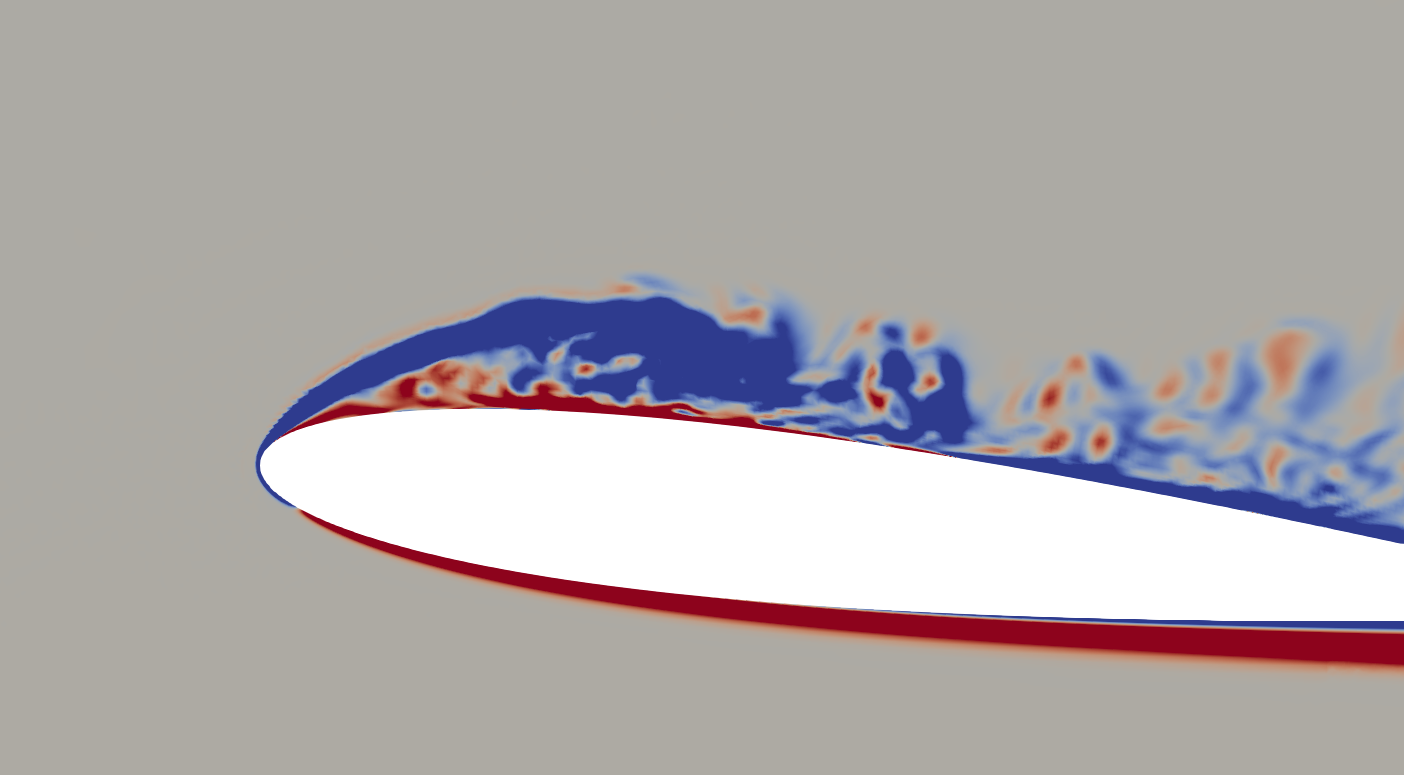
\includegraphics[width=1\textwidth]{figures/zonal_adapt_results/vorticity_plots/v2/Mza2_100/spavg/phase_210.png}
		\caption{Mza2\_100 mesh, $\psi$ = $210^\circ$}
		\label{fig:Mza2_100_sp_psi210}
	\end{subfigure}
	\begin{subfigure}[b]{0.475\textwidth}
	\centering
	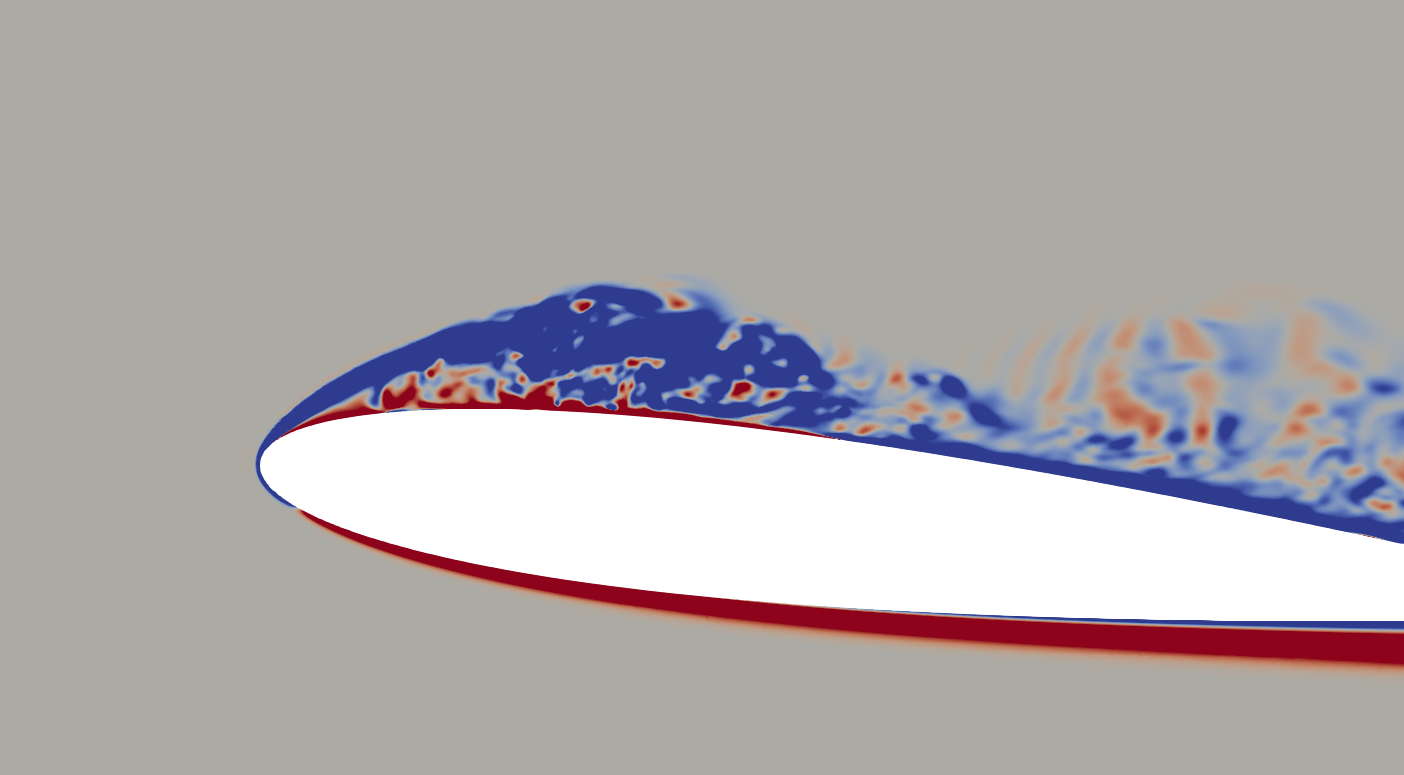
\includegraphics[width=1\textwidth]{figures/zonal_adapt_results/vorticity_plots/v2/Mza3_50/spavg/phase_210.png}
	\caption{Mza3\_50 mesh, $\psi$ = $210^\circ$}
	\label{fig:Mza3_50_sp_psi210}
\end{subfigure}
	\begin{subfigure}[b]{0.475\textwidth}
		\centering
		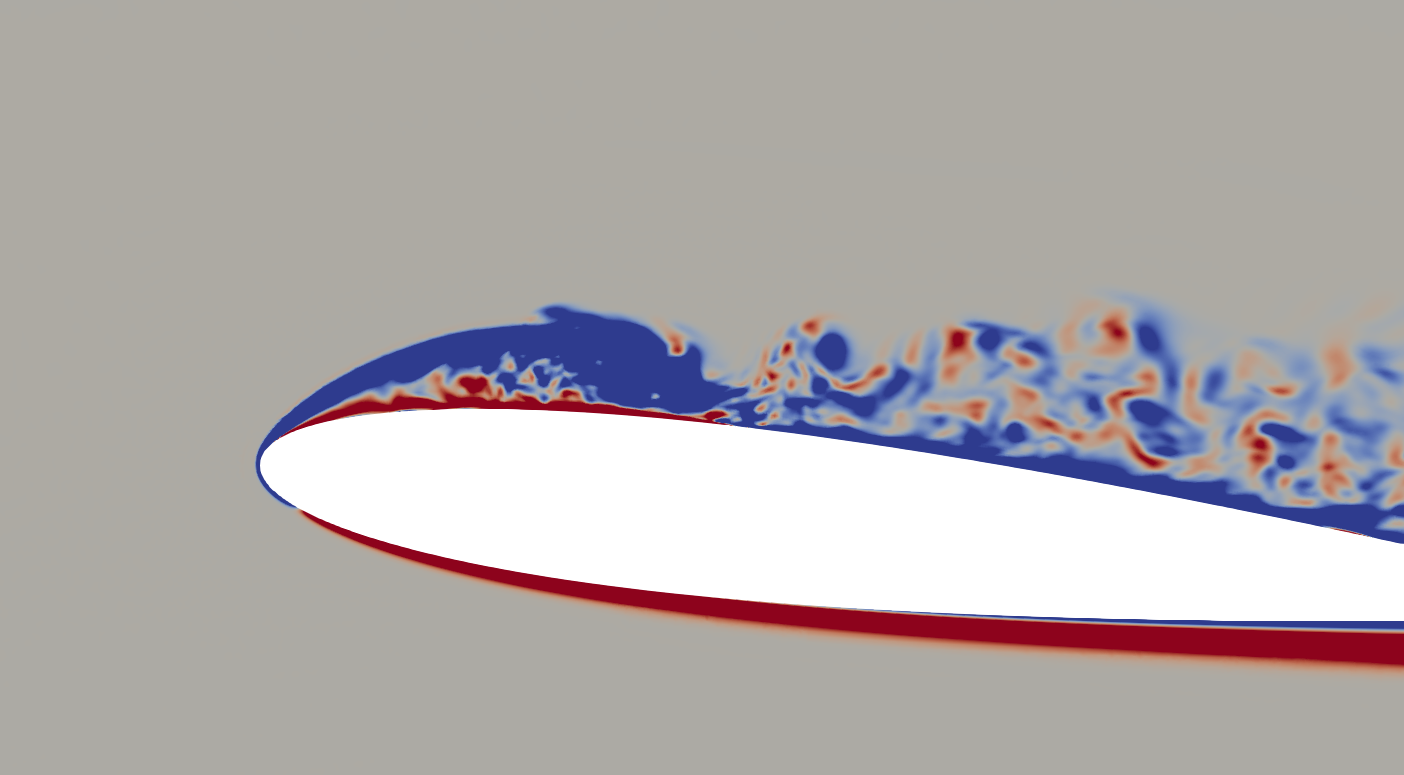
\includegraphics[width=1\textwidth]{figures/zonal_adapt_results/vorticity_plots/v2/Mza3_100/spavg/phase_210.png}
		\caption{Mza3\_100 mesh, $\psi$ = $210^\circ$}
		\label{fig:Mza3_100_sp_psi210}
	\end{subfigure}
	\caption{Spanwise vorticity comparison at $\psi$ = $210^\circ$ for different meshes}
	\label{fig:vorticity_zonal_210}
\end{figure}

%%=====================================
%% Phase = 240
%%=====================================


\begin{figure}[H]
	\centering
	\begin{center}
		\begin{subfigure}[b]{0.475\textwidth}
		\centering
		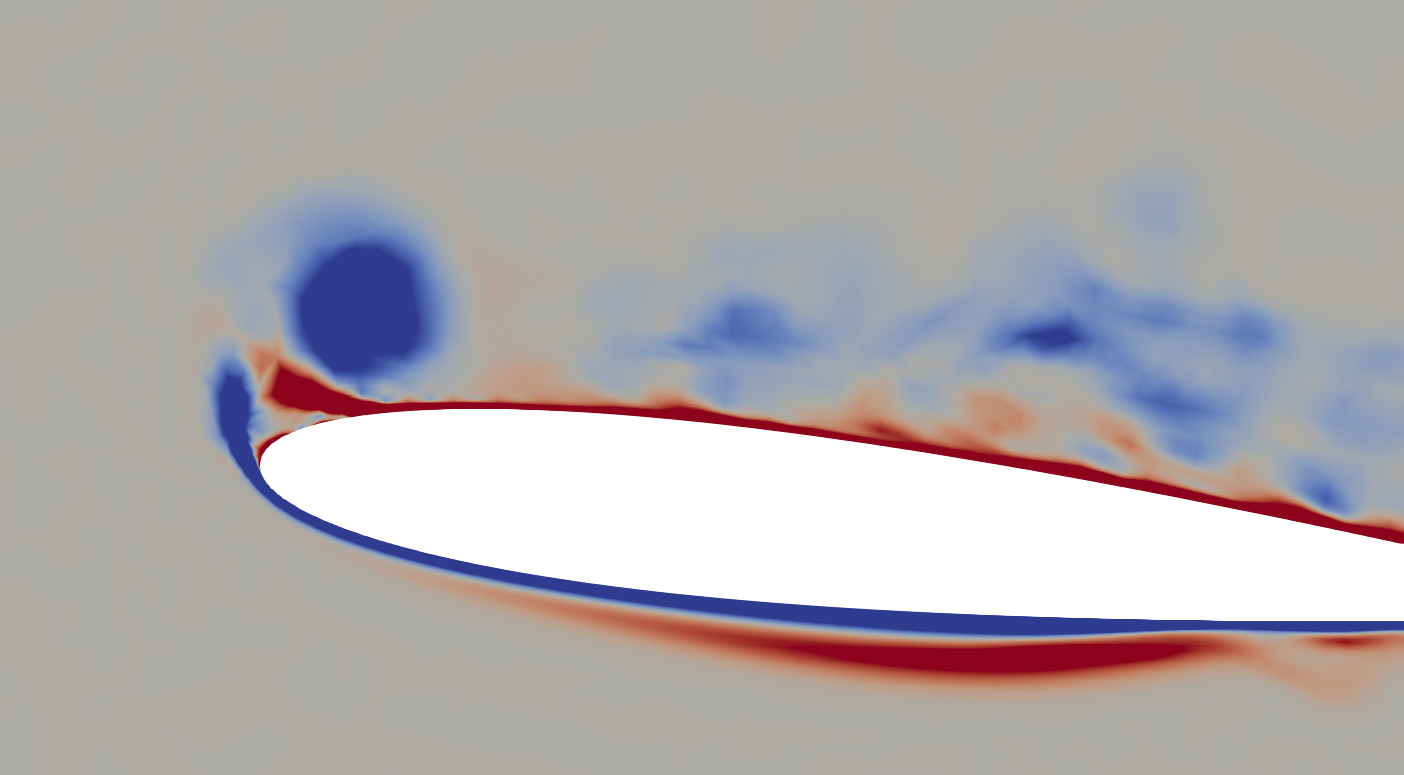
\includegraphics[width=1\textwidth]{figures/zonal_adapt_results/vorticity_plots/v2/M0/spavg/phase_240.png}
		\caption{M0 mesh, $\psi$ = $240^\circ$}
		\label{fig:M0_sp_psi240}
		\end{subfigure}
	\end{center}
	\begin{subfigure}[b]{0.475\textwidth}
		\centering
		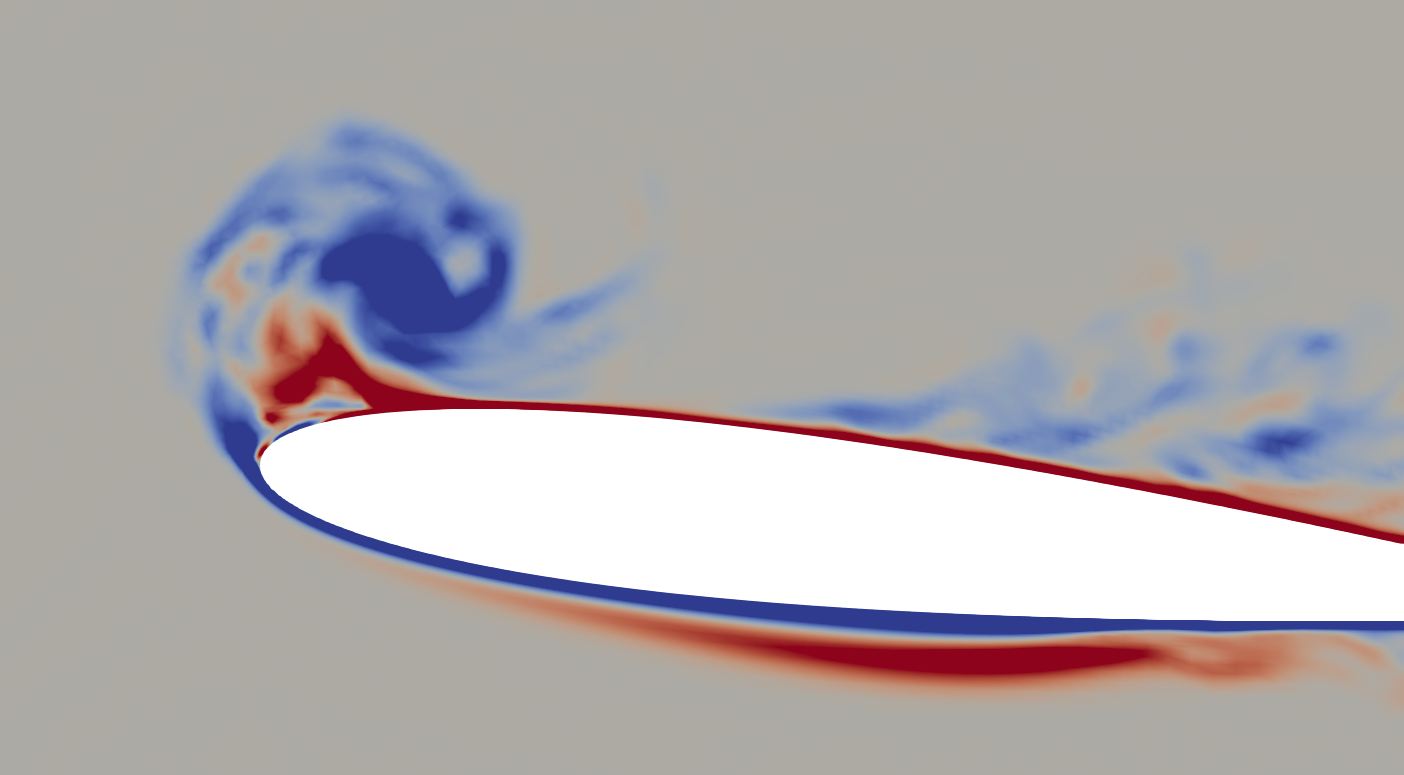
\includegraphics[width=1\textwidth]{figures/zonal_adapt_results/vorticity_plots/v2/Mza1_25/spavg/phase_240.png}
		\caption{Mza1\_25 mesh, $\psi$ = $240^\circ$}
		\label{fig:Mza1_25_sp_psi240}
	\end{subfigure}
	\begin{subfigure}[b]{0.475\textwidth}
	\centering
	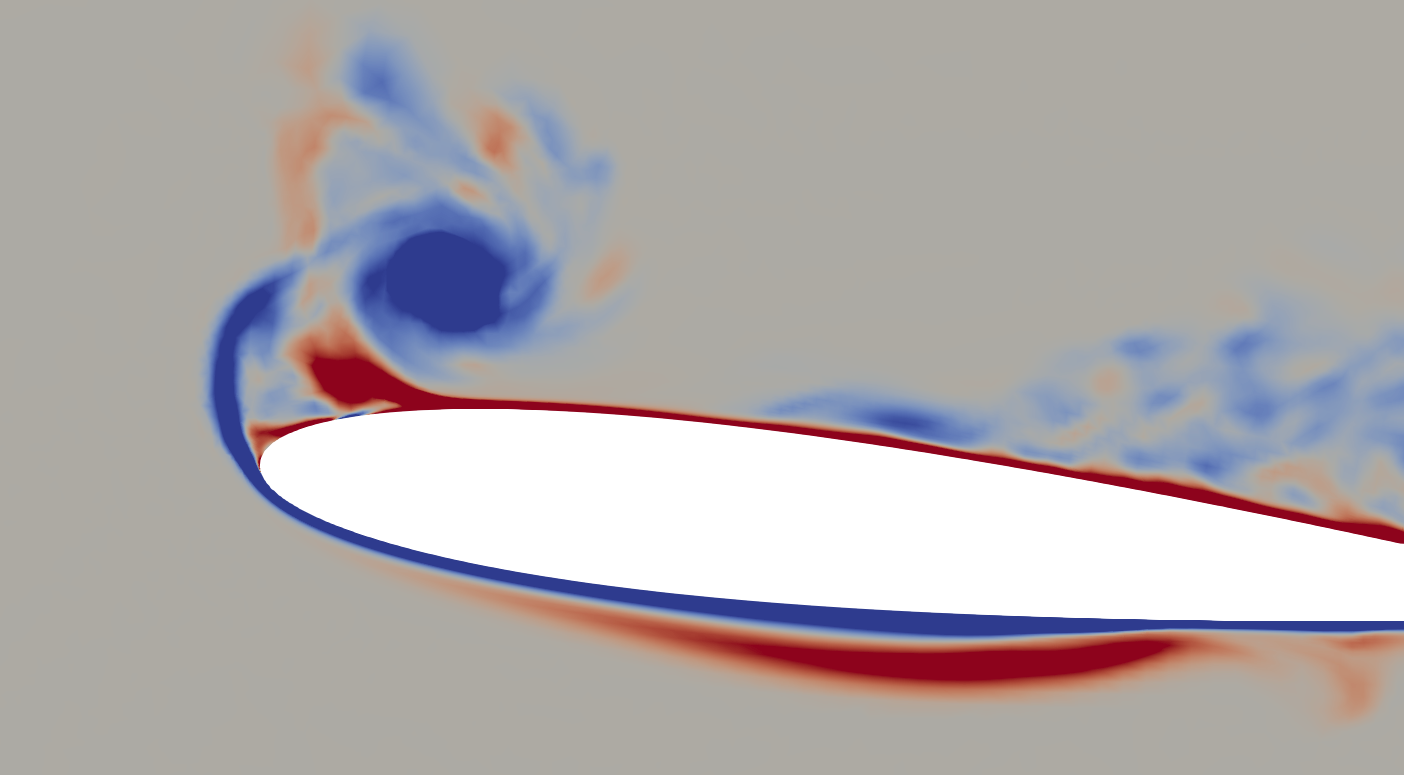
\includegraphics[width=1\textwidth]{figures/zonal_adapt_results/vorticity_plots/v2/Mza1_50/spavg/phase_240.png}
	\caption{Mza1\_50 mesh, $\psi$ = $240^\circ$}
	\label{fig:Mza1_50_sp_psi240}
	\end{subfigure}
	\begin{subfigure}[b]{0.475\textwidth}
		\centering
		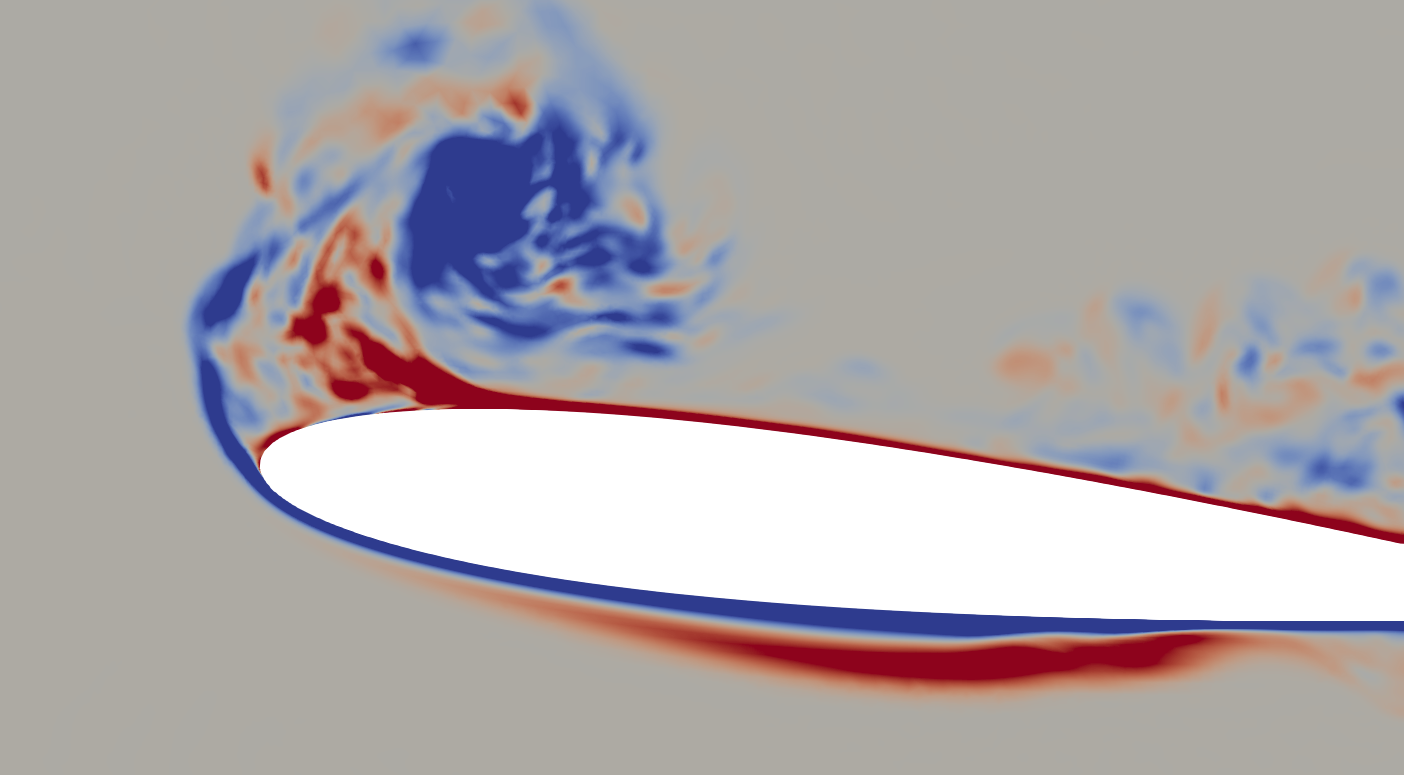
\includegraphics[width=1\textwidth]{figures/zonal_adapt_results/vorticity_plots/v2/Mza2_50/spavg/phase_240.png}
		\caption{Mza2\_50 mesh, $\psi$ = $240^\circ$}
		\label{fig:Mza2_50_sp_psi240}
	\end{subfigure}
%	\begin{subfigure}[b]{0.475\textwidth}
%		\centering
%		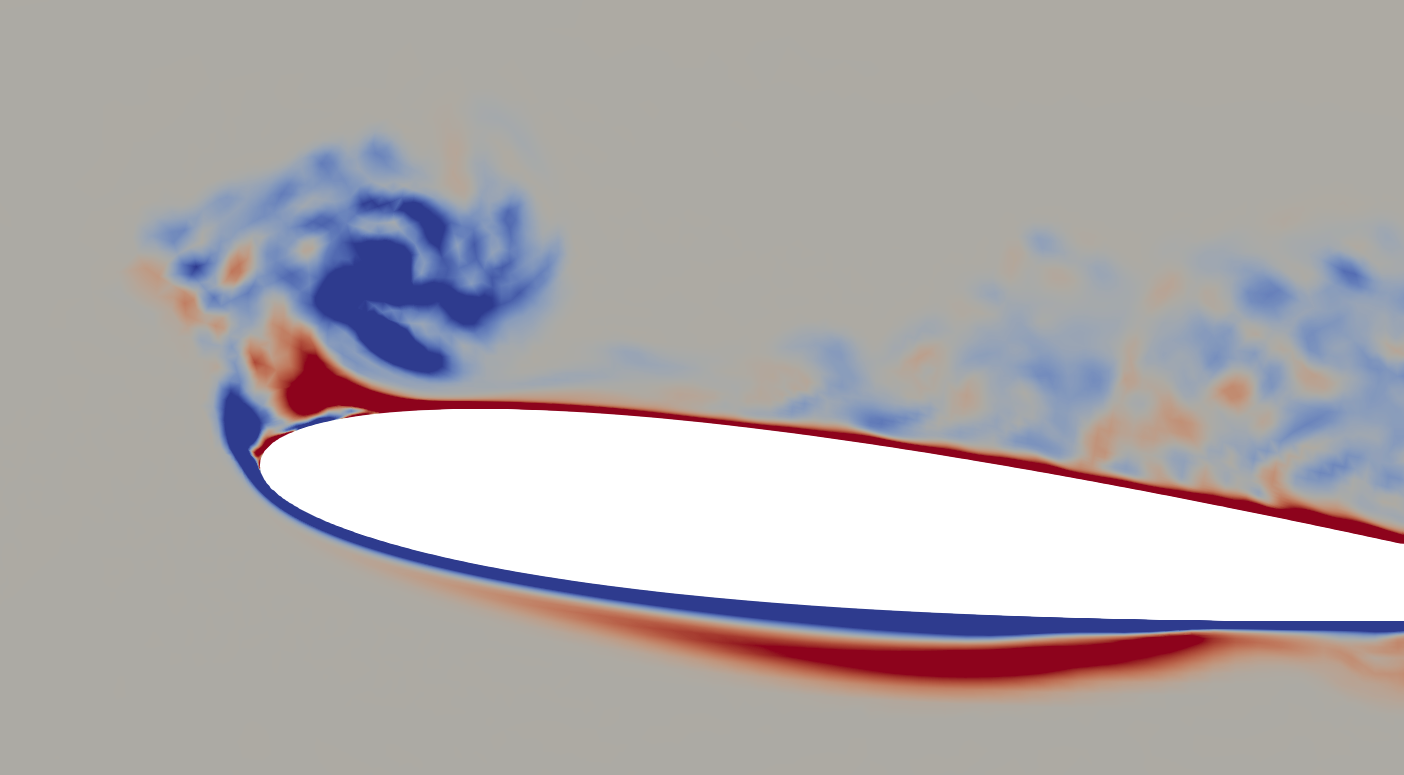
\includegraphics[width=1\textwidth]{figures/zonal_adapt_results/vorticity_plots/v2/Mza1_100/spavg/phase_240.png}
%		\caption{Mza1\_100 mesh, $\psi$ = $240^\circ$}
%		\label{fig:Mza1_100_sp_psi240}
%	\end{subfigure}
%	\begin{subfigure}[b]{0.475\textwidth}
%	\centering
%	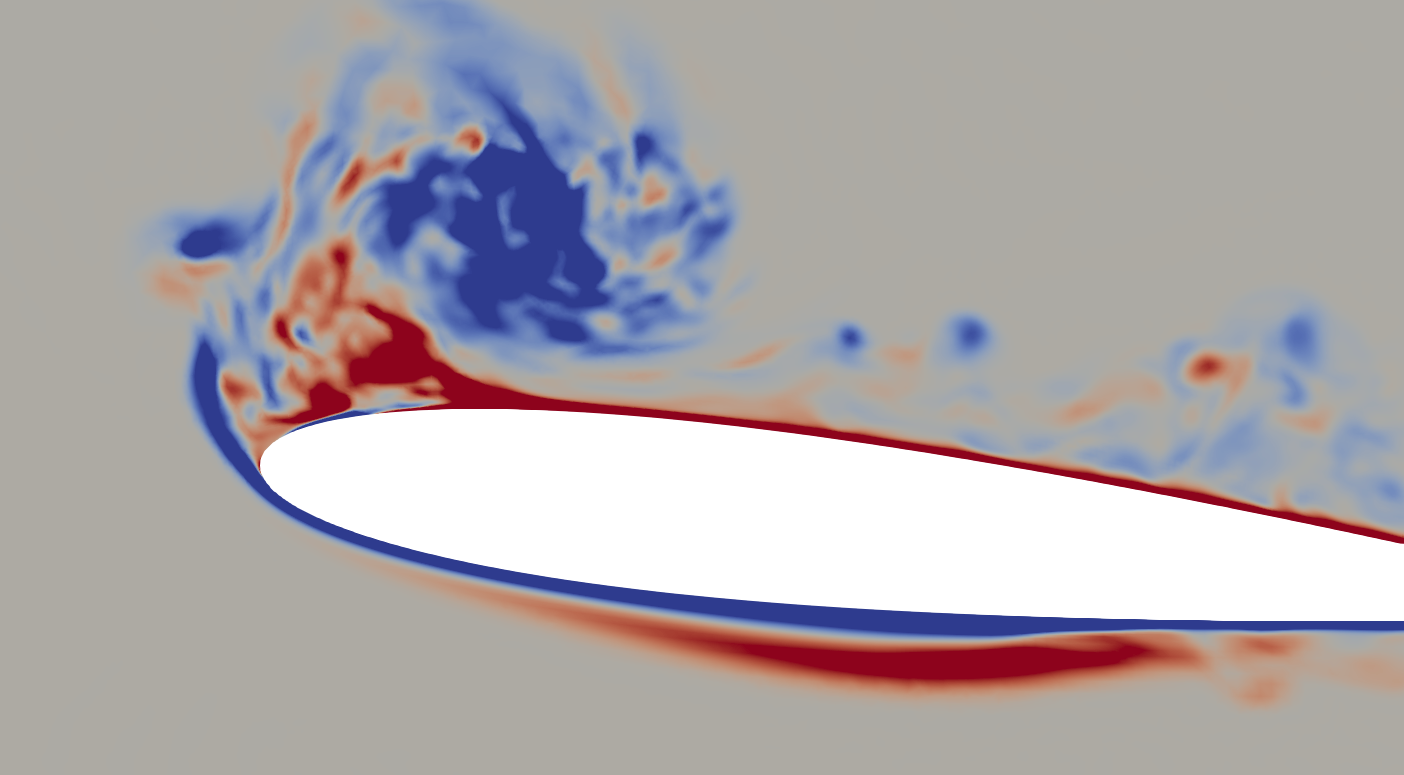
\includegraphics[width=1\textwidth]{figures/zonal_adapt_results/vorticity_plots/v2/Mza2_25/spavg/phase_240.png}
%	\caption{Mza2\_25 mesh, $\psi$ = $240^\circ$}
%	\label{fig:Mza2_25_sp_psi240}
%	\end{subfigure}	
%	\begin{subfigure}[b]{0.475\textwidth}
%		\centering
%		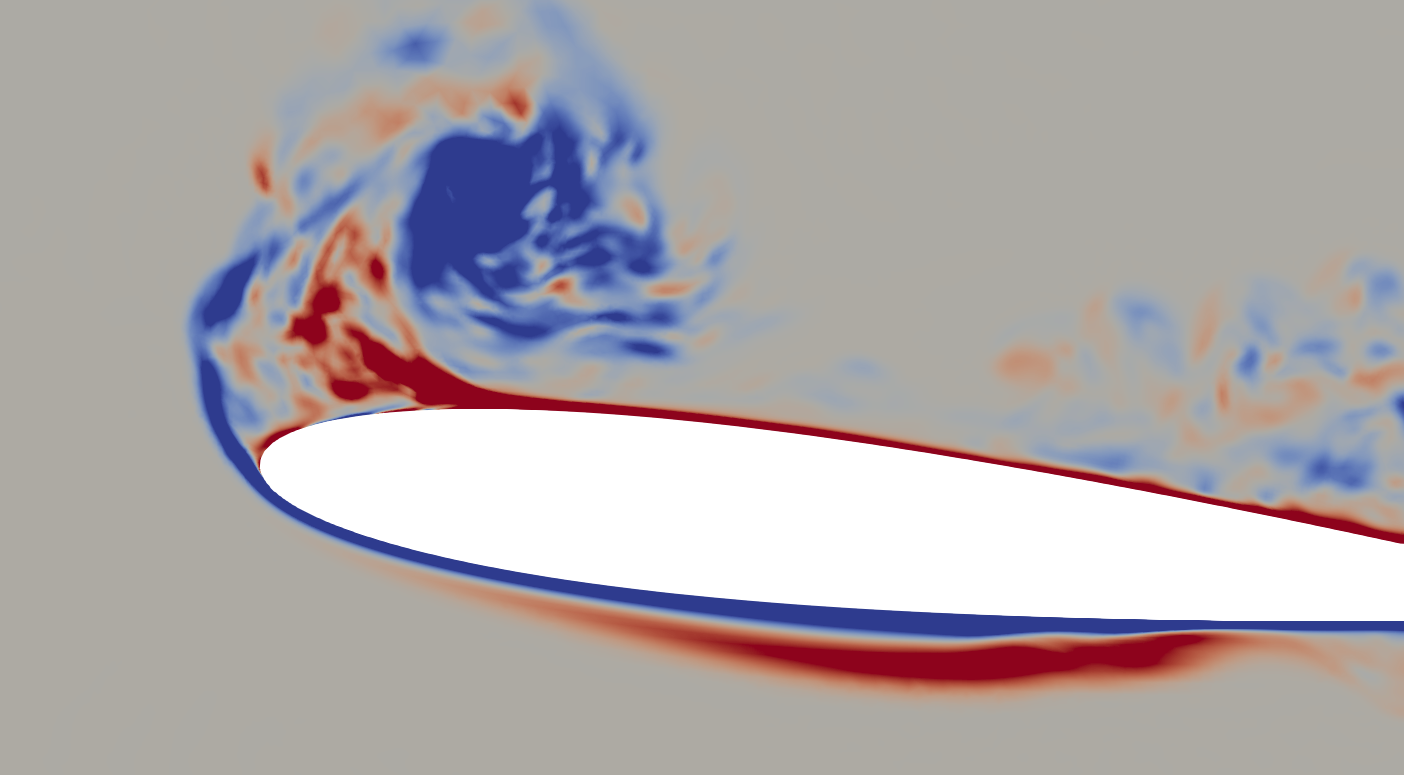
\includegraphics[width=1\textwidth]{figures/zonal_adapt_results/vorticity_plots/v2/Mza2_50/spavg/phase_240.png}
%		\caption{Mza2\_50 mesh, $\psi$ = $240^\circ$}
%		\label{fig:Mza2_50_sp_psi240}
%	\end{subfigure}	
	\begin{subfigure}[b]{0.475\textwidth}
		\centering
		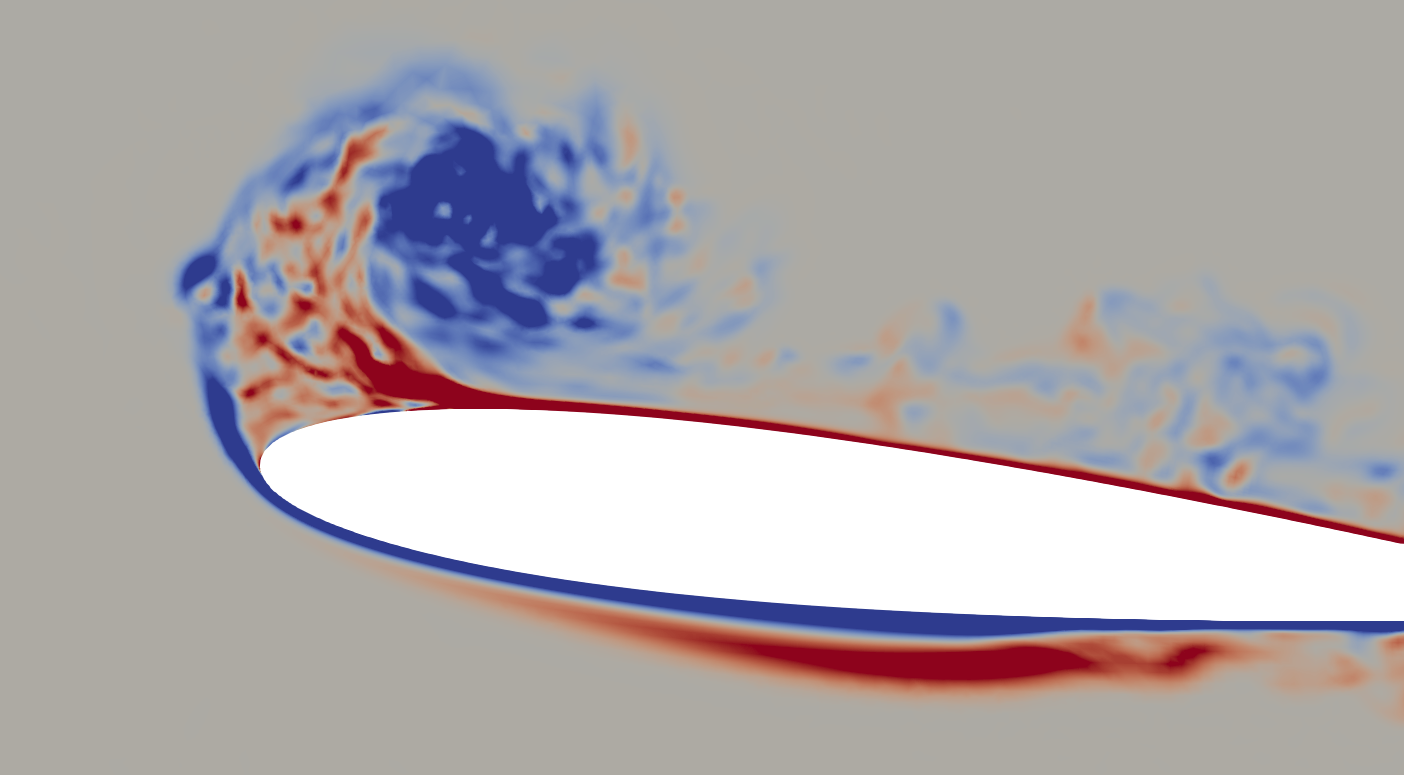
\includegraphics[width=1\textwidth]{figures/zonal_adapt_results/vorticity_plots/v2/Mza2_100/spavg/phase_240.png}
		\caption{Mza2\_100 mesh, $\psi$ = $240^\circ$}
		\label{fig:Mza2_100_sp_psi240}
	\end{subfigure}
	\begin{subfigure}[b]{0.475\textwidth}
	\centering
	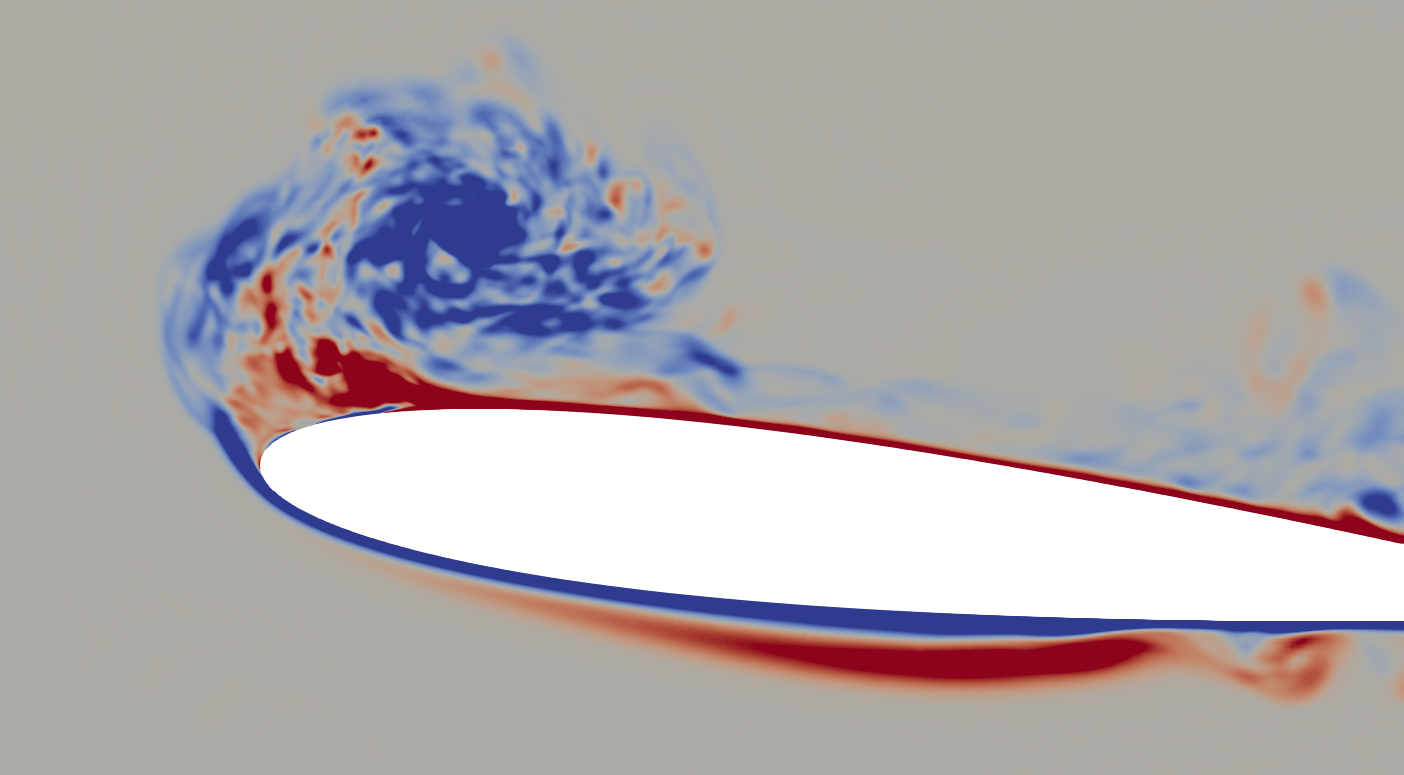
\includegraphics[width=1\textwidth]{figures/zonal_adapt_results/vorticity_plots/v2/Mza3_50/spavg/phase_240.png}
	\caption{Mza3\_50 mesh, $\psi$ = $240^\circ$}
	\label{fig:Mza3_100_sp_psi240}
\end{subfigure}
	\begin{subfigure}[b]{0.475\textwidth}
		\centering
		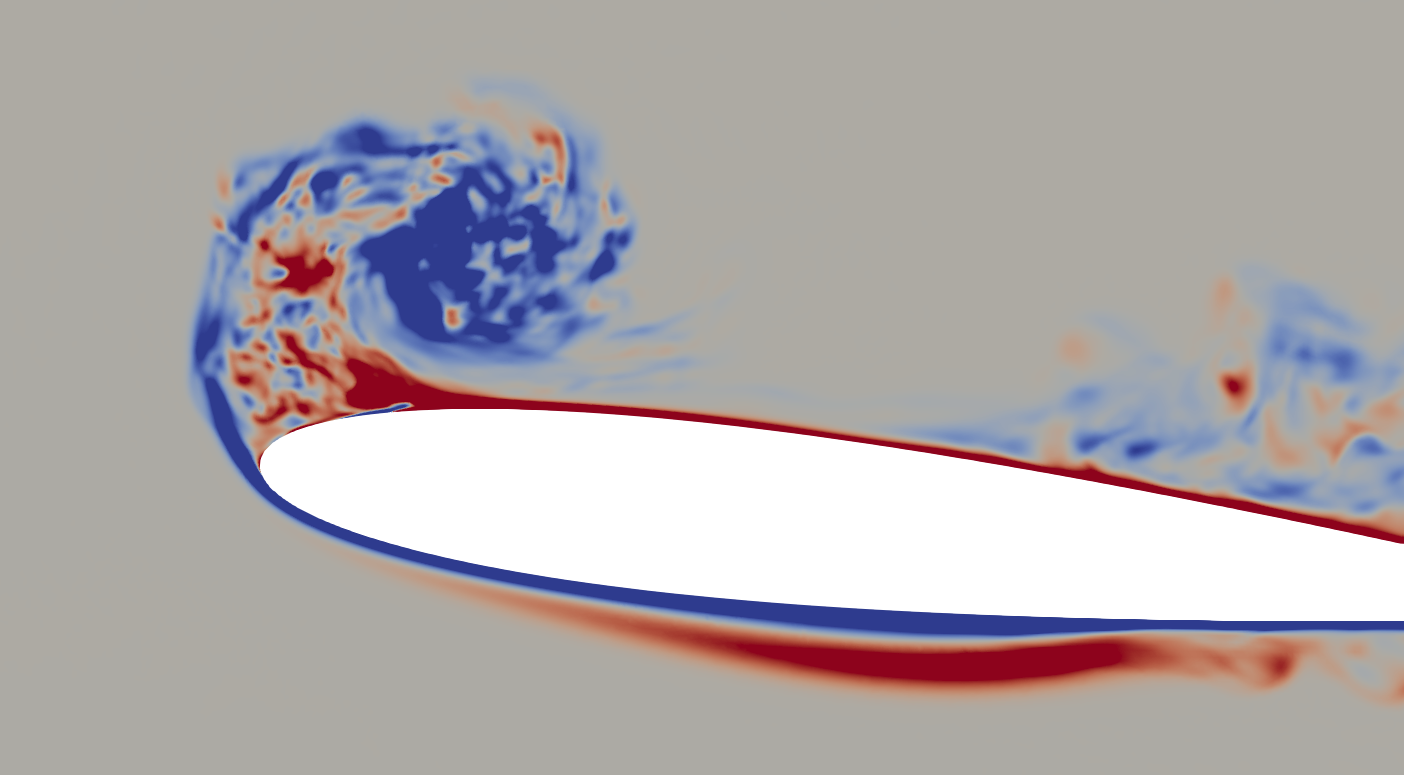
\includegraphics[width=1\textwidth]{figures/zonal_adapt_results/vorticity_plots/v2/Mza3_100/spavg/phase_240.png}
		\caption{Mza3\_100 mesh, $\psi$ = $240^\circ$}
		\label{fig:Mza3_100_sp_psi240}
	\end{subfigure}
	\caption{Spanwise vorticity comparison at $\psi$ = $240^\circ$ for different meshes}
	\label{fig:vorticity_zonal_240}
\end{figure}

%%=====================================
%% Phase = 270
%%=====================================


\begin{figure}[H]
	\centering
	\begin{center}
		\begin{subfigure}[b]{0.475\textwidth}
		\centering
		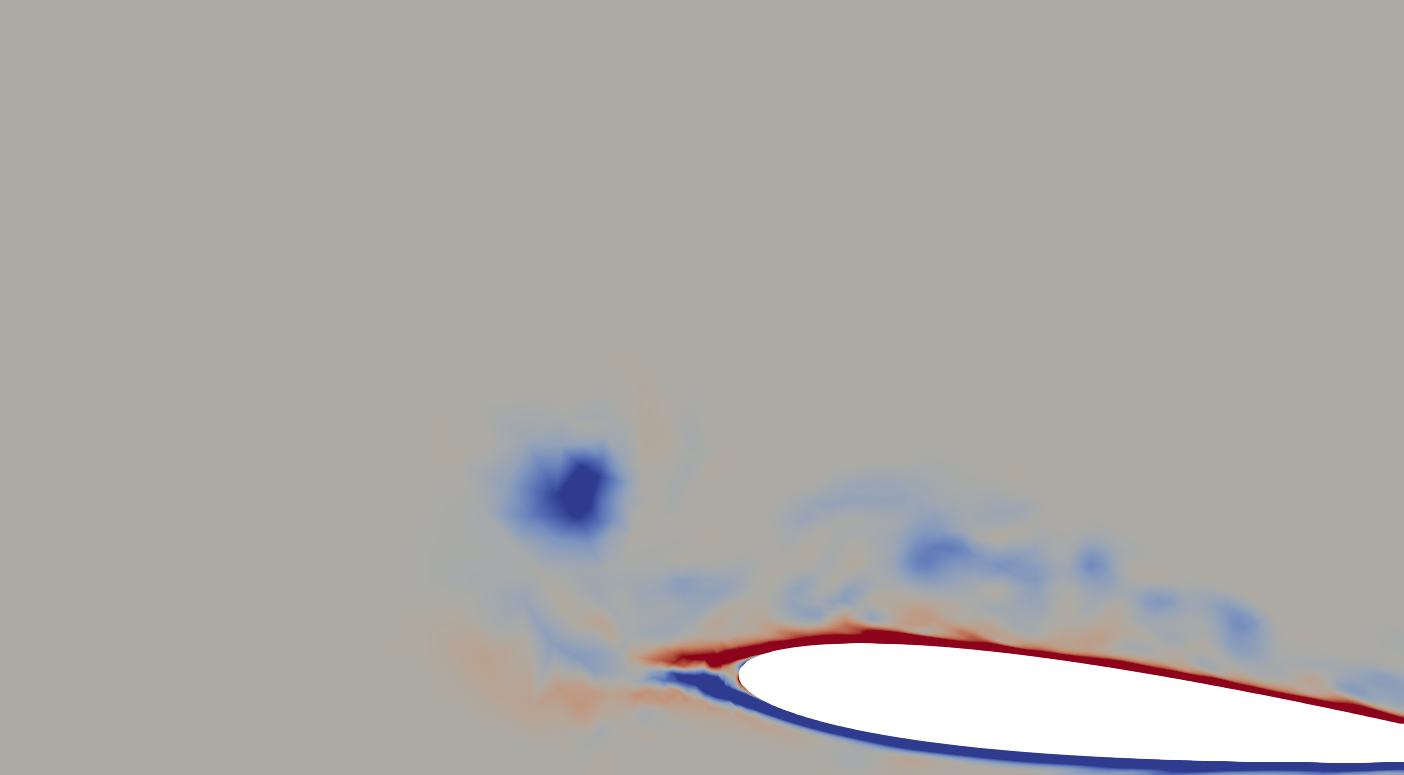
\includegraphics[width=1\textwidth]{figures/zonal_adapt_results/vorticity_plots/v3/M0/spavg/phase_270.png}
		\caption{M0 mesh, $\psi$ = $270^\circ$}
		\label{fig:M0_sp_psi270}
		\end{subfigure}
	\end{center}
	\begin{subfigure}[b]{0.475\textwidth}
	\centering
	
\includegraphics[width=1\textwidth]{figures/zonal_adapt_results/vorticity_plots/v3/Mza1_25/spavg/phase_270.png}
	\caption{Mza1\_25 mesh, $\psi$ = $270^\circ$}
	\label{fig:Mza1_25_sp_psi270}
	\end{subfigure}
	\begin{subfigure}[b]{0.475\textwidth}
		\centering
		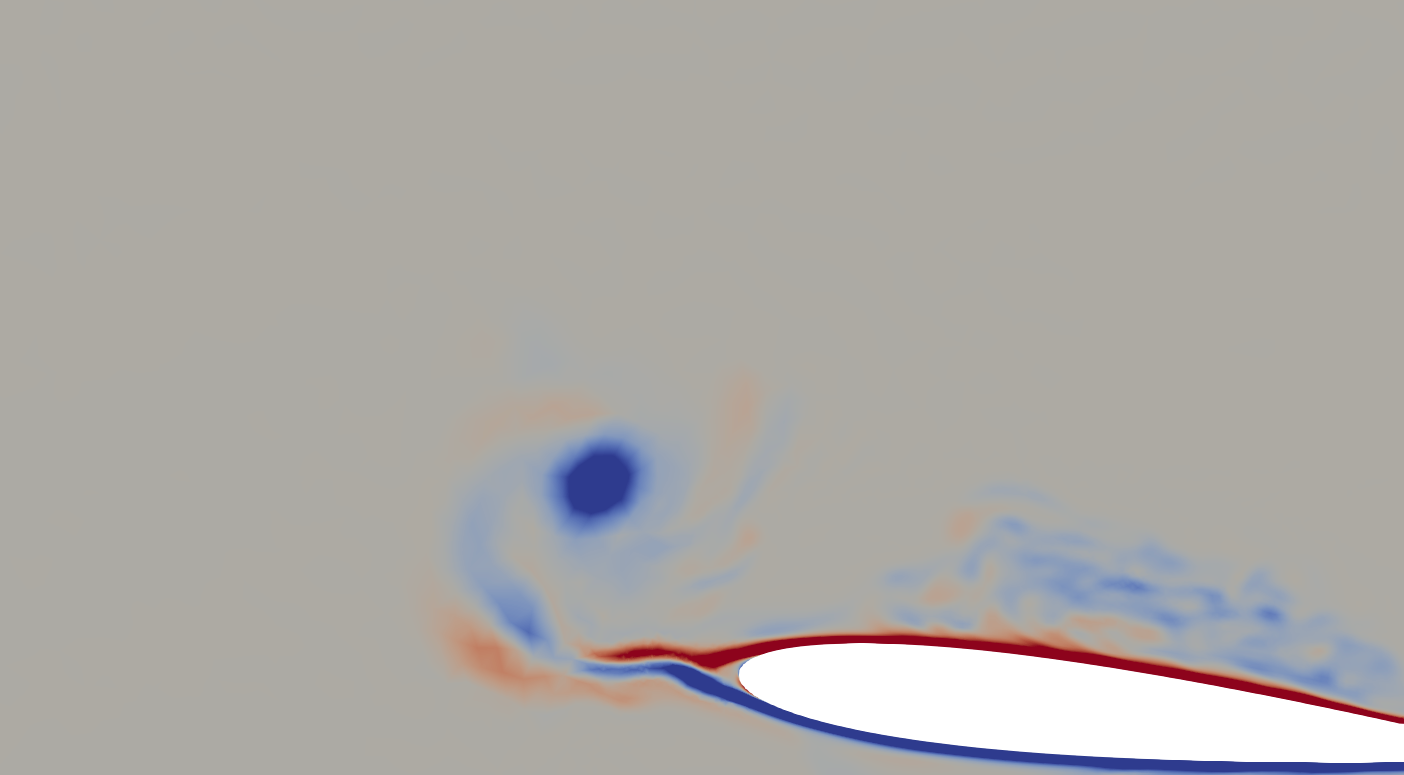
\includegraphics[width=1\textwidth]{figures/zonal_adapt_results/vorticity_plots/v3/Mza1_50/spavg/phase_270.png}
		\caption{Mza1\_50 mesh, $\psi$ = $270^\circ$}
		\label{fig:Mza1_50_sp_psi270}
	\end{subfigure}
%	\begin{subfigure}[b]{0.475\textwidth}
%		\centering
%		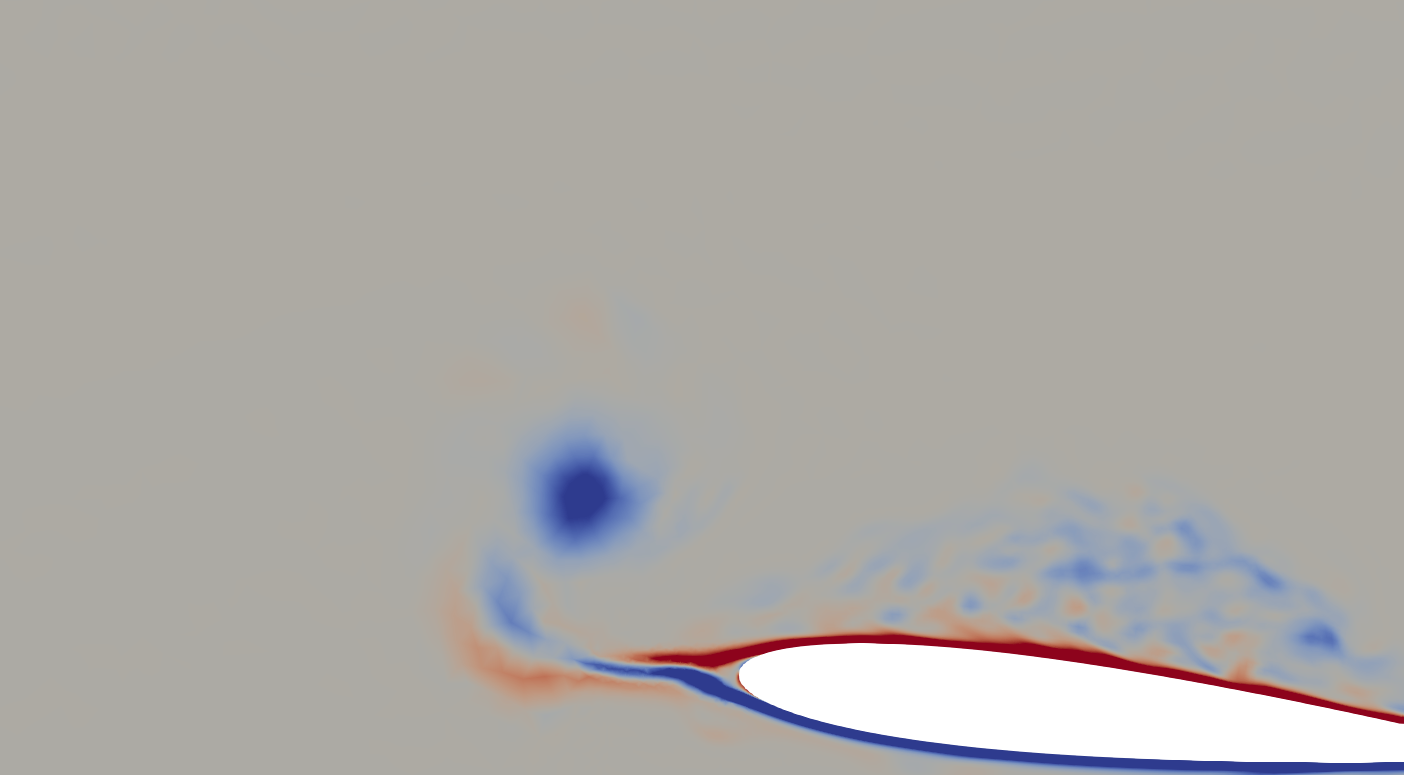
\includegraphics[width=1\textwidth]{figures/zonal_adapt_results/vorticity_plots/v3/Mza1_100/spavg/phase_270.png}
%		\caption{Mza1\_100 mesh, $\psi$ = $270^\circ$}
%		\label{fig:Mza1_100_sp_psi270}
%	\end{subfigure}
%	\begin{subfigure}[b]{0.475\textwidth}
%	\centering
%	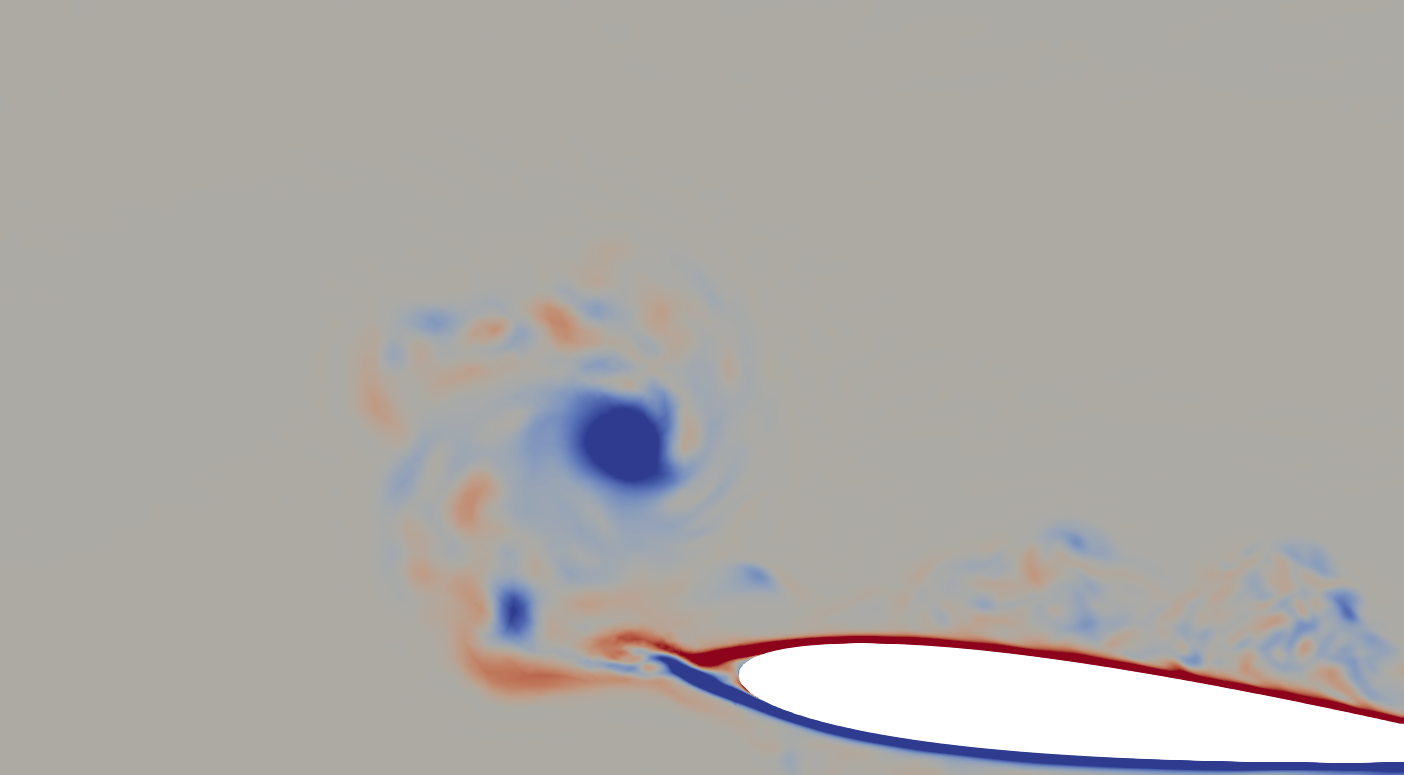
\includegraphics[width=1\textwidth]{figures/zonal_adapt_results/vorticity_plots/v3/Mza2_25/spavg/phase_270.png}
%	\caption{Mza2\_25 mesh, $\psi$ = $270^\circ$}
%	\label{fig:Mza2_25_sp_psi270}
%    \end{subfigure}	
	\begin{subfigure}[b]{0.475\textwidth}
		\centering
		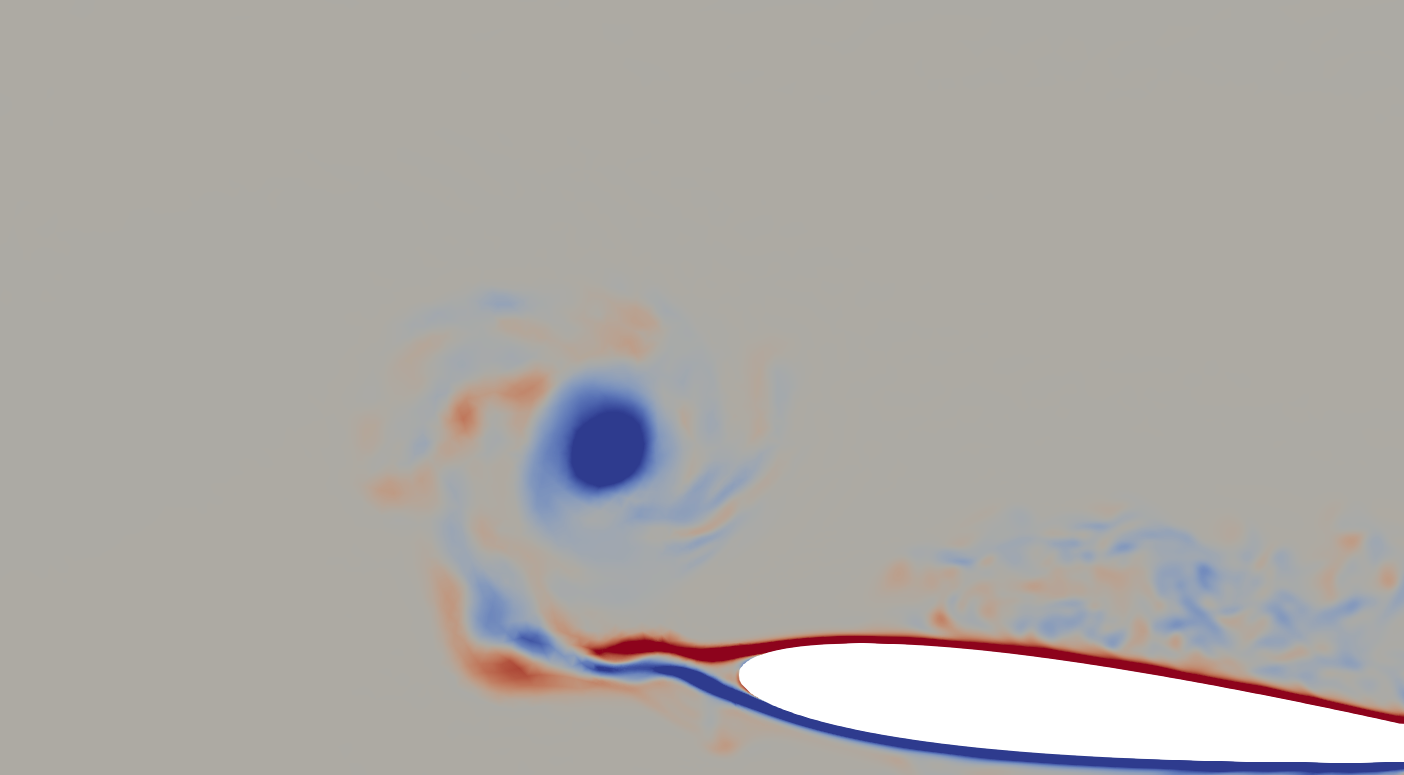
\includegraphics[width=1\textwidth]{figures/zonal_adapt_results/vorticity_plots/v3/Mza2_50/spavg/phase_270.png}
		\caption{Mza2\_50 mesh, $\psi$ = $270^\circ$}
		\label{fig:Mza2_50_sp_psi270}
	\end{subfigure}	
	\begin{subfigure}[b]{0.475\textwidth}
		\centering
		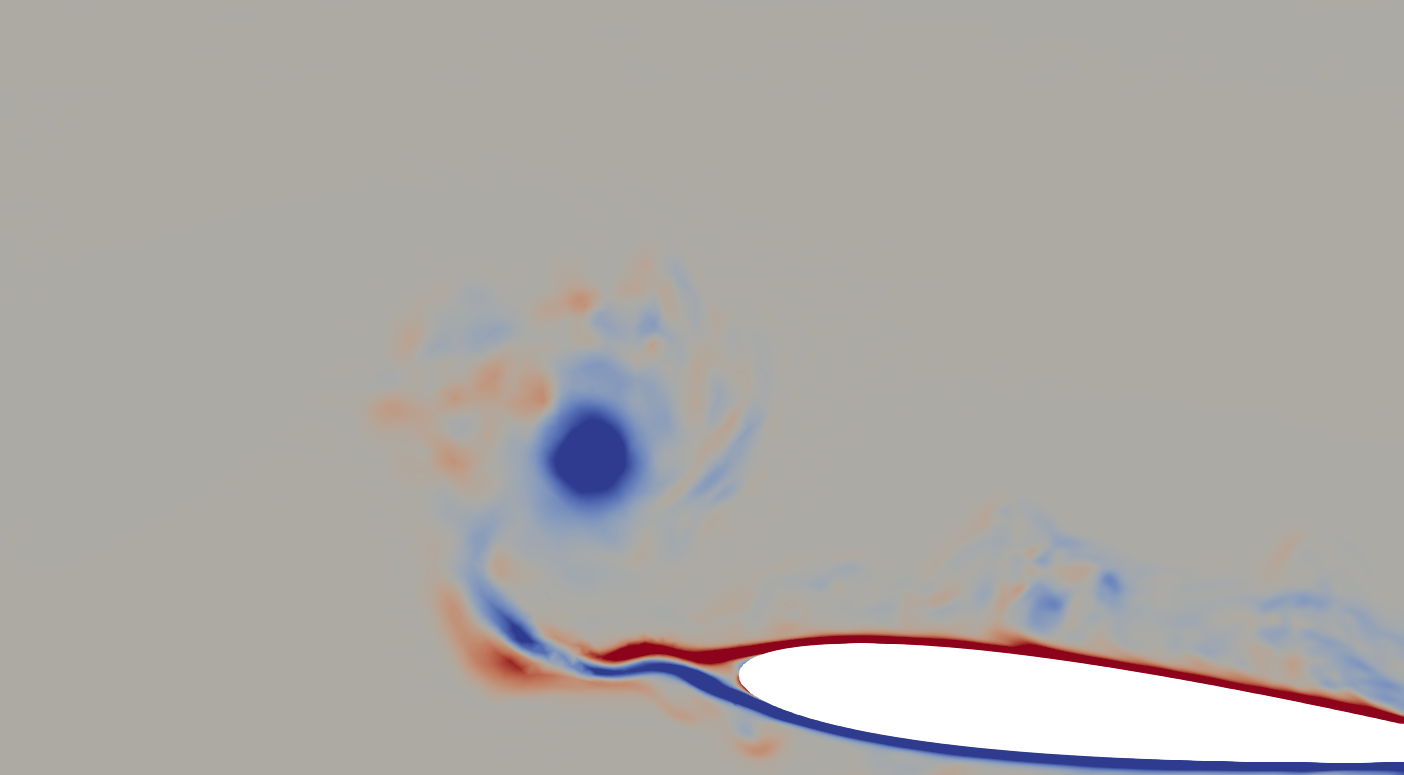
\includegraphics[width=1\textwidth]{figures/zonal_adapt_results/vorticity_plots/v3/Mza2_100/spavg/phase_270.png}
		\caption{Mza2\_100 mesh, $\psi$ = $270^\circ$}
		\label{fig:Mza2_100_sp_psi270}
	\end{subfigure}
	\begin{subfigure}[b]{0.475\textwidth}
	\centering
	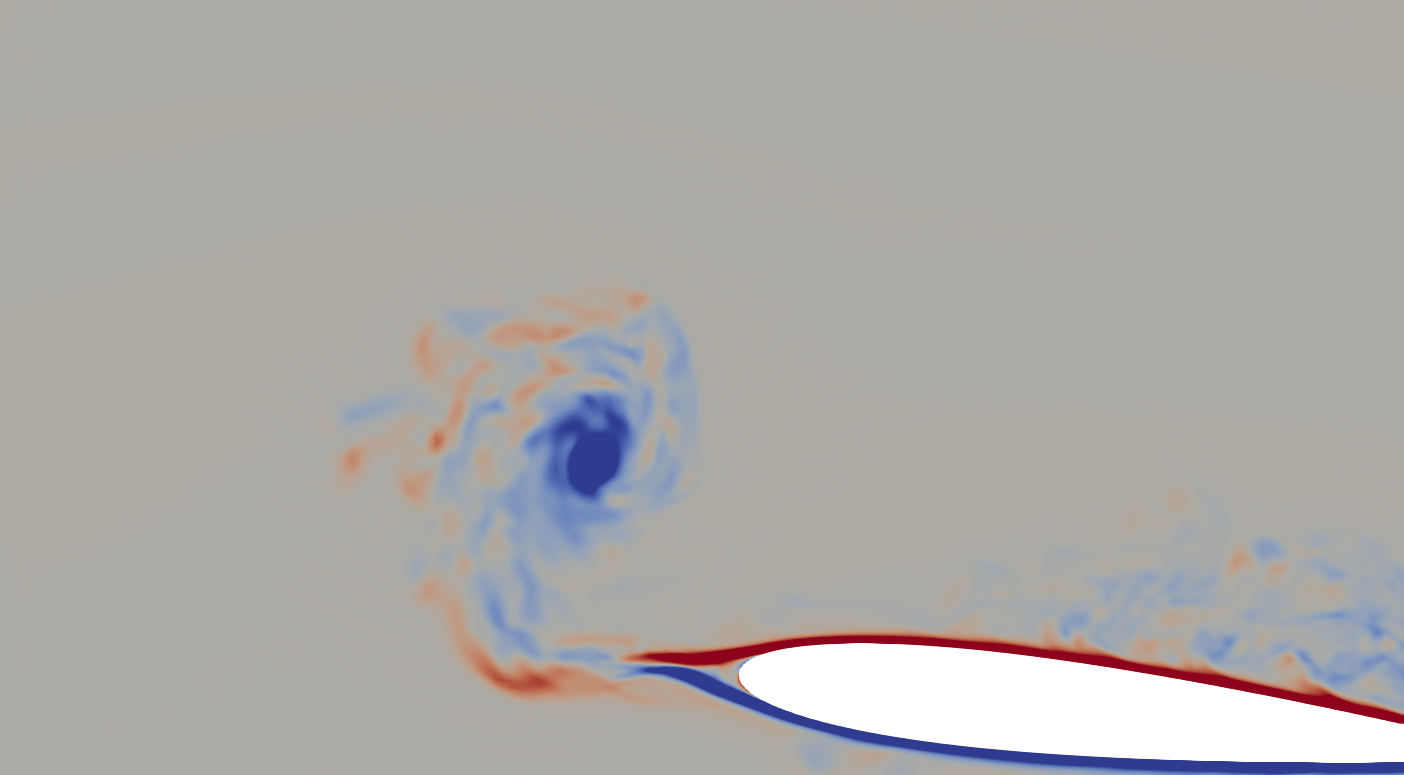
\includegraphics[width=1\textwidth]{figures/zonal_adapt_results/vorticity_plots/v3/Mza3_50/spavg/phase_270.png}
	\caption{Mza3\_50 mesh, $\psi$ = $270^\circ$}
	\label{fig:Mza3_50_sp_psi270}
\end{subfigure}
	\begin{subfigure}[b]{0.475\textwidth}
		\centering
		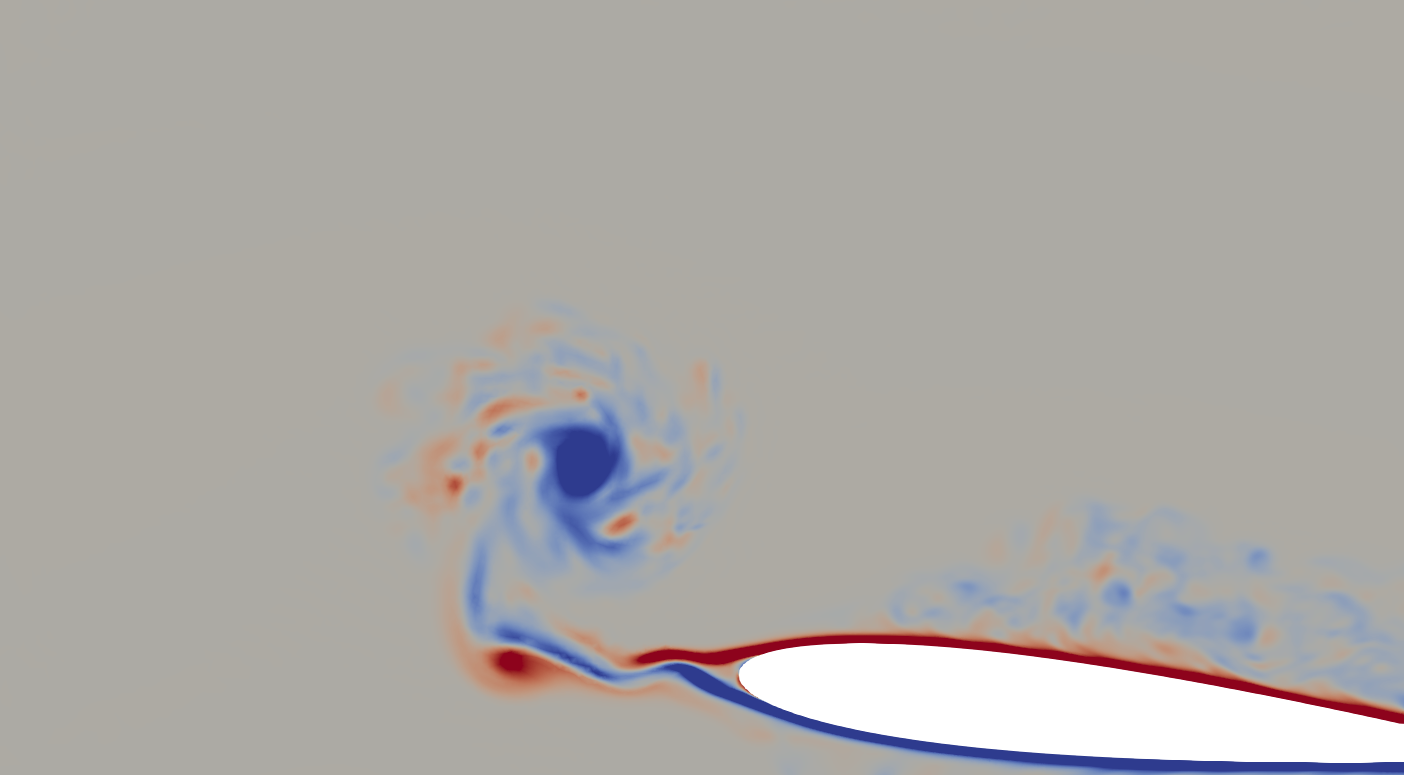
\includegraphics[width=1\textwidth]{figures/zonal_adapt_results/vorticity_plots/v3/Mza3_100/spavg/phase_270.png}
		\caption{Mza3\_100 mesh, $\psi$ = $270^\circ$}
		\label{fig:Mza3_100_sp_psi270}
	\end{subfigure}
	\caption{Spanwise vorticity comparison at $\psi$ = $270^\circ$ for different meshes}
	\label{fig:vorticity_zonal_270}
\end{figure}

\begin{comment}


\begin{figure}[H]
	\centering
	\begin{subfigure}[b]{0.475\textwidth}
		\centering
		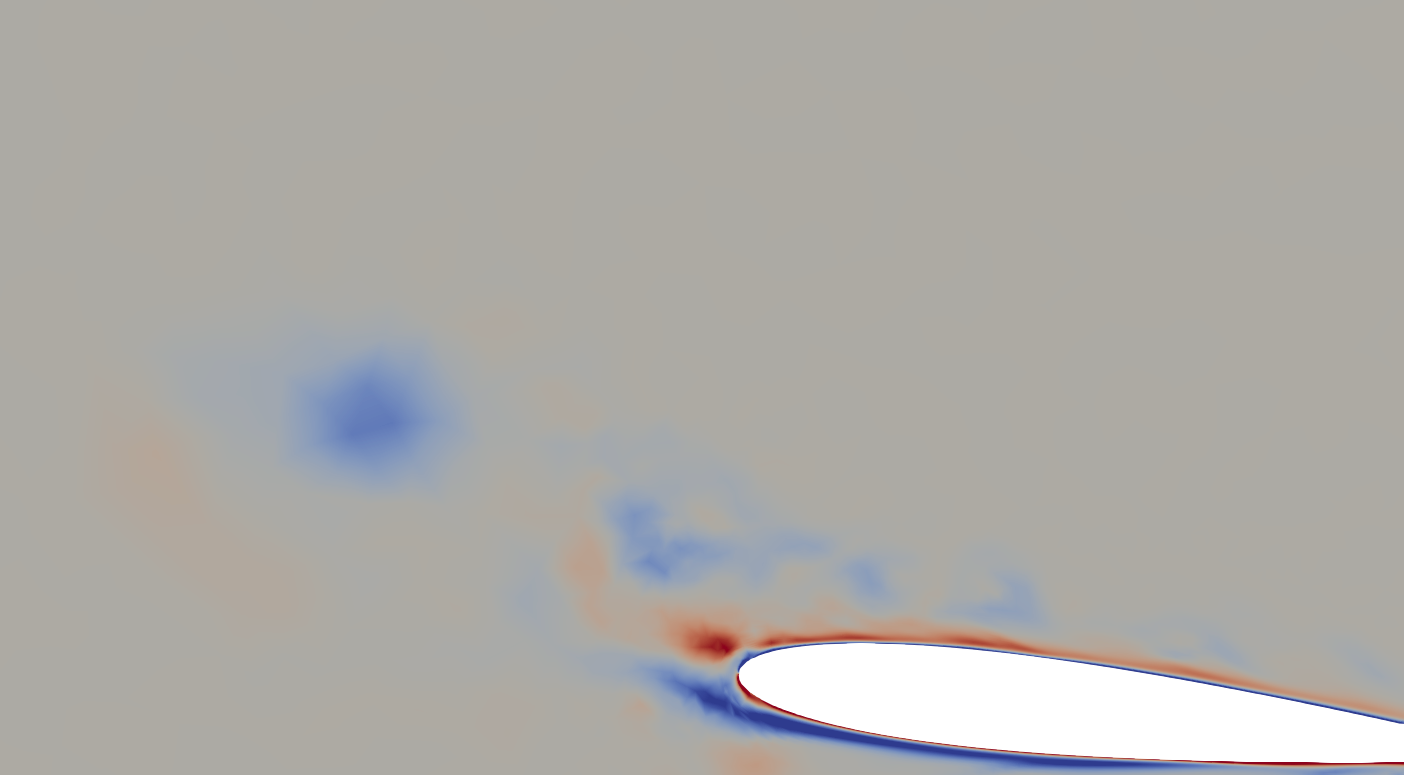
\includegraphics[width=1\textwidth]{figures/zonal_adapt_results/vorticity_plots/v3/M0/spavg/phase_300.png}
		\caption{M0 mesh, $\psi$ = $300^\circ$}
		\label{fig:M0_sp_psi300}
	\end{subfigure}
	\begin{subfigure}[b]{0.475\textwidth}
	\centering
	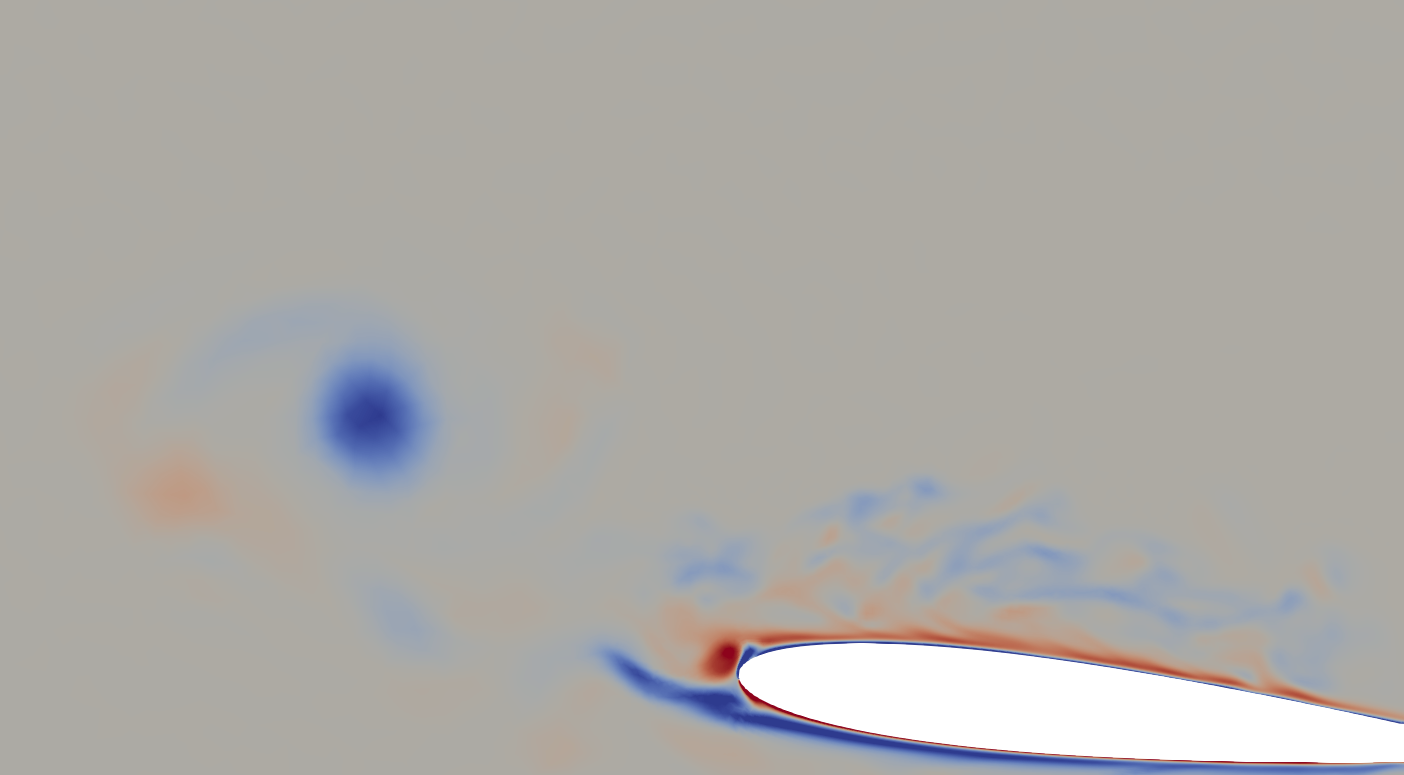
\includegraphics[width=1\textwidth]{figures/zonal_adapt_results/vorticity_plots/v3/Mza1_25/spavg/phase_300.png}
	\caption{Mza1\_25 mesh, $\psi$ = $300^\circ$}
	\label{fig:Mza1_25_sp_psi300}
	\end{subfigure}
	\begin{subfigure}[b]{0.475\textwidth}
		\centering
		\includegraphics[width=1\textwidth]{figures/zonal_adapt_results/vorticity_plots/v3/Mza1_50/spavg/phase_300.png}
		\caption{Mza1\_50 mesh, $\psi$ = $300^\circ$}
		\label{fig:Mza1_50_sp_psi300}
	\end{subfigure}
%	\begin{subfigure}[b]{0.475\textwidth}
%		\centering
%		\includegraphics[width=1\textwidth]{figures/zonal_adapt_results/vorticity_plots/v3/Mza1_100/spavg/phase_300.png}
%		\caption{Mza1\_100 mesh, $\psi$ = $300^\circ$}
%		\label{fig:Mza1_100_sp_psi300}
%	\end{subfigure}
	\begin{subfigure}[b]{0.475\textwidth}
	\centering
	\includegraphics[width=1\textwidth]{figures/zonal_adapt_results/vorticity_plots/v3/Mza2_25/spavg/phase_300.png}
	\caption{Mza2\_25 mesh, $\psi$ = $300^\circ$}
	\label{fig:Mza2_25_sp_psi300}
\end{subfigure}	
	\begin{subfigure}[b]{0.475\textwidth}
		\centering
		\includegraphics[width=1\textwidth]{figures/zonal_adapt_results/vorticity_plots/v3/Mza2_50/spavg/phase_300.png}
		\caption{Mza2\_50 mesh, $\psi$ = $300^\circ$}
		\label{fig:Mza2_50_sp_psi300}
	\end{subfigure}	
	\begin{subfigure}[b]{0.475\textwidth}
		\centering
		\includegraphics[width=1\textwidth]{figures/zonal_adapt_results/vorticity_plots/v3/Mza2_100/spavg/phase_300.png}
		\caption{Mza2\_100 mesh, $\psi$ = $300^\circ$}
		\label{fig:Mza2_100_sp_psi300}
	\end{subfigure}
	\begin{subfigure}[b]{0.475\textwidth}
	\centering
	\includegraphics[width=1\textwidth]{figures/zonal_adapt_results/vorticity_plots/v3/Mza3_50/spavg/phase_300.png}
	\caption{Mza3\_50 mesh, $\psi$ = $300^\circ$}
	\label{fig:Mza3_50_sp_psi300}
\end{subfigure}
	\begin{subfigure}[b]{0.475\textwidth}
		\centering
		\includegraphics[width=1\textwidth]{figures/zonal_adapt_results/vorticity_plots/v3/Mza3_100/spavg/phase_300.png}
		\caption{Mza3\_100 mesh, $\psi$ = $300^\circ$}
		\label{fig:Mza3_100_sp_psi300}
	\end{subfigure}
	\caption{Spanwise vorticity comparison at $\psi$ = $300^\circ$ for different meshes}
	\label{fig:vorticity_zonal_300}
\end{figure}

\end{comment}
=======



In this section, we focus on instantaneous spanwise vorticity for the different meshes considered due to zonal-based refinement/adaptation. Here, instantaneous data is considered since we are interested in observing the flow structures and turbulence captured by different meshes, and obtaining phase-averaged data over multiple cycles can be computationally expensive, especially for the finer meshes, and can also filter out the turbulence in the flow-field.

A comparison of instantaneous spanwise vorticity for the different meshes is shown in Figures \ref{fig:vorticity_zonal_180}, \ref{fig:vorticity_zonal_210}, \ref{fig:vorticity_zonal_240}, and \ref{fig:vorticity_zonal_270} for phases $\psi=180^\circ$, $\psi=210^\circ$, $\psi=240^\circ$, and $\psi=270^\circ$ respectively. For $\psi=180^\circ$, Mza2 and Mza3 meshes show the onset of boundary layer roll-up towards the geometric leading edge over the airfoil surface. M0 and Mza1 meshes fail to capture a significant boundary layer roll-up. Moreover, Mza2 and Mza3 meshes capture more turbulence than M0 and Mza1 meshes, with the flow-structures captured by Mza2 meshes being slightly more diffused than Mza3 meshes. Note that changes in spanwise resolution for the same in-plane mesh do not show any significant variations in the flow-field.

For $\psi=210^\circ$, formation of LEV begins to take place for all meshes apart from M0, as we see a distinct vortex build up near the geometric leading edge, which M0 mesh fails to capture. There is a clear difference between the both the location of the roll-up over the airfoil surface, and the size and extent of the roll-up between Mza1 meshes and Mza2 and Mza3 meshes. The flow-field for Mza2 and Mza3 meshes compare well with each other, with some minor differences due to the flow-field being instantaneous. More fine-scale flow structures are resolved by the finer meshes Mza2 and Mza3, while M0 and Mza1 show poor resolution of these structures.



%%=====================================
%% Phase = 180
%%=====================================


\begin{figure}[H]
	\centering
	\begin{center}
	\begin{subfigure}[b]{0.475\textwidth}
		\centering
		\includegraphics[width=1\textwidth]{figures/zonal_adapt_results/vorticity_plots/v2/M0/spavg/phase_180.png}
		\caption{M0 mesh, $\psi$ = $180^\circ$}
		\label{fig:M0_sp_psi180}
	\end{subfigure}
	\end{center}
	\begin{subfigure}[b]{0.475\textwidth}
	\centering
	\includegraphics[width=1\textwidth]{figures/zonal_adapt_results/vorticity_plots/v2/Mza1_25/spavg/phase_180.png}
	\caption{Mza1\_25 mesh, $\psi$ = $180^\circ$}
	\label{fig:Mza1_25_sp_psi180}
\end{subfigure}
	\begin{subfigure}[b]{0.475\textwidth}
		\centering
		\includegraphics[width=1\textwidth]{figures/zonal_adapt_results/vorticity_plots/v2/Mza1_50/spavg/phase_180.png}
		\caption{Mza1\_50 mesh, $\psi$ = $180^\circ$}
		\label{fig:Mza1_50_sp_psi180}
	\end{subfigure}
%	\begin{subfigure}[b]{0.475\textwidth}
%		\centering
%		\includegraphics[width=1\textwidth]{figures/zonal_adapt_results/vorticity_plots/v2/Mza1_100/spavg/phase_180.png}
%		\caption{Mza1\_100 mesh, $\psi$ = $180^\circ$}
%		\label{fig:Mza1_100_sp_psi180}
%	\end{subfigure}
%	\begin{subfigure}[b]{0.475\textwidth}
%	\centering
%	\includegraphics[width=1\textwidth]{figures/zonal_adapt_results/vorticity_plots/v2/Mza2_25/spavg/phase_180.png}
%	\caption{Mza2\_25 mesh, $\psi$ = $180^\circ$}
%	\label{fig:Mza2_25_sp_psi180}
%	\end{subfigure}
	\begin{subfigure}[b]{0.475\textwidth}
		\centering
		\includegraphics[width=1\textwidth]{figures/zonal_adapt_results/vorticity_plots/v2/Mza2_50/spavg/phase_180.png}
		\caption{Mza2\_50 mesh, $\psi$ = $180^\circ$}
		\label{fig:Mza2_50_sp_psi180}
	\end{subfigure}	
	\begin{subfigure}[b]{0.475\textwidth}
		\centering
		\includegraphics[width=1\textwidth]{figures/zonal_adapt_results/vorticity_plots/v2/Mza2_100/spavg/phase_180.png}
		\caption{Mza2\_100 mesh, $\psi$ = $180^\circ$}
		\label{fig:Mza2_100_sp_psi180}
	\end{subfigure}
	\begin{subfigure}[b]{0.475\textwidth}
	\centering
	\includegraphics[width=1\textwidth]{figures/zonal_adapt_results/vorticity_plots/v2/Mza3_50/spavg/phase_180.png}
	\caption{Mza3\_50 mesh, $\psi$ = $180^\circ$}
	\label{fig:Mza3_100_sp_psi180}
	\end{subfigure}
	\begin{subfigure}[b]{0.475\textwidth}
		\centering
		\includegraphics[width=1\textwidth]{figures/zonal_adapt_results/vorticity_plots/v2/Mza3_100/spavg/phase_180.png}
		\caption{Mza3\_100 mesh, $\psi$ = $180^\circ$}
		\label{fig:Mza3_100_sp_psi180}
	\end{subfigure}
	\caption{Spanwise vorticity comparison at $\psi$ = $180^\circ$ for different meshes}
	\label{fig:vorticity_zonal_180}
\end{figure}

%%=====================================
%% Phase = 210
%%=====================================


\begin{figure}[H]
	\centering
	\begin{center}
		\begin{subfigure}[b]{0.475\textwidth}
		\centering
		\includegraphics[width=1\textwidth]{figures/zonal_adapt_results/vorticity_plots/v2/M0/spavg/phase_210.png}
		\caption{M0 mesh, $\psi$ = $210^\circ$}
		\label{fig:M0_sp_psi210}
		\end{subfigure}
	\end{center}
	\begin{subfigure}[b]{0.475\textwidth}
	\centering
	\includegraphics[width=1\textwidth]{figures/zonal_adapt_results/vorticity_plots/v2/Mza1_25/spavg/phase_210.png}
	\caption{Mza1\_25 mesh, $\psi$ = $210^\circ$}
	\label{fig:Mza1_25_sp_psi210}
	\end{subfigure}
	\begin{subfigure}[b]{0.475\textwidth}
		\centering
		\includegraphics[width=1\textwidth]{figures/zonal_adapt_results/vorticity_plots/v2/Mza1_50/spavg/phase_210.png}
		\caption{Mza1\_50 mesh, $\psi$ = $210^\circ$}
		\label{fig:Mza1_50_sp_psi210}
	\end{subfigure}
%	\begin{subfigure}[b]{0.475\textwidth}
%		\centering
%		\includegraphics[width=1\textwidth]{figures/zonal_adapt_results/vorticity_plots/v2/Mza1_100/spavg/phase_210.png}
%		\caption{Mza1\_100 mesh, $\psi$ = $210^\circ$}
%		\label{fig:Mza1_100_sp_psi210}
%	\end{subfigure}
%	\begin{subfigure}[b]{0.475\textwidth}
%	\centering
%	\includegraphics[width=1\textwidth]{figures/zonal_adapt_results/vorticity_plots/v2/Mza2_25/spavg/phase_210.png}
%	\caption{Mza2\_25 mesh, $\psi$ = $210^\circ$}
%	\label{fig:Mza2_25_sp_psi210}
%	\end{subfigure}	
	\begin{subfigure}[b]{0.475\textwidth}
		\centering
		\includegraphics[width=1\textwidth]{figures/zonal_adapt_results/vorticity_plots/v2/Mza2_50/spavg/phase_210.png}
		\caption{Mza2\_50 mesh, $\psi$ = $210^\circ$}
		\label{fig:Mza2_50_sp_psi210}
	\end{subfigure}	
	\begin{subfigure}[b]{0.475\textwidth}
		\centering
		\includegraphics[width=1\textwidth]{figures/zonal_adapt_results/vorticity_plots/v2/Mza2_100/spavg/phase_210.png}
		\caption{Mza2\_100 mesh, $\psi$ = $210^\circ$}
		\label{fig:Mza2_100_sp_psi210}
	\end{subfigure}
	\begin{subfigure}[b]{0.475\textwidth}
	\centering
	\includegraphics[width=1\textwidth]{figures/zonal_adapt_results/vorticity_plots/v2/Mza3_50/spavg/phase_210.png}
	\caption{Mza3\_50 mesh, $\psi$ = $210^\circ$}
	\label{fig:Mza3_50_sp_psi210}
\end{subfigure}
	\begin{subfigure}[b]{0.475\textwidth}
		\centering
		\includegraphics[width=1\textwidth]{figures/zonal_adapt_results/vorticity_plots/v2/Mza3_100/spavg/phase_210.png}
		\caption{Mza3\_100 mesh, $\psi$ = $210^\circ$}
		\label{fig:Mza3_100_sp_psi210}
	\end{subfigure}
	\caption{Spanwise vorticity comparison at $\psi$ = $210^\circ$ for different meshes}
	\label{fig:vorticity_zonal_210}
\end{figure}

%%=====================================
%% Phase = 240
%%=====================================


\begin{figure}[H]
	\centering
	\begin{center}
		\begin{subfigure}[b]{0.475\textwidth}
		\centering
		\includegraphics[width=1\textwidth]{figures/zonal_adapt_results/vorticity_plots/v2/M0/spavg/phase_240.png}
		\caption{M0 mesh, $\psi$ = $240^\circ$}
		\label{fig:M0_sp_psi240}
		\end{subfigure}
	\end{center}
	\begin{subfigure}[b]{0.475\textwidth}
		\centering
		\includegraphics[width=1\textwidth]{figures/zonal_adapt_results/vorticity_plots/v2/Mza1_25/spavg/phase_240.png}
		\caption{Mza1\_25 mesh, $\psi$ = $240^\circ$}
		\label{fig:Mza1_25_sp_psi240}
	\end{subfigure}
	\begin{subfigure}[b]{0.475\textwidth}
	\centering
	\includegraphics[width=1\textwidth]{figures/zonal_adapt_results/vorticity_plots/v2/Mza1_50/spavg/phase_240.png}
	\caption{Mza1\_50 mesh, $\psi$ = $240^\circ$}
	\label{fig:Mza1_50_sp_psi240}
	\end{subfigure}
	\begin{subfigure}[b]{0.475\textwidth}
		\centering
		\includegraphics[width=1\textwidth]{figures/zonal_adapt_results/vorticity_plots/v2/Mza2_50/spavg/phase_240.png}
		\caption{Mza2\_50 mesh, $\psi$ = $240^\circ$}
		\label{fig:Mza2_50_sp_psi240}
	\end{subfigure}
%	\begin{subfigure}[b]{0.475\textwidth}
%		\centering
%		\includegraphics[width=1\textwidth]{figures/zonal_adapt_results/vorticity_plots/v2/Mza1_100/spavg/phase_240.png}
%		\caption{Mza1\_100 mesh, $\psi$ = $240^\circ$}
%		\label{fig:Mza1_100_sp_psi240}
%	\end{subfigure}
%	\begin{subfigure}[b]{0.475\textwidth}
%	\centering
%	\includegraphics[width=1\textwidth]{figures/zonal_adapt_results/vorticity_plots/v2/Mza2_25/spavg/phase_240.png}
%	\caption{Mza2\_25 mesh, $\psi$ = $240^\circ$}
%	\label{fig:Mza2_25_sp_psi240}
%	\end{subfigure}	
%	\begin{subfigure}[b]{0.475\textwidth}
%		\centering
%		\includegraphics[width=1\textwidth]{figures/zonal_adapt_results/vorticity_plots/v2/Mza2_50/spavg/phase_240.png}
%		\caption{Mza2\_50 mesh, $\psi$ = $240^\circ$}
%		\label{fig:Mza2_50_sp_psi240}
%	\end{subfigure}	
	\begin{subfigure}[b]{0.475\textwidth}
		\centering
		\includegraphics[width=1\textwidth]{figures/zonal_adapt_results/vorticity_plots/v2/Mza2_100/spavg/phase_240.png}
		\caption{Mza2\_100 mesh, $\psi$ = $240^\circ$}
		\label{fig:Mza2_100_sp_psi240}
	\end{subfigure}
	\begin{subfigure}[b]{0.475\textwidth}
	\centering
	\includegraphics[width=1\textwidth]{figures/zonal_adapt_results/vorticity_plots/v2/Mza3_50/spavg/phase_240.png}
	\caption{Mza3\_50 mesh, $\psi$ = $240^\circ$}
	\label{fig:Mza3_100_sp_psi240}
\end{subfigure}
	\begin{subfigure}[b]{0.475\textwidth}
		\centering
		\includegraphics[width=1\textwidth]{figures/zonal_adapt_results/vorticity_plots/v2/Mza3_100/spavg/phase_240.png}
		\caption{Mza3\_100 mesh, $\psi$ = $240^\circ$}
		\label{fig:Mza3_100_sp_psi240}
	\end{subfigure}
	\caption{Spanwise vorticity comparison at $\psi$ = $240^\circ$ for different meshes}
	\label{fig:vorticity_zonal_240}
\end{figure}

%%=====================================
%% Phase = 270
%%=====================================


\begin{figure}[H]
	\centering
	\begin{center}
		\begin{subfigure}[b]{0.475\textwidth}
		\centering
		\includegraphics[width=1\textwidth]{figures/zonal_adapt_results/vorticity_plots/v3/M0/spavg/phase_270.png}
		\caption{M0 mesh, $\psi$ = $270^\circ$}
		\label{fig:M0_sp_psi270}
		\end{subfigure}
	\end{center}
	\begin{subfigure}[b]{0.475\textwidth}
	\centering
	\includegraphics[width=1\textwidth]{figures/zonal_adapt_results/vorticity_plots/v3/Mza1_25/spavg/phase_270.png}
	\caption{Mza1\_25 mesh, $\psi$ = $270^\circ$}
	\label{fig:Mza1_25_sp_psi270}
	\end{subfigure}
	\begin{subfigure}[b]{0.475\textwidth}
		\centering
		\includegraphics[width=1\textwidth]{figures/zonal_adapt_results/vorticity_plots/v3/Mza1_50/spavg/phase_270.png}
		\caption{Mza1\_50 mesh, $\psi$ = $270^\circ$}
		\label{fig:Mza1_50_sp_psi270}
	\end{subfigure}
%	\begin{subfigure}[b]{0.475\textwidth}
%		\centering
%		\includegraphics[width=1\textwidth]{figures/zonal_adapt_results/vorticity_plots/v3/Mza1_100/spavg/phase_270.png}
%		\caption{Mza1\_100 mesh, $\psi$ = $270^\circ$}
%		\label{fig:Mza1_100_sp_psi270}
%	\end{subfigure}
%	\begin{subfigure}[b]{0.475\textwidth}
%	\centering
%	\includegraphics[width=1\textwidth]{figures/zonal_adapt_results/vorticity_plots/v3/Mza2_25/spavg/phase_270.png}
%	\caption{Mza2\_25 mesh, $\psi$ = $270^\circ$}
%	\label{fig:Mza2_25_sp_psi270}
%    \end{subfigure}	
	\begin{subfigure}[b]{0.475\textwidth}
		\centering
		\includegraphics[width=1\textwidth]{figures/zonal_adapt_results/vorticity_plots/v3/Mza2_50/spavg/phase_270.png}
		\caption{Mza2\_50 mesh, $\psi$ = $270^\circ$}
		\label{fig:Mza2_50_sp_psi270}
	\end{subfigure}	
	\begin{subfigure}[b]{0.475\textwidth}
		\centering
		\includegraphics[width=1\textwidth]{figures/zonal_adapt_results/vorticity_plots/v3/Mza2_100/spavg/phase_270.png}
		\caption{Mza2\_100 mesh, $\psi$ = $270^\circ$}
		\label{fig:Mza2_100_sp_psi270}
	\end{subfigure}
	\begin{subfigure}[b]{0.475\textwidth}
	\centering
	\includegraphics[width=1\textwidth]{figures/zonal_adapt_results/vorticity_plots/v3/Mza3_50/spavg/phase_270.png}
	\caption{Mza3\_50 mesh, $\psi$ = $270^\circ$}
	\label{fig:Mza3_50_sp_psi270}
\end{subfigure}
	\begin{subfigure}[b]{0.475\textwidth}
		\centering
		\includegraphics[width=1\textwidth]{figures/zonal_adapt_results/vorticity_plots/v3/Mza3_100/spavg/phase_270.png}
		\caption{Mza3\_100 mesh, $\psi$ = $270^\circ$}
		\label{fig:Mza3_100_sp_psi270}
	\end{subfigure}
	\caption{Spanwise vorticity comparison at $\psi$ = $270^\circ$ for different meshes}
	\label{fig:vorticity_zonal_270}
\end{figure}

\begin{comment}


\begin{figure}[H]
	\centering
	\begin{subfigure}[b]{0.475\textwidth}
		\centering
		\includegraphics[width=1\textwidth]{figures/zonal_adapt_results/vorticity_plots/v3/M0/spavg/phase_300.png}
		\caption{M0 mesh, $\psi$ = $300^\circ$}
		\label{fig:M0_sp_psi300}
	\end{subfigure}
	\begin{subfigure}[b]{0.475\textwidth}
	\centering
	\includegraphics[width=1\textwidth]{figures/zonal_adapt_results/vorticity_plots/v3/Mza1_25/spavg/phase_300.png}
	\caption{Mza1\_25 mesh, $\psi$ = $300^\circ$}
	\label{fig:Mza1_25_sp_psi300}
	\end{subfigure}
	\begin{subfigure}[b]{0.475\textwidth}
		\centering
		\includegraphics[width=1\textwidth]{figures/zonal_adapt_results/vorticity_plots/v3/Mza1_50/spavg/phase_300.png}
		\caption{Mza1\_50 mesh, $\psi$ = $300^\circ$}
		\label{fig:Mza1_50_sp_psi300}
	\end{subfigure}
%	\begin{subfigure}[b]{0.475\textwidth}
%		\centering
%		\includegraphics[width=1\textwidth]{figures/zonal_adapt_results/vorticity_plots/v3/Mza1_100/spavg/phase_300.png}
%		\caption{Mza1\_100 mesh, $\psi$ = $300^\circ$}
%		\label{fig:Mza1_100_sp_psi300}
%	\end{subfigure}
	\begin{subfigure}[b]{0.475\textwidth}
	\centering
	\includegraphics[width=1\textwidth]{figures/zonal_adapt_results/vorticity_plots/v3/Mza2_25/spavg/phase_300.png}
	\caption{Mza2\_25 mesh, $\psi$ = $300^\circ$}
	\label{fig:Mza2_25_sp_psi300}
\end{subfigure}	
	\begin{subfigure}[b]{0.475\textwidth}
		\centering
		\includegraphics[width=1\textwidth]{figures/zonal_adapt_results/vorticity_plots/v3/Mza2_50/spavg/phase_300.png}
		\caption{Mza2\_50 mesh, $\psi$ = $300^\circ$}
		\label{fig:Mza2_50_sp_psi300}
	\end{subfigure}	
	\begin{subfigure}[b]{0.475\textwidth}
		\centering
		\includegraphics[width=1\textwidth]{figures/zonal_adapt_results/vorticity_plots/v3/Mza2_100/spavg/phase_300.png}
		\caption{Mza2\_100 mesh, $\psi$ = $300^\circ$}
		\label{fig:Mza2_100_sp_psi300}
	\end{subfigure}
	\begin{subfigure}[b]{0.475\textwidth}
	\centering
	\includegraphics[width=1\textwidth]{figures/zonal_adapt_results/vorticity_plots/v3/Mza3_50/spavg/phase_300.png}
	\caption{Mza3\_50 mesh, $\psi$ = $300^\circ$}
	\label{fig:Mza3_50_sp_psi300}
\end{subfigure}
	\begin{subfigure}[b]{0.475\textwidth}
		\centering
		\includegraphics[width=1\textwidth]{figures/zonal_adapt_results/vorticity_plots/v3/Mza3_100/spavg/phase_300.png}
		\caption{Mza3\_100 mesh, $\psi$ = $300^\circ$}
		\label{fig:Mza3_100_sp_psi300}
	\end{subfigure}
	\caption{Spanwise vorticity comparison at $\psi$ = $300^\circ$ for different meshes}
	\label{fig:vorticity_zonal_300}
\end{figure}

\end{comment}
>>>>>>> d33a82ce4ca8ceb0b9a6b6f66cff859f14e4b38b

\label{sec:zonal_vorticity}

\section{Cp}
%%Cp plots

In this section, we focus on $C_p$ for the different meshes considered due to zonal-based refinement/adaptation. Here, phase averaged and spanwise averaged data is considered over multiple cycles.

A comparison of $C_p$ for the different meshes is shown in Figure \ref{fig:zonal_Cp_plots_LEV}, for four phases of interest leading up to the LEV formation. For phase $\psi=150^\circ$, flow has started to separate for Mza2 and Mza3 meshes around $x/c = 0.2$, whereas M0 and Mza1 meshes fail to capture this flow separation. These differences in separation/boundary layer roll-up can also be seen in the spanwise vorticity plots in Figures \ref{fig:vorticity_zonal_150}.

For phase $\psi=180^\circ$, Mza1 meshes also show boundary layer/vorticity roll-up with a peak in $C_p$ around $x/c = 0.1$. This peak, however, does not match with the peak in $C_p$ in Mza2 and Mza3 meshes, and is also not clearly visible in spanwise vorticity plots shown in Figure \ref{fig:vorticity_zonal_180}. M0 mesh fails to capture this peak in $C_p$. 


For phase $\psi=210^\circ$, all meshes show LEV formation apart from M0 mesh. Note that the peak in $C_p$ corresponds with the low pressure region of the LEV core. Note that the peak and the drop in $C_p$ occurs between $x/c=0.15$ and $x/c=0.22$ for Mza1 meshes. For Mza2 and Mza3 meshes, this event occurs between $x/c=0.25$ and $x/c=0.35$.

For phase $\psi=240^\circ$, LEV formation can be seen for all the meshes, however peak in $C_p$ differs between different meshes. M0 mesh predicts a peak around $x/c=0.1$, whereas Mza1 meshes predict a peak and drop in $C_p$ around $x/c=0.13$ and $x/c=0.22$. Mza2 and Mza3 meshes predict a peak in $C_p$ around $x/c=0.17$ and $x/c=0.3$. Once again, it is observed that Mza2 and Mza3 meshes show reasonable agreement. Also, meshes with same in-plane resolution considered here do not show significant variations with changes in spanwise resolution.




\subsection{Cp: LEV}
\begin{figure}[H]
\centering

\begin{subfigure}[b]{0.475\textwidth}
	\centering
	\includegraphics[width=1\textwidth]{figures/zonal_adapt_results/Cp/phase_150.png}
	\caption{ $C_p$ at $\psi$ = $150^\circ$}
	\label{fig:zonal_Cp_150}
\end{subfigure}
\begin{subfigure}[b]{0.475\textwidth}
\centering
\includegraphics[width=1\textwidth]{figures/zonal_adapt_results/Cp/phase_180.png}
\caption{ $C_p$ at $\psi$ = $180^\circ$}
\label{fig:zonal_Cp_180}
\end{subfigure}
\begin{subfigure}[b]{0.475\textwidth}
\centering
\includegraphics[width=1\textwidth]{figures/zonal_adapt_results/Cp/phase_210.png}
\caption{ $C_p$ at $\psi$ = $210^\circ$}
\label{fig:zonal_Cp_210}
\end{subfigure}
\begin{subfigure}[b]{0.475\textwidth}
\centering
\includegraphics[width=1\textwidth]{figures/zonal_adapt_results/Cp/phase_240.png}
\caption{ $C_p$ at $\psi$ = $240^\circ$}
\label{fig:zonal_Cp_240}
\end{subfigure}
\caption{$C_p$ comparison for different meshes. Top surface $C_p$ is denoted by solid lines and bottom surface $C_p$ is denoted by dashed lines}
\label{fig:zonal_Cp_plots_LEV}
\end{figure}


\subsection{Cp: Trailing Edge Separation}


Since we have already seen through spanwise vorticity plots and Cp that the spanwise resolution of the meshes considered does not affect the solution significantly [need to figure out a better way to say this], we only show data from meshes with the 2nd highest spanwise resolution for brevity. $C_p$ for phases $\psi=270^\circ$ and $\psi=300^\circ$ which is shown in Figure \ref{fig:zonal_Cp_plots_TEV} show formation of trailing edge separation, which is evident from peaks in $C_p$ near the geometric trailing edge. For both these phases, all meshes compare well with each other apart from M0 mesh.


\begin{figure}
\begin{subfigure}[b]{0.475\textwidth}
\centering
\includegraphics[width=1\textwidth]{figures/zonal_adapt_results/Cp/phase_270.png}
\caption{ $C_p$ at $\psi$ = $270^\circ$}
\label{fig:zonal_Cp_270}
\end{subfigure}
\begin{subfigure}[b]{0.475\textwidth}
\centering
\includegraphics[width=1\textwidth]{figures/zonal_adapt_results/Cp/phase_300.png}
\caption{ $C_p$ at $\psi$ = $300^\circ$}
\label{fig:zonal_Cp_300}
\end{subfigure}
\caption{$C_p$ comparison for different meshes. Top surface $C_p$ is denoted by solid lines and bottom surface $C_p$ is denoted by dashed lines}
\label{fig:zonal_Cp_plots_TEV}
\end{figure}


\label{sec:zonal_cp}

\section{LEV}
Using the LEV tracking and quantification algorithm mentioned in chapter \ref{sec:LEV}, a quantitative comparison of the LEV is presented in this section. 
Recall that only results from meshes with the 2nd highest spanwise resolution are considered here for brevity, since it was previously established that results between highest and second highest spanwise resolutions compare well with each other. 
Also note that that phase-averaged and spanwise averaged data over multiple cycles is used here.

Figure \ref{fig:zonal_LEV_location} shows the location of the center of the LEV core for different phases after it is ejected from the airfoil surface. 
It is observed that LEV formation for M0 mesh occurs closer to the geometric leading edge, as well as closer to the airfoil surface as compared to the other meshes.
For the initial phase of LEV location, Mza2 and Mza3 shows differences, where Mza3 mesh shows LEV formation closer to the airfoil surface and also closer to the geometric leading edge as compared to Mza2 mesh.
LEV paths converge as the mesh resolution in the later phases, with Mza2 and Mza3 meshes showing a similar LEV path.


\begin{figure}[H]
	\centering
	\includegraphics[width=0.75\textwidth]{figures/zonal_adapt_results/LEV/LEV_location}
	\caption{ LEV location for different meshes}
	\label{fig:zonal_LEV_location}
\end{figure}

Figure \ref{fig:zonal_utheta_LEV} shows the tangential velocity profiles for the LEV core for different meshes at phases  $\psi = 240^\circ$,  $\psi = 270^\circ$, and  $\psi = 300^\circ$. 
Note that tangential velocity is computed along multiple radial lines passing through the LEV center, and the mean tangential velocity over these radial lines is shown in \ref{fig:zonal_utheta_LEV}, along with a 95\% confidence interval around the mean.
The radial distance from the center of the LEV, $r$, is normalized by the peak radius of the LEV core $r_p$ of the finest mesh Mza3 at that particular phase. 
Here, the peak radius is the radius/location at which maximum tangential velocity is achieved. 
Note that the maximum of the mean of the tangential velocity across multiple radial lines is used here. 

For $\psi = 240^\circ$, max $u_\theta$ is achieved around $r/r_p= 0.6$ for M0 mesh and around $r/r_p= 0.8$ for Mza1 mesh, indicating that a smaller LEV core is predicted for M0 and Mza1 meshes as compared to the finer meshes. 
For Mza2 and Mza3 meshes, the max $u_\theta$ is achieved at $r/r_p = 1$. Note that since $r$ is normalized with $r_p$ for Mza3 mesh, max $r/r_p$ will always be 1 for Mza3 mesh. 
Mean tangential velocity profile for both Mza2 and Mza3 meshes, along with the 95\% confidence interval agree with each other. 
Also note that the large thickness of the confidence interval band around the mean, which can be attributed to the LEV core being azimuthally asymmetric, since the LEV in this phase is close to the airfoil surface, as can be seen in Figure \ref{fig:vorticity_zonal_240}. 

For $\psi = 270^\circ$, max $u_\theta$ is achieved around $r/r_p= 1$ for all meshes. 
M0 and Mza1 meshes predict a lower tangential velocity as compared fto Mza2 and Mza3 meshes. 
Mean tangential velocity profile for Mza2 and Mza3 meshes agree well with each other, with Mza2 mesh predicting slightly higher tangential velocity than Mza3 mesh. 
The confidence interval for Mza3 mesh lies within the confidence interval for Mza2 mesh.

At $\psi = 300^\circ$, for Mza2 and Mza3, both the mean and confidence interval for the tangential velocity matches very well, apart for slight differences at higher $r/r_p$ values. 
Peak $u_\theta$ for both these meshes is around $r/r_p= 1$.
Also note that the thickness/width of the confidence interval has reduced significantly as compared to the previous phases, showing that the LEV core is more azimuthally symmetric at this phase than the previous phases, as it is further away from the airfoil surface.
Mza1 predicts a lower tangential velocity than the finer meshes, with peak $u_\theta$ around $r/r_p= 1.2$. M0 mesh predicts the lowest tangential velocity, and the peak $u_\theta$ is not reached within $r/r_p= 1.25$.

\begin{figure}[H]
	\centering
	\begin{subfigure}[b]{0.475\textwidth}
	\centering
	\includegraphics[width=1\textwidth]{figures/zonal_adapt_results/LEV/u_theta/phase_240.png}
	\caption{ $u_\theta$ at $\psi$ = $240^\circ$}
	\label{fig:zonal_utheta_240}
	\end{subfigure}
	\begin{subfigure}[b]{0.475\textwidth}
	\centering
	\includegraphics[width=1\textwidth]{figures/zonal_adapt_results/LEV/u_theta/phase_270.png}
	\caption{ $u_\theta$ at $\psi$ = $270^\circ$}
	\label{fig:zonal_utheta_270}
    \end{subfigure}
	\begin{subfigure}[b]{0.475\textwidth}
	\centering
	\includegraphics[width=1\textwidth]{figures/zonal_adapt_results/LEV/u_theta/phase_300.png}
	\caption{ $u_\theta$ at $\psi$ = $300^\circ$}
	\label{fig:zonal_utheta_300}
	\end{subfigure}
    \label{fig:zonal_utheta_LEV}
   	\caption{Tangential velocity profiles of LEV at different phases with 95\% confidence interval}
\end{figure}


Figure \ref{fig:zonal_LEV_radius} shows the radius of the LEV. Note that LEV radius is considered at where maximum tangential velocity is achieved.
Recall that tangential velocity is computed along multiple radial lines, and the peak tangential velocity is obtained from this averaged tangential velocity along multiple radial lines. 
In the initial phases when LEV is close to the airfoil surface, Mza2 and Mza3 meshes predict a larger LEV radius than the coarser meshes. 
This difference in size can also be seen in the spanwise vorticity plots shown in Figure \ref{fig:vorticity_zonal_240}.
From phase $\psi = 270^\circ$ and onwards when the LEV is away from the airfoil surface, Mza3 which is the finest mesh, predicts the smallest LEV radius, followed by the second finest mesh, Mza2. 
This is expected, since a finer mesh will have a less diffused vortex core. Also note that M0 mesh completely fails to predict the trend in LEV radius that Mza1, Mza2, and Mza3 meshes show.

\begin{figure}[H]
	\centering
	\includegraphics[width=0.7\textwidth]{figures/zonal_adapt_results/LEV/LEV_radius_vp}
	\caption{ LEV radius for different meshes}
	\label{fig:zonal_LEV_radius}
\end{figure}

Figure \ref{fig:zonal_TI_plots_LEV} shows mean turbulence intensity for LEV for phases $\psi = 240^\circ$, $\psi = 270^\circ$, and $\psi = 300^\circ$. 
Note that mean is taken along multiple radial lines passing through center of LEV core, in a similar fashion to tangential velocity profiles.

At phase $\psi = 240^\circ$, turbulence intensity for M0 mesh increases with radial distance from center of LEV core till about $r/r_p = 0.6$ and then starts to drop after this location.
Mza1 mesh follows a similar profile, with a less gradual drop in turbulence intensity for higher $r/r_p values$.
Mza2 and Mza3 meshes agree reasonably well with each other, with both showing a higher turbulence intensity for higher $r/r_p values$.


At phase $\psi = 270^\circ$, turbulence intensity increases for all meshes with increase in radial distance from center of LEV core.
Turbulence intensity is lowest overall for M0 mesh, followed by Mza1 mesh. Turbulence intensity for Mza2 and Mza3 meshes is the highest, and compare well with each other.

At phase $\psi = 300^\circ$, amongst all the meshes, M0 mesh shows the highest turbulence intensity closer to the LEV center, till about $r/r_p = 0.25$, and lowest after this location.
Note that M0 mesh fails to predict the trend in turbulence intensity that other meshes show.
Mza1 mesh predicts a higher turbulence intensity as compared to the finer meshes, Mza2 and Mza3, till about $r/r_p = 0.25$, and lower after this location.
Turbulence intensity for Mza2 and Mza3 meshes agree well with each other. 


\begin{figure}[H]
	\centering
	\begin{subfigure}[b]{0.475\textwidth}
		\centering
		\includegraphics[width=1\textwidth]{figures/zonal_adapt_results/LEV/u_theta/TI_phase_240.png}
		\caption{$\psi$ = $240^\circ$}
		\label{fig:zonal_TI_240}
	\end{subfigure}
	\begin{subfigure}[b]{0.475\textwidth}
		\centering
		\includegraphics[width=1\textwidth]{figures/zonal_adapt_results/LEV/u_theta/TI_phase_270.png}
		\caption{$u_\theta$ at $\psi$ = $270^\circ$}
		\label{fig:zonal_TI_270}
	\end{subfigure}
	\begin{subfigure}[b]{0.475\textwidth}
		\centering
		\includegraphics[width=1\textwidth]{figures/zonal_adapt_results/LEV/u_theta/TI_phase_300.png}
		\caption{$u_\theta$ at $\psi$ = $300^\circ$}
		\label{fig:zonal_TI_300}
	\end{subfigure}
	\label{fig:zonal_TI_plots_LEV}
	\caption{ Turbulence Intensity of LEV at different phases}
\end{figure}


\label{sec:zonal_LEV}